\documentclass[draft=false]{assignment}

\usepackage{float}
% \usepackage{tikz}
\usepackage{circuitikz}
\usepackage{adjustbox}
\usepackage{titlesec}
\usepackage{soul}
\usepackage{csvsimple}

\usepackage{bm}
\usepackage{amsmath,amssymb}

\usepackage{graphicx}
\usepackage{subcaption}
\usetikzlibrary{shapes, arrows}


\usetikzlibrary{calc,patterns,angles,quotes}
\setlength{\parindent}{0pt}

\hypersetup{
pdftitle={Metamaterials and Metastructures},
pdfsubject={Report of course project},
pdfauthor={Tommaso Bocchietti, Konstantinos Georgoussis, Luciano Sarri},
pdfkeywords={Politecnico di Milano, Metamaterials and Metastructures}
}

\begin{document}

\title{Metamaterials and Metastructures \\ Study on Nonreciprocal Behavior in Time-Space Modulated Beams}
\author{Tommaso Bocchietti 10740309 \\ Konstantinos Georgoussis 10992540 \\ (Luciano Sarri 11071336)}
\date{A.Y. 2024/25}

\maketitle

\begin{figure}[H]
    \centering
    
\includegraphics[width=0.7\textwidth]{./pdf/Polimi_logo_coverpage.pdf}
    \label{fig:Polimi_logo}
\end{figure}

\clearpage
\tableofcontents
\listoffigures
\listoftables
% \lstlistoflistings
% \printglossary[type=\acronymtype]

\clearpage
\section{Introduction}


\begin{frame}{Introduction to nonreciprocity}

    The principle of reciprocity states that the in a linear time-invariant system (LTI), waves propagate from $A$ to $B$ in the same way as from $B$ to $A$.
    The violation of this principle is referred to as \textbf{nonreciprocal} behavior.

    \vspace{9pt}

    One question arise: \textbf{is it possible to design a system that achieves nonreciprocal behavior?}

    % Breaking reciprocity in wave propagation enables the development of one-way communication devices with enhanced performance.

\end{frame}



\begin{frame}{Experimental setup}

    The experimental setup\footnotemark[1] is composed of an array of shunted piezoelectric patches spaced $2$ mm apart placed on an aluminum beam substrate.
    Toggling the switches that control the connection between the power supply and each negative capacitance shunting circuit, allows to modulate the substrate properties.

    \begin{figure}[H]
        \centering
        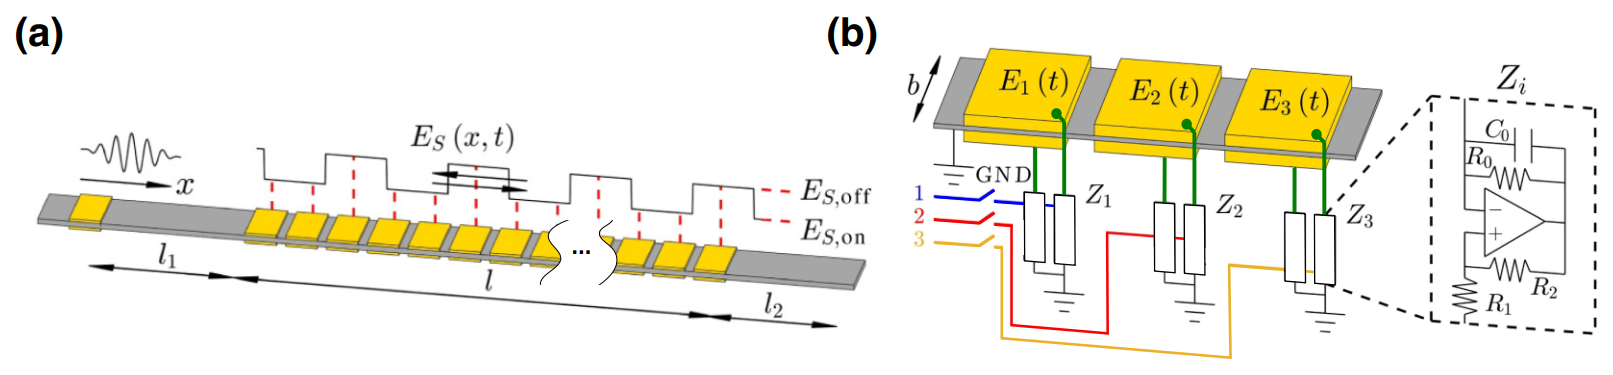
\includegraphics[width=0.9\textwidth]{img/experimental_setup_scheme.png}
        \caption{Beam substrate and array of piezoelectric patches (a), Spatio-Temporal cell and shunting circuits (b).}
    \end{figure}

    Out-of-plane velocity field is measured using a Polytec 3D laser Doppler vibrometer.

    \footnotetext[1]{For numerical values and detailed description, refer to the attached project report (Section 4.1).}

\end{frame}



\begin{frame}{Experimental setup}

    By connecting the piezoelectric patches to the beam, the effective properties of the system are modified.

    \vspace{9pt}

    \begin{columns}[c, onlytextwidth]

        \begin{column}{0.6\textwidth}

            \begin{figure}[H]

                \centering

                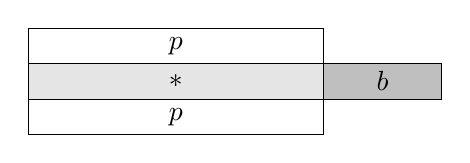
\begin{tikzpicture}[scale=1.5]

                    % Beam
                    \draw[fill=gray!20] (0,0) rectangle (2.5,0.3) node[midway] {$*$};
                    \draw[fill=gray!50] (2.5,0) rectangle (3.5,0.3) node[midway] {$b$};

                    % Piezoelectric patches
                    \draw[fill=white] (0, 0.3) rectangle (2.5, 0.6) node[midway] {$p$};
                    \draw[fill=white] (0, 0.0) rectangle (2.5, -0.3) node[midway] {$p$};

                \end{tikzpicture}

                \caption{Connection between piezoelectric patches and beam.}

            \end{figure}

        \end{column}

        \begin{column}{0.4\textwidth}

            \begin{equation}
                \begin{aligned}
                    EJ^*     & = E_b J_b + 2 E_p J_p       \\
                    \rho A^* & = \rho_b A_b + 2 \rho_p A_p
                \end{aligned}
            \end{equation}

        \end{column}

    \end{columns}

\end{frame}
\section{Theoretical background}
\label{sec:theoretical_background}

In order to understand the behavior of the system under investigation and the successive analysis performed on it, we need to introduce some theoretical concepts that are used throughout the report.

At first, a brief overview of the transversal wave equation in the case of beam element is given.
Then, the concept of piezoelectric patches is introduced, and the effect of their presence on the beam properties is studied.
Finally, the numerical methods used to solve the wave equation and analyze the system behavior are presented.

\subsection{Transversal wave equation for beam elements}
\label{subsec:transversal_wave_equation_beam_elements}

To recall the transversal wave equation for beam elements, we start by considering the equilibrium of forces acting on an infinitesimal element of the beam, as shown in Figure \ref{fig:beam_element_forces}.
We assume here small displacements and rotations, linear elastic material behavior (isotropic), homogeneous material properties, negligible damping, slender beam, and no tension or compression forces applied.

One can also recognize that these assumptions are similar to the ones made in the Euler-Bernoulli beam theory.
Thanks to the EB theory, we can also assume that the angular distortion produced in the beam by the action of shear forces is negligible and that the effect of rotational inertia is also negligible.
Based on these last assumptions, the following relation between the transversal displacement $w(x,t)$ and the bending moment $M(x,t)$ is obtained:

\begin{equation}
    M(x,t) = -EJ \frac{\partial^2 w(x,t)}{\partial x^2}
    \label{eq:bending_moment_transversal_displacement}
\end{equation}

Where $E$ is the Young's modulus, $J$ is the moment of inertia of the beam section, and $x$ is the coordinate along the beam axis.

\begin{figure}[H]
    \centering

    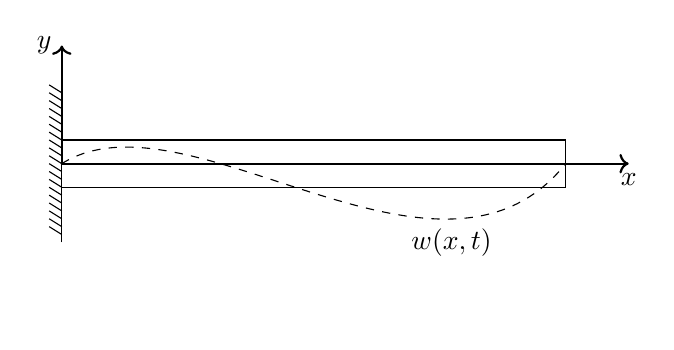
\begin{tikzpicture}[xscale=0.8]

        \draw (0, -0.3) rectangle (8, 0.3);

        \draw[->, thick] (0, 0) -- ++(9, 0) node[below]{$x$};
        \draw[->, thick] (0, 0) -- ++(0, 1.5) node[left]{$y$};
        \draw (0, -1) -- (0,  1);
        \draw[dashed] (0,0) .. controls (2, 1) and (6, -2) .. (8, 0) node[pos=0.75, below]{$w(x,t)$};

        \foreach \y in {-0.9, -0.8, ..., 0.9}
        \draw (0, \y) -- ++(-0.2, +0.1);

    \end{tikzpicture}
    \hspace{1cm}
    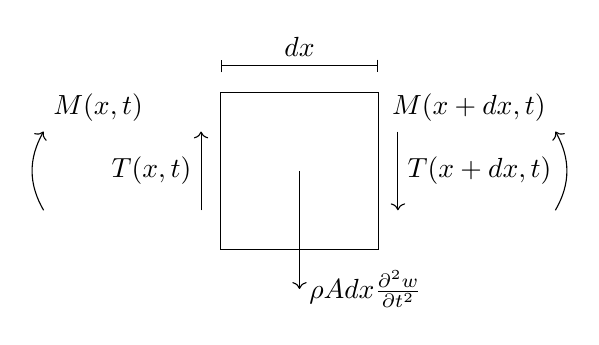
\begin{tikzpicture}

        \def\dx{2}
        \def\dy{2}

        \draw[|-|] (-\dx/2, +4/3*\dy/2) -- ++(\dx, 0) node[midway, above]{$dx$};

        \draw (-\dx/2, -\dy/2) rectangle (\dx/2, \dy/2);
        \draw[->] (0, 0) -- ++(0, -3/4*\dy) node[right]{$\rho A dx\frac{\partial^2 w}{\partial t^2}$};
        \draw[->] (-5/4*\dx/2, -\dy/4) -- ++(0, +1) node[midway, left]{$T(x, t)$};
        \draw[->] (+5/4*\dx/2, +\dy/4) -- ++(0, -1) node[midway, right]{$T(x + dx, t)$};
        \draw[->] (-13/4*\dx/2, -\dy/4) to [bend left] (-13/4*\dx/2, +\dy/4) node[above right]{$M(x, t)$};
        \draw[->] (+13/4*\dx/2, -\dy/4) to [bend right] (+13/4*\dx/2, +\dy/4) node[above left]{$M(x + dx, t)$};

    \end{tikzpicture}

    \caption{Transversal displacement $w(x,t)$ of a beam element and forces acting on infinitesimal element ($dx$).}
    \label{fig:beam_element_forces}

\end{figure}

Using D'Alambert principle, we can write the following vertical and rotational equilibrium for the infinitesimal element represented in Figure \ref{fig:beam_element_forces}:

\begin{equation}
    \begin{matrix}
        -M(x,t) + M(x + dx, t) - T(x,t) \frac{dx}{2} - T(x + dx, t) \frac{dx}{2} = 0 \\
        T(x, t) - T(x + dx, t) = \rho A dx \frac{\partial^2 w}{\partial t^2}
    \end{matrix}
\end{equation}

Using differential calculus, we can rewrite this equilibrium as:

\begin{equation}
    \begin{matrix}
        -M(x,t) + M(x, t) + \frac{\partial M(x,t)}{\partial x} dx - T(x,t) \frac{dx}{2} - T(x,t) \frac{dx}{2} - \frac{\partial T(x,t)}{\partial x} \frac{dx^2}{2} = 0 \\
        T(x, t) - T(x, t) - \frac{\partial T(x, t)}{\partial x} dx = \rho A dx \frac{\partial^2 w}{\partial t^2}
    \end{matrix}
\end{equation}

From which (neglecting higher order terms) we obtain:

\begin{equation}
    \begin{aligned}
        T(x, t)                            & = \frac{\partial M(x,t)}{\partial x}              \\
        \frac{\partial T(x,t)}{\partial x} & = - \rho A \frac{\partial^2 w(x,t)}{\partial t^2}
    \end{aligned}
\end{equation}

Substituting the expression of $T(x,t)$ and recalling the definition of $M(x, t)$ (see Equation \ref{eq:bending_moment_transversal_displacement}), we obtain the following equation of motion for the transversal displacement $w(x,t)$:

\begin{equation}
    \frac{\partial^2}{\partial x^2} \left( EJ \frac{\partial^2 w(x,t)}{\partial x^2} \right) = -\rho A \frac{\partial^2 w(x,t)}{\partial t^2}
    \label{eq:beam_equation_of_motion_transversal_displacement}
\end{equation}

It's easy to recognize that Equation \ref{eq:beam_equation_of_motion_transversal_displacement} is a fourth-order partial differential equation (PDE) in the space variable $x$ and a second-order PDE in the time variable $t$.

In case the material properties are constant both in time and space, $w(x,t)$ can be computed analytically as the product of a spatial function $\alpha(x)$ and a temporal function $\beta(t)$.
However, in the case of non-constant material properties, the problem becomes more complex and numerical methods are usually required to solve it.

\subsection{Piezoelectric patches analysis}
\label{subsec:piezoelectric_patches_analysis}

In this section, we introduce the necessary theory to address the use of piezoelectric patches in the system under investigation.

We start by recalling the general constitutive equations for piezoelectric materials before focusing on the specific case of piezoelectric patches bonded to a beam element.

\begin{figure}[H]
    \centering
    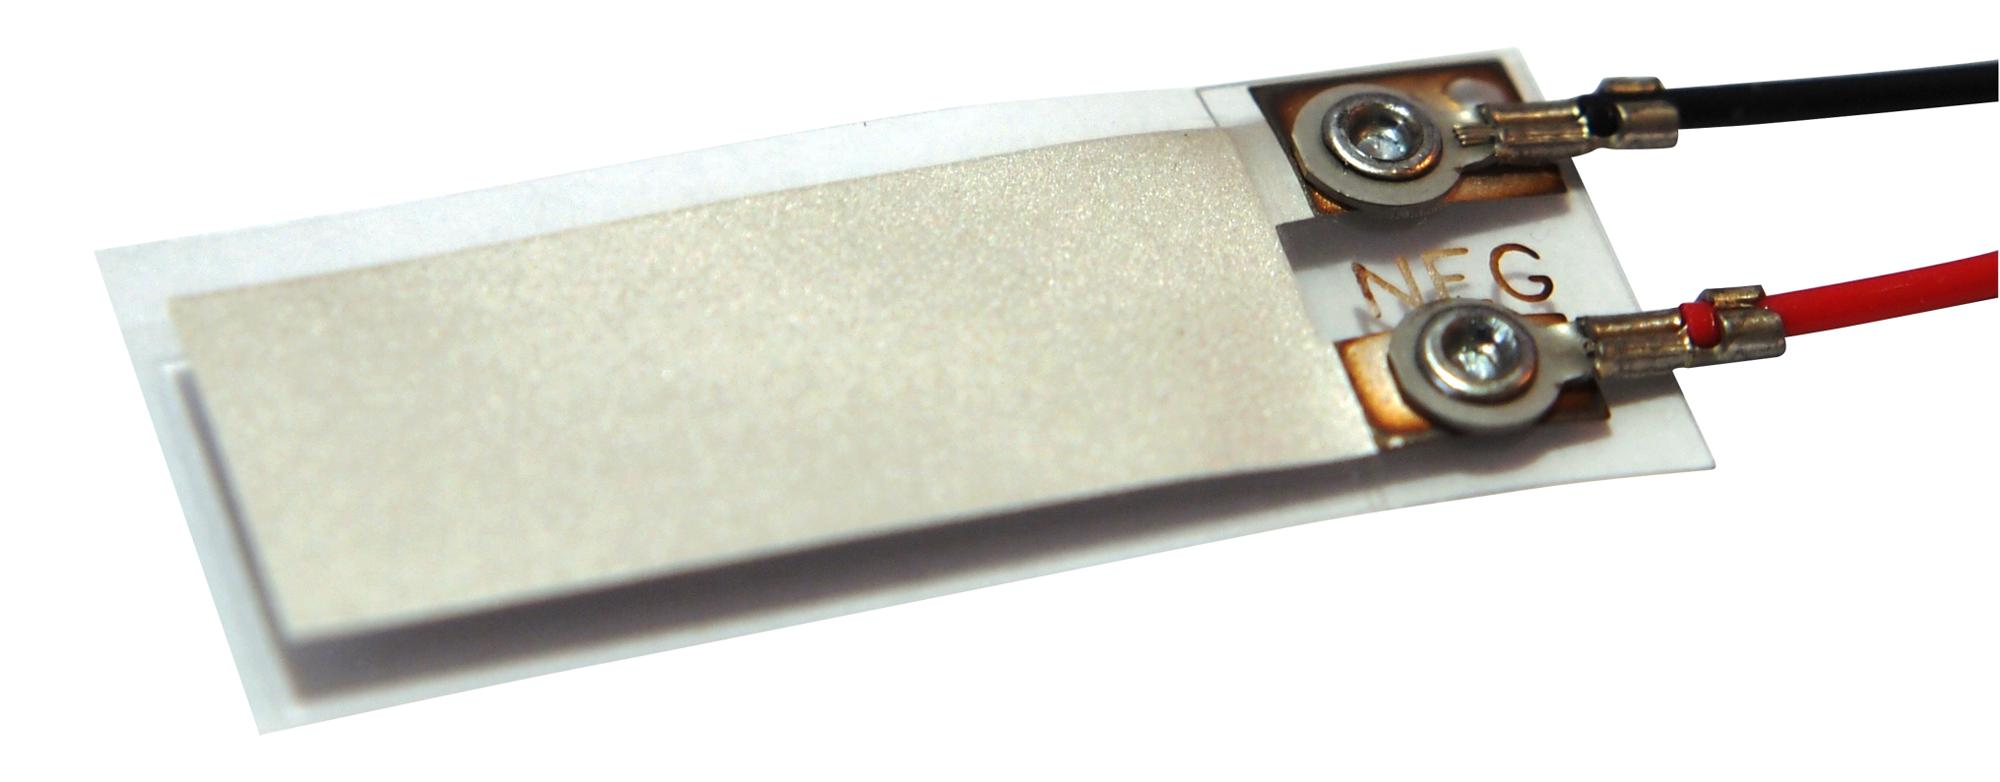
\includegraphics[width=0.5\textwidth]{img/piezo.jpg}
    \caption{Example of piezoelectric patch.}
    \label{fig:piezo}
\end{figure}


\subsubsection{Piezoelectric constitutive equations}
\label{subsubsec:piezoelectric_constitutive_equations}

Piezoelectric materials have the ability to convert mechanical energy into electrical energy and vice versa.
Considering to work within a reasonable range of deformations, the constitutive equations for piezoelectric materials can be linearized and written in matrix form as follows:

\begin{equation}
    \begin{bmatrix}
        \bm{D} \\
        \bm{S}
    \end{bmatrix} =
    \begin{bmatrix}
        \bm{\varepsilon}^T & \bm{d}   \\
        \bm{d}_t           & \bm{s}^E
    \end{bmatrix}
    \begin{bmatrix}
        \bm{E} \\
        \bm{T}
    \end{bmatrix}
\end{equation}

Where $\bm{S} [\Delta m / m]$ and $\bm{D} [C / m^2]$ are the mechanical strain and charge displacement vectors, $\bm{T} [N / m^2]$ and $\bm{E} [N / C]$ are the mechanical stress and electric field vectors, $\bm{s} [1 / Pa]$ is the compliance matrix, $\bm{d} [C / N]$ is the piezoelectric strain coefficient matrix, and $\bm{\varepsilon} [F / m]$ is the dielectric permittivity matrix.
Notice also that the superscript $()^T$ and $()^E$ indicate that the quantities are measured under constant stress and electric field, respectively, while the subscript $t$ indicates the transposition of the matrix.

Taking common assumptions as orthotropy of the material and neglecting any orthogonal piezoelectric effect, the constitutive equations can be greatly simplified forcing many of the coefficients to zero.

For the specific case of piezoelectric patches bonded to a beam element (as will be better shown in Section \ref{subsec:experimental_setup}), we can further simplify the constitutive equations by considering that the electric field is only acting in one direction, and study the stress and strain produced along one of the other normal directions.
In particular, referring to conventional piezoelectric theory, we are interested in the so-called $31$-mode, where the electric field is applied along the $3$-direction and the strain is measured in the $1$-direction (see Figure \ref{fig:piezo_31_operating_mode}).

\begin{figure}[H]
    \centering
    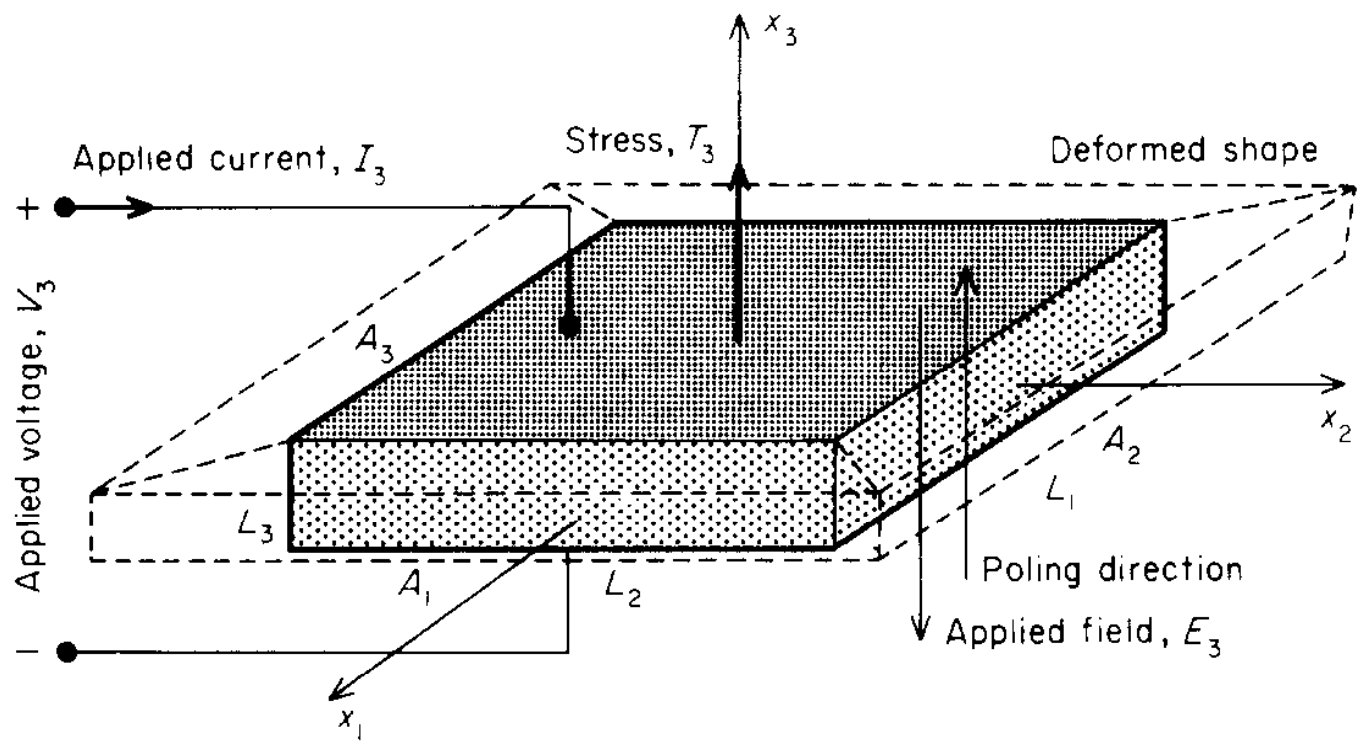
\includegraphics[width=0.7\textwidth]{img/piezo_31_operating_mode.png}
    \caption{Piezoelectric patch operating in $31$-mode.}
    \label{fig:piezo_31_operating_mode}
\end{figure}

Then, under the hypothesis that all the other quantities are zero, the constitutive equations can be written as:

\begin{equation}
    \begin{bmatrix}
        D_3 \\
        S_1
    \end{bmatrix} =
    \begin{bmatrix}
        \varepsilon_{33}^T & d_{31}   \\
        d_{13}             & s_{13}^E
    \end{bmatrix}
    \begin{bmatrix}
        E_3 \\
        T_1
    \end{bmatrix} =
    \begin{bmatrix}
        \varepsilon_{33}^T & d_{31}          \\
        d_{31}             & \frac{1}{Y_1^E}
    \end{bmatrix}
    \begin{bmatrix}
        E_3 \\
        T_1
    \end{bmatrix}
    \label{eq:piezoelectric_constitutive_equations}
\end{equation}

Notice that $\varepsilon_{33}^T$ is the dielectric permittivity in the $3$-direction when the stress in direction $1$ is zero ($T_1 = 0$), and $Y_1^E$ is the Young's modulus in the $1$-direction when the electric field in direction $3$ is zero ($E_3 = 0$).

Equation \ref{eq:piezoelectric_constitutive_equations} can also be rewritten in terms of applied voltage and current by performing the following change of variables and moving to Laplace domain:

\begin{equation}
    \begin{aligned}
        V & = \int_{0}^{L} E \cdot dx & \rightarrow &  & V(s) & = L \cdot E(s)  \\
        I & = \int_A D \cdot dA       & \rightarrow &  & I(s) & = sA \cdot D(s)
    \end{aligned}
\end{equation}

Substituting the expressions for $V$ and $I$ in the constitutive equations, we can obtain the following relationship:

\begin{equation}
    \begin{bmatrix}
        I_3 \\
        S_1
    \end{bmatrix} =
    \begin{bmatrix}
        sC_{3p}^T       & sA_3 d_{31}     \\
        d_{31} L_3^{-1} & \frac{1}{Y_1^E}
    \end{bmatrix}
    \begin{bmatrix}
        V_3 \\
        T_1
    \end{bmatrix}
    \label{eq:piezoelectric_constitutive_equations_volt_current}
\end{equation}

Where $C_p^T = A \varepsilon_{33}^T / L$ is the piezoelectric capacitance per unit length, and $L_3$ is the length of the piezoelectric patch in the $3$-direction.

An important final remark has to be made about the piezoelectric coupling coefficient $k_{31}$, which is defined as:

\begin{equation}
    k_{31} = \frac{d_{31} \sqrt{Y_1^E}}{\varepsilon_{33}^T} = \frac{d_{31}}{\sqrt{\varepsilon_{33}^T Y_1^E}}
\end{equation}

This coefficient is a measure of the efficiency of the piezoelectric material in converting mechanical energy into electrical energy and vice versa.
It's intuitive to understand that $0 < k_{31} < 1$, and the closer it is to $1$, the more efficient the material is in converting energy.


\subsubsection{Shunted piezoelectric patches}
\label{subsubsec:shunted_piezoelectric_patches}

The properties of a piezoelectric patch can be greatly influenced by the presence of a shunt circuit connected to it.
The successive analysis takes as reference the electrical scheme of Figure \ref{fig:shunted_piezoelectric_patch}.

\begin{figure}[H]
    \centering
    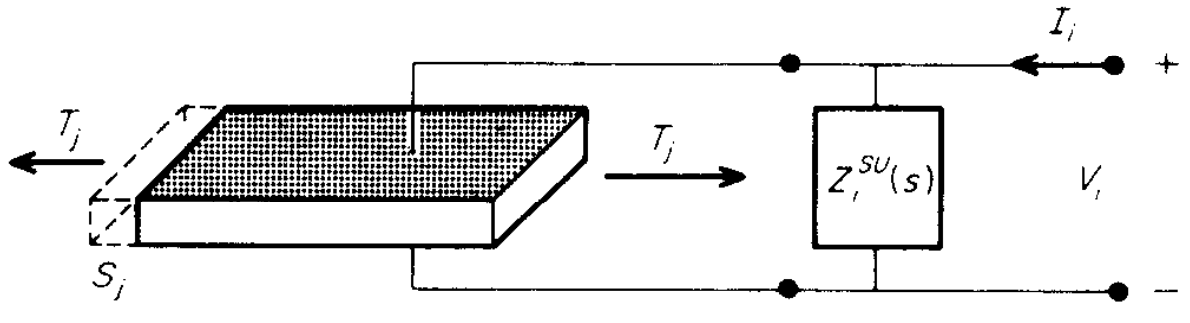
\includegraphics[width=0.7\textwidth]{img/piezo_shunted.png}
    \caption{Electrical scheme of a shunted piezoelectric patch.}
    \label{fig:shunted_piezoelectric_patch}
\end{figure}

In order to account for the presence of the shunt circuit, we need to adjust accordingly the electrical impedance of the system, given now as the parallel connection of the piezoelectric patch impedance $Z_p$ and the shunt impedance $Z_{su}$:

\begin{equation}
    Z^{EL} = \left( Z_p^{-1} + Z_{su}^{-1} \right)^{-1}
\end{equation}

% Or equivalently in terms of admittance:

% \begin{equation}
%     Y^{EL} = Z^{EL^{-1}} = Y_p + Y_{su} = sC_p^T + \frac{1}{Z_{su}}
% \end{equation}

Substituting the expression for $Y^{EL}$ in the constitutive equations (Equation \ref{eq:piezoelectric_constitutive_equations_volt_current}), we obtain the following relationship:

\begin{equation}
    \begin{bmatrix}
        I_3 \\
        S_1
    \end{bmatrix} =
    \begin{bmatrix}
        \frac{1}{Z^{EL}} & sA_3 d_{31}     \\
        d_{31} L_3^{-1}  & \frac{1}{Y_1^E}
    \end{bmatrix}
    \begin{bmatrix}
        V_3 \\
        T_1
    \end{bmatrix}
\end{equation}

Solving for the voltage across the piezoelectric patch, and then for the mechanical strain $S$, we can highlight the influence of the shunt circuit on the mechanical properties of the piezoelectric patch.

\begin{equation}
    \begin{aligned}
        V_3 & = Z^{EL} I_3 - Z^{EL} sA_3 d_{31} T_1                                                                                                                             \\
        S_1 & = d_{31} L_3^{-1} V_3 + \frac{1}{Y_1^E} T_1 = \left( d_{31} L_3^{-1} Z^{EL} \right) I_3 + \left( \frac{1}{Y_1^E} - d_{31} L_3^{-1} Z^{EL} sA_3 d_{31} \right) T_1
    \end{aligned}
\end{equation}

Recalling the traditional definition of stress and strain relationship $S = Y^E T$, we can recognize:

\begin{equation}
    \frac{1}{Y^{SU}} = \frac{1}{Y_1^E} - d_{31} L_3^{-1} Z^{EL} sA_3 d_{31}
\end{equation}

Where $Y^{SU}$ is the mechanical admittance of the piezoelectric patch.
It's clear that the presence of the shunt have a direct influence on the mechanical properties of the piezoelectric patch, and thus on the beam element to which it might be bonded.

In the optic of this work, it's of particular interest to obtain a clear equation of the type $Y^{SU} = f(Y_p, Z_{su})$ that can be used to study the influence of the shunt impedance on the mechanical properties of the piezoelectric patch.
In particular, rearranging the terms of the last equation, we can obtain the following expression:

\begin{equation}
    Y^{SU} = Y_1^D \left( 1 - \frac{k_{31}^2}{1 + s C_p^S Z^{SU}} \right)
    \label{eq:mechanical_admittance_shunted_piezoelectric_patch}
\end{equation}


\subsection{Numerical methods for wave propagation analysis}
\label{subsec:numerical_methods_for_wave_propagation_analysis}

In this section, we introduce the numerical methods used to simulate the wave propagation in a generic modulated beam structure.
In particular, one of the main results that can be obtained by using these methods is the dispersion relation of the system, which describes the relationship between the frequency and the wavenumber of the propagating waves.
Once the dispersion relation is known, it is possible to analyze the behavior of the system under different conditions and to design the structure to achieve specific properties as will be shown in the following sections.

The following methods are introduced:

\begin{itemize}
    \item Transfer Matrix Method (TMM): used to analyze the wave propagation in case of purely spatial modulation structure;
    \item Plane Wave Expansion Method (PWEM): allow considering not only space modulation but also time modulation;
    \item Finite Difference Time Domain (FDTD) method: a general-purpose method that can be used to simulate a large family of problems requiring the solution of partial differential equations.
\end{itemize}



\subsubsection{Transfer Matrix Method (TMM)}
\label{subsubsec:transfer_matrix_method_tmm}

One of the most common methods used to analyze the wave propagation in a beam structure is the Transfer Matrix Method (TMM).

The main idea of the TMM is to consider and analyze the system as a series of interconnected elements, each one characterized by a transfer matrix that relates the states at the left and right of the element.
By setting continuity between the states at the boundaries of the elements, and imposing the periodicity of the solution via Floquet theorem, it is possible to obtain the dispersion relation of the system solving an eigenvalue problem.

Given that with the TMM it's not possible to account for time-varying material properties, we limit our analysis to the case of beam structures with spatially varying material properties only, modelled by the following equation of motion:

\begin{equation}
    \frac{\partial^2}{\partial x^2} \left( E J(x) \frac{\partial^2 w(x,t)}{\partial x^2} \right) = - \rho A(x) \frac{\partial^2 w(x,t)}{\partial t^2}
\end{equation}

Based on the equation above, we can define the state vector $y(x)$ as the displacement $w(x,t)$ and its derivatives up to $w^{(3)}(x,t)$.
We can also give a physical interpretation to the state vector considering instead the displacement, slope, bending moment, and shear force of the beam:

\begin{equation}
    y(x) =
    \begin{bmatrix}
        v(x)      \\
        \theta(x) \\
        M(x)      \\
        T(x)
    \end{bmatrix} =
    \begin{bmatrix}
        w(x)                                     \\
        \frac{\partial w(x)}{\partial x}         \\
        -EJ \frac{\partial^2 w(x)}{\partial x^2} \\
        -EJ \frac{\partial^3 w(x)}{\partial x^3}
    \end{bmatrix}
\end{equation}

Once the state vector is defined, we write the governing equation of motion in the state-space form:

\begin{equation}
    \frac{\partial y(x)}{\partial x} = A(x) y(x) =
    \begin{bmatrix}
        0                  & 1 & 0                & 0 \\
        0                  & 0 & \frac{-1}{EJ(x)} & 0 \\
        0                  & 0 & 0                & 1 \\
        \omega^2 \rho A(x) & 0 & 0                & 0
    \end{bmatrix} y(x)
\end{equation}

Where $\omega$ is the angular frequency of the travelling wave in the beam.
The solution of the equation above can be written as:

\begin{equation}
    y(x) = T(x) y(0) = e^{x A(x)} y(0)
\end{equation}

Imposing now the continuity of the states at the boundaries of the elements, we can write the transfer matrix of the system as:

\begin{equation}
    T = T(x_r) T(x_{r-1}) \ldots T(x_1) = \prod_{i=r}^{1} T(x_i)
\end{equation}

Which leads to the following periodicity condition in space:

\begin{equation}
    y(x + \lambda_m) = T y(x)
\end{equation}

Notice, however, that the Floquet theorem can also be used to impose periodicity in space, and combined with the above equation, it leads to the following eigenvalue problem:

\begin{equation}
    \begin{aligned}
        y(x + \lambda_m) & = T y(x)         \\
        y(x + \lambda_m) & = e^{i \mu} y(x)
    \end{aligned}
    \rightarrow
    T y(x) = e^{i \mu} y(x)
    \label{eq:transfer_matrix_method_eigenvalue_problem}
\end{equation}

Where $\mu$ is the Floquet exponent or the non-dimensional wavenumber, and it can be used to obtain the dispersion relation of the system given that $\mu = \kappa \lambda_m$.

It's clear how the TMM corresponds to an inverse solution for the dispersion, given that the eigenvalue problem in Equation \ref{eq:transfer_matrix_method_eigenvalue_problem} can be solved to obtain the Floquet exponent $\mu$ as a function of the angular frequency $\omega$, on which $T$ depends.



\subsubsection{Plane Wave Expansion Method (PWEM)}
\label{subsubsec:plane_wave_expansion_method_pwem}

The Plane Wave Expansion Method (PWEM) is a numerical method used to solve plane waves in periodic structures.
Its more general version, often referred to as Generalized Plane Wave Expansion Method (GPWEM), allows for the analysis of waves without any restriction on the form of the wave itself.
The main advantage with respect to the TMM is that the PWEM can be used to analyze not only spatially varying material properties but also time-varying ones.

The idea here is to move to the frequency domain via Fourier series expansion and, upon the imposition of the periodicity of the solution via Floquet theorem, to solve the wave equation which will now be in the form of a Quadratic Eigenvalues Problem (QEP).
A main difference with respect to the TMM is that the solution of the PWEM is a direct one, meaning that the dispersion relation is obtained by imposing the wavenumber $\kappa$ and solving for the frequency $\omega$.

For the problem at hand, we consider dealing with structural beam properties varying both in space and in time, with a periodicity dictated by $\lambda_m$ and $T_m$ respectively.
The Fourier series expansion of the structural properties then reads:

\begin{equation}
    \begin{aligned}
        \begin{aligned}
            EJ(x, t) & = \sum_{m,n} \left[ \frac{1}{\lambda_m T_m} \int_{-\frac{\lambda_m}{2}}^{\frac{\lambda_m}{2}} \int_{-\frac{T_m}{2}}^{\frac{T_m}{2}} EJ(x, t) e^{-i (m\kappa_m x - n\omega_m t)}dx dt \right] e^{i (m\kappa_m x - n\omega_m t)} \\
                     & = \sum_{m,n} \widehat{EJ}_{m,n} e^{i (m\kappa_m x - n\omega_m t)}
        \end{aligned} \\
        \begin{aligned}
            \rho A(x, t) & = \sum_{m,n} \left[ \frac{1}{\lambda_m T_m} \int_{-\frac{\lambda_m}{2}}^{\frac{\lambda_m}{2}} \int_{-\frac{T_m}{2}}^{\frac{T_m}{2}} \rho A(x, t) e^{-i (m\kappa_m x - n\omega_m t)}dx dt \right] e^{i (m\kappa_m x - n\omega_m t)} \\
                         & = \sum_{m,n} \widehat{\rho A}_{m,n} e^{i (m\kappa_m x - n\omega_m t)}
        \end{aligned}
    \end{aligned}
\end{equation}

With similar fashion, we can impose the Floquet solution to the displacement $w(x, t)$ and expand it in the frequency domain as:

\begin{equation}
    w(x, t) = e^{i (\kappa x - \omega t)} \sum_{p, q} \widehat{w}_{p,q} e^{i (p\kappa_m x - q\omega_m t)}
\end{equation}

After some nontrivial algebraic manipulations, that include the integration over the space and time domains and the application of the orthogonality of the Fourier series, the wave equation can be rewritten in the following form:

\begin{equation}
    \sum_{p, q} \left( p \kappa_m + \kappa \right)^2 \left( s \kappa_m + \kappa \right)^2 \widehat{EJ}_{s-p, r-q} \widehat{w}_{p,q} = \sum_{p, q} \left( q \omega_m + \omega \right) \left( r \omega_m + \omega \right) \widehat{\rho A}_{s-p, r-q} \widehat{w}_{p,q}
    \label{eq:plane_wave_expansion_method_wave_equation}
\end{equation}

Equation \ref{eq:plane_wave_expansion_method_wave_equation} is basically the equivalent of Equation \ref{eq:beam_equation_of_motion_transversal_displacement} in the frequency domain, considering $P$ and $Q$ as the number of harmonics in space and time respectively.

The solution of Equation \ref{eq:plane_wave_expansion_method_wave_equation} can be obtained by solving the Quadratic Eigenvalues Problem (QEP) associated to Equation \ref{eq:plane_wave_expansion_method_wave_equation} for the frequency $\omega$ as a function of the wavenumber $\kappa$.
In particular, the QEP can be written as:

\begin{equation}
    \left( \omega^2 L_2 (\kappa) + \omega L_1 (\kappa) + L_0 (\kappa) \right) \widehat{w} = 0
\end{equation}

Where $L_2 (\kappa)$ and $L_1 (\kappa)$ are in some sense associated to the mass matrices of the system, while $L_0 (\kappa)$ represent the equivalent stiffness matrix given as a summation of contributions relative to both the flexural stiffness ($EJ$) and the inertial properties ($\rho A$) of the beam.
Notice also that the size of the QEP is $(2Q + 1)\times(2P + 1)$, which can be bottleneck in terms of computational resources given that it should be solved for each value of the wavenumber $\kappa$.



\subsubsection{Finite Difference Time Domain (FDTD) method}
\label{subsubsec:finite_difference_time_domain_fdtd_method}

The Finite Difference Time Domain (FDTD) method is a general-purpose method used to solve partial differential equations.
It operates by discretizing both the spatial and temporal domains and approximating differential operators using finite differences.

By adopting a Taylor series expansion, the second-order and fourth-order finite difference approximations for a function $f(x)$ are given by:

\begin{equation}
    \frac{\partial^2 f(x)}{\partial x^2} \approx \frac{f(x + \Delta x) - 2 f(x) + f(x - \Delta x)}{\Delta x^2}
    \label{eq:finite_difference_second_order}
\end{equation}

\begin{equation}
    \frac{\partial^4 f(x)}{\partial x^4} \approx \frac{f(x + 2 \Delta x) - 4 f(x + \Delta x) + 6 f(x) - 4 f(x - \Delta x) + f(x - 2 \Delta x)}{\Delta x^4}
    \label{eq:finite_difference_fourth_order}
\end{equation}

As done in the Section \ref{subsubsec:plane_wave_expansion_method_pwem}, we can consider a beam structure with properties varying both in space and in time (periodicity dictated by $\lambda_m$ and $T_m$ respectively).

One could directly apply the finite difference method to Equation \ref{eq:beam_equation_of_motion_transversal_displacement}, but this would require to compute the displacement in a given cell based on the derivative of the displacement of the neighboring cells.
Instead, in order to avoid relying on possibly cumulative approximations, we introduce a dummy variable $v(x,t)$ such that its second spatial derivative corresponds to the displacement $w(x,t)$.
The problem can now be rewritten as:

\begin{equation}
    \begin{cases}
        EJ(x, t) \frac{\partial^4 v(x,t)}{\partial x^4} = - \rho A(x, t) \frac{\partial^2 v(x,t)}{\partial t^2} \\
        w(x,t) = \frac{\partial^2 v(x,t)}{\partial x^2}
    \end{cases}
\end{equation}

Discretizing the space and time domains and applying finite difference approximations (Equations \ref{eq:finite_difference_second_order} in time and \ref{eq:finite_difference_fourth_order} in space), we derive the following set of update equations:

\begin{equation}
    \begin{cases}
        \begin{aligned}
            v(t + \Delta t, x) = &
            -\left( \frac{c(x, t)^2 \Delta t}{\Delta x^2} \right)^2
            \left[ v(t, x + 2\Delta x) - 4 v(t, x + \Delta x) + 6 v(t, x) - 4 v(t, x - \Delta x) + v(t, x - 2\Delta x) \right] + \\
                                 & + 2 v(t, x) - v(t - \Delta t, x)                                                              \\
        \end{aligned} \\
        w(t + \Delta t, x) = \frac{1}{\Delta x^2} \left[ v(t + \Delta t, x + \Delta x) - 2 v(t + \Delta t, x) + v(t + \Delta t, x - \Delta x) \right]
    \end{cases}
\end{equation}

Where $c(x, t) = (EJ(x, t) / \rho A(x, t))^{1/4}$ is the equivalent traversal wave speed in the beam.


\paragraph{Boundary conditions}

Boundary conditions can be enforced by setting appropriate values for the displacement and dummy variable at the domain limits.
Dirichlet boundary conditions, for instance, can be implemented by setting the displacement to zero at the boundaries ($w(t, x_{min}) = w(t, x_{max}) = 0$).

On the other hand, given that we are dealing with finite domains, it's also important to avoid or at least minimize the reflection of the waves at the boundaries.
To do so, one can simply introduce a buffer zone along the space dimension with properties equal to the ones of the beam structure so that the waves can travel through it without being reflected back in the domain of interest.
Simulation time can also be tuned in order to minimize the reflection of the waves back from the boundaries.

Excitation forces can be imposed at selected points by modifying the values of the displacement and the dummy variable at the corresponding locations at each time step of the simulation.


\paragraph{Stability condition}

The numerical stability of the FDTD method is governed by the Courant-Friedrichs-Lewy (CFL) condition, which dictates the maximum allowable time step to ensure stable wave propagation.
The idea is that the simulated wave should not travel faster than the speed of the wave in the real system.

The CFL condition is given by:

\begin{equation}
    \left( \frac{max|c(x, t)^2| \Delta t}{\Delta x^2} \right)^2 \leq C_{max}
\end{equation}

Where $C_{max}$ is a constant that depends on the specific problem under investigation, but it that can be set to $1$ in most cases.


\section{Analysis of the shunted piezoelectric patches}
\label{sec:analysis_shunted_piezo}

In Section \ref{subsec:piezoelectric_patches_analysis} we have introduced the concept of shunted piezoelectric patches and we have shown how the mechanical admittance of the piezoelectric patch is influenced by the electrical impedance of the shunt circuit.

In this section, we want to further characterize this relationship by analyzing the effects of different shunt circuits on the system.
A sensitivity analysis is performed by considering the connection of the piezoelectric patches to a host beam structure and by analyzing the position of the band-gaps in the dispersion relation of the system.
While different shunting layouts are presented in the paragraph below, for the sensitivity analysis we focus on the RLC circuit only, as it is the one that is also used in the experimental analysis.

Successively, for the case of shunt circuits composed by active elements, we proposed a breif stability analysis.


\paragraph{Shunt circuits layouts}

As for the shunt circuits, three different layouts can be considered, as shown in Figure \ref{fig:shunt_layouts}.

\begin{figure}[H]

    \begin{minipage}{0.27\textwidth}

        \centering

        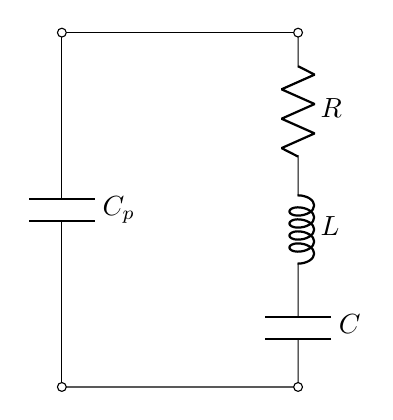
\begin{tikzpicture}[european voltages]

            % Upper and lower horizontal lines
            \draw (0,0) to [short] ++(3,0);
            \draw (0,-4.5) to [short] ++(3,0);

            % Piezo
            \draw (0,0) to [C, l=$C_p$, o-o] ++(0,-4.5);

            % Shunt
            \draw (3,0)
            to [R, l=$R$, o-] ++(0,-2)
            to [L, l=$L$] ++(0,-1)
            to [C, l=$C$, -o] ++(0,-1.5);

        \end{tikzpicture}

    \end{minipage}
    %
    \hfill
    %
    \begin{minipage}{0.31\textwidth}

        \centering

        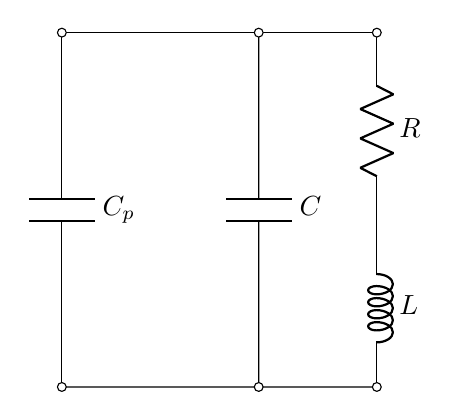
\begin{tikzpicture}[european voltages]

            % Upper and lower horizontal lines
            \draw (0,0) to [short] ++(4,0);
            \draw (0,-4.5) to [short] ++(4,0);

            % Piezo
            \draw (0,0) to [C, l=$C_p$, o-o] ++(0,-4.5);

            % Shunt capacitor
            \draw (2.5,0) to [C, l=$C$, o-o] ++(0,-4.5);

            % Shunt resistor and inductor
            \draw (4,0) to [R, l=$R$, o-] ++(0,-2.5) to [L, l=$L$, -o] ++(0,-2);

        \end{tikzpicture}

    \end{minipage}
    %
    \hfill
    %
    \begin{minipage}{0.31\textwidth}

        \centering

        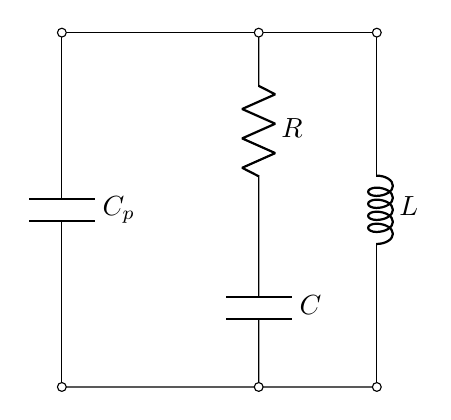
\begin{tikzpicture}[european voltages]

            % Upper and lower horizontal lines
            \draw (0,0) to [short] ++(4,0);
            \draw (0,-4.5) to [short] ++(4,0);

            % Piezo
            \draw (0,0) to [C, l=$C_p$, o-o] ++(0,-4.5);

            % Shunt capacitor
            \draw (2.5,0) to [R, l=$R$, o-] ++(0,-2.5) to [C, l=$C$, -o] ++(0,-2);

            % Shunt resistor and inductor
            \draw (4,0) to [L, l=$L$, o-o] ++(0,-4.5);

        \end{tikzpicture}

    \end{minipage}

    \caption{Shunt layouts: (a) Series $RLC$ shunt, (b) Parallel $RL//C$ shunt, (c) Parallel $RC//L$ shunt.}
    \label{fig:shunt_layouts}

\end{figure}

From basic circuit theory, we can write the electrical impedance of the three shunt circuits as follows:

\begin{equation}
    \begin{aligned}
        Z_{su}^{RLC}   & = R + sL + \frac{1}{sC}                                                                                          \\
        Z_{su}^{RL//C} & = \left(\frac{1}{R + sL} + sC\right)^{-1} = \frac{R + sL}{1 + (R + sL)sC} = \frac{R + sL}{1 - \omega^2LC - sRC}  \\
        Z_{su}^{RC//L} & = \left(\frac{1}{R + \frac{1}{sC}} + \frac{1}{sL} \right)^{-1} = \frac{-\omega^2 RLC + sL}{1 - \omega^2LC - sRC}
    \end{aligned}
    \label{eq:shunt_circuits_impedance}
\end{equation}

Where $s = j\omega$ is the complex frequency and $\omega$ is the angular frequency.



\paragraph{Negative capacitance realization}

When thinking to classical electrical components it's obvious, from an energetic point of view, that the values of $R$, $L$, and $C$ must be all non-negative.
However, thanks to the use of appropriate external circuits, it is possible to realize equivalent electrical components having negative values.
In particular, given that this is also the case in the experimental approach, we consider the possibility of having negative capacitance in the shunt circuits.

In order to realize a negative capacitance, the circuit depicted in Figure \ref{fig:negative_capacitance_realization} can be used.

\begin{figure}[H]
    \centering
    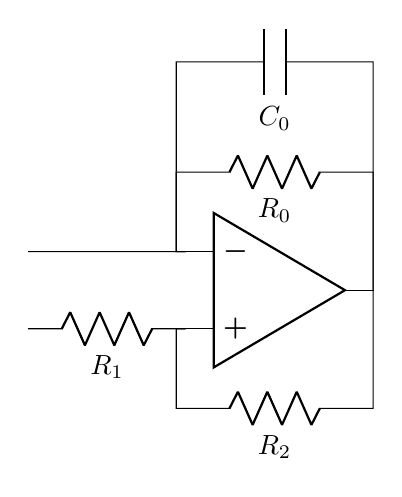
\begin{tikzpicture}[european voltages]

        \node[op amp] (OPAMP) {};

        \draw(OPAMP.out) to [short] ++(0, +2.9) to [C, l=$C_0$] ++(-2.5, 0) |- (OPAMP.-);
        \draw(OPAMP.out) to [short] ++(0, +1.5) to [R, l=$R_0$] ++(-2.5, 0) |- (OPAMP.-);
        \draw(OPAMP.out) to [short] ++(0, -1.5) to [R, l=$R_2$] ++(-2.5, 0) |- (OPAMP.+);

        \draw(OPAMP.-) to [short] ++(-2, 0);
        \draw(OPAMP.+) to [R, l=$R_1$] ++(-2, 0);

    \end{tikzpicture}
    \caption{Negative capacitance realization using an OP-AMP.}
    \label{fig:negative_capacitance_realization}

\end{figure}

The circuit depicted in Figure \ref{fig:negative_capacitance_realization} is equivalent to a negative capacitance having the following value:

\begin{equation}
    C_{eq} = -C_N = -\frac{R_1}{R_2} \left(\frac{1}{R_0} + sC_0\right)^{-1}
    \label{eq:negative_capacitance_real}
\end{equation}

One can notice the presence of the resistance $R_0$ parallel to the capacitance $C_0$.
While $R_1$ and $R_2$ are used to scale the value of the negative capacitance, $R_0$ is a key component of the circuit that enable a bias path for the current flowing through the negative capacitance avoiding the saturation of the OP-AMP.
Ideally, $R_0$ should be infinite, leading to the following expression for the ideal negative capacitance:

\begin{equation}
    C_{eq} = -C_N = -\frac{R_1}{R_2} \left(sC_0\right)^{-1}
    \label{eq:negative_capacitance_ideal}
\end{equation}

Of course, being the OP-AMP an active element powered by an external power supply, its presence in the circuit can lead to instability issues.
A dedicated analysis focusing on this aspect is proposed in Section \ref{subsec:stability_analysis}.


\subsection{Sensitivity analysis}
\label{subsec:sensitivity_analysis}

For the study of the system's band-gaps, we consider the connection of the piezoelectric patches to a beam structure as shown in Figure \ref{fig:beam_piezo_patches}.
The same numerical values for the geometry and material properties used in the experimental setup are considered (see Section \ref{subsec:experimental_setup}).

\begin{figure}[H]

    \centering

    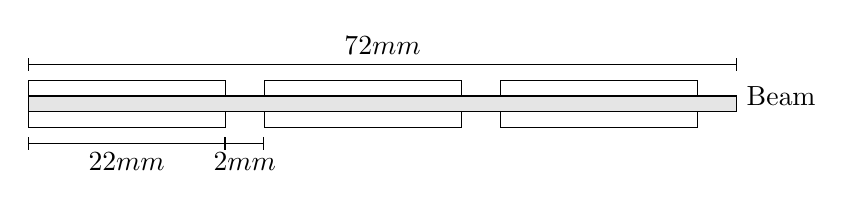
\begin{tikzpicture}

        % Beam
        \draw[fill=gray!20] (0,0) rectangle (9,0.2) node[right] {Beam};

        \draw[|-|] (0,0.6) -- (9,0.6) node[pos=.5, above] {$72 mm$};
        \draw[|-|] (0,-0.4) -- (2.5,-0.4) node[pos=.5, below] {$22 mm$};
        \draw[|-|] (2.5,-0.4) -- (3,-0.4) node[pos=.5, below] {$2 mm$};


        \foreach  \i in {0,1,2}
            {
                % Piezo patches
                \draw[fill=white] (3*\i, 0.2) rectangle (2.5 + 3*\i, 0.4);
                \draw[fill=white] (3*\i, 0.0) rectangle (2.5 + 3*\i, -0.2);
            }

    \end{tikzpicture}

    \caption{Unit cell composed by a beam substrate and 3 pairs of piezoelectric patches.}
    \label{fig:beam_piezo_patches}

\end{figure}

Intuitively, the presence of the piezoelectric patches will cause a change in the mechanical properties of the beam.
For simplicity, a weighted average of the mechanical properties of the beam and the piezoelectric patches is considered:

\begin{equation}
    \begin{aligned}
        J^*    & = J_b + 2 J_p                                   \\
        A^*    & = A_b + 2 A_p                                   \\
        E^*    & = \frac{E_b J_b + 2 E_p J_p}{J_b + 2 J_p}       \\
        \rho^* & = \frac{\rho_b A_b + 2 \rho_p A_p}{A_b + 2 A_p}
    \end{aligned}
    \label{eq:weighted_average_mechanical_properties}
\end{equation}


\subsubsection{$RLC_N$ shunt circuit}
\label{subsubsec:RLC_shunt_circuit_negative_capacitance}

The electrical impedance of an $RLC_N$ shunt circuit is given by Equation \ref{eq:shunt_circuits_impedance}, in which $C$ takes the form of $-C_N$.
By substitution in Equation \ref{eq:mechanical_admittance_shunted_piezoelectric_patch}, we obtain the mechanical admittance of the piezoelectric patch connected to the $RLC_N$ shunt circuit as:

\begin{equation}
    Y^{SU} = Y_1^D \left( 1 - \frac{k_{31}^2}{1 + s C_p^S \left( R + sL - \frac{1}{sC_N} \right)} \right) = Y_1^D \left( 1 - \frac{k_{31}^2}{1 + C_p^S \left( -\frac{1}{C_N} - \omega^2 L \right) - s C_p^S R} \right)
    \label{eq:mechanical_admittance_RLC_shunt}
\end{equation}

It's intuitive to think that the presence of the shunt circuit will cause a variation in the piezoelectric coupling coefficient.
This means that via a proper choice of the shunt circuit parameters, it's possible to control the mechanical admittance of the piezoelectric patch and, consequently, the band-gap of the system.
In particular, the new coupling coefficient can be written as:

\begin{equation}
    (k_{31}^{SU})^2 = \frac{k_{31}^2}{1 + C_p^S \left( -\frac{1}{C_N} - \omega^2 L \right) - s C_p^S R}
    \label{eq:coupling_coefficient_RLC_shunt}
\end{equation}

By analyzing the above equation, it's possible to understand that $R$ act as damping factor being multiplied by the complex frequency $s$.
This means that $R$ can be used to control the width and the depth of the band-gap.
On the other hand, $L$ and $C_N$ can be used to shift the band-gap to lower or higher frequencies, given that their contribution decreases or increases the stiffness of the undergoing structure.

The following figures, shows the dispersion relation of the system for different values of $R$, $L$, and $C$.
All the plots are obtained by using the Transfer Matrix Method (TMM).


\paragraph{Short circuit case}

In the short circuit case, the impedance of the shunt circuit is given by $Z_{su} = 0 \Omega$.
In this case, the mechanical admittance of the piezoelectric patch is actually the same as the one of the piezoelectric patch itself $Y^{SU} = Y_1^E$ in the null electric field case.

\begin{figure}[H]
    \centering
    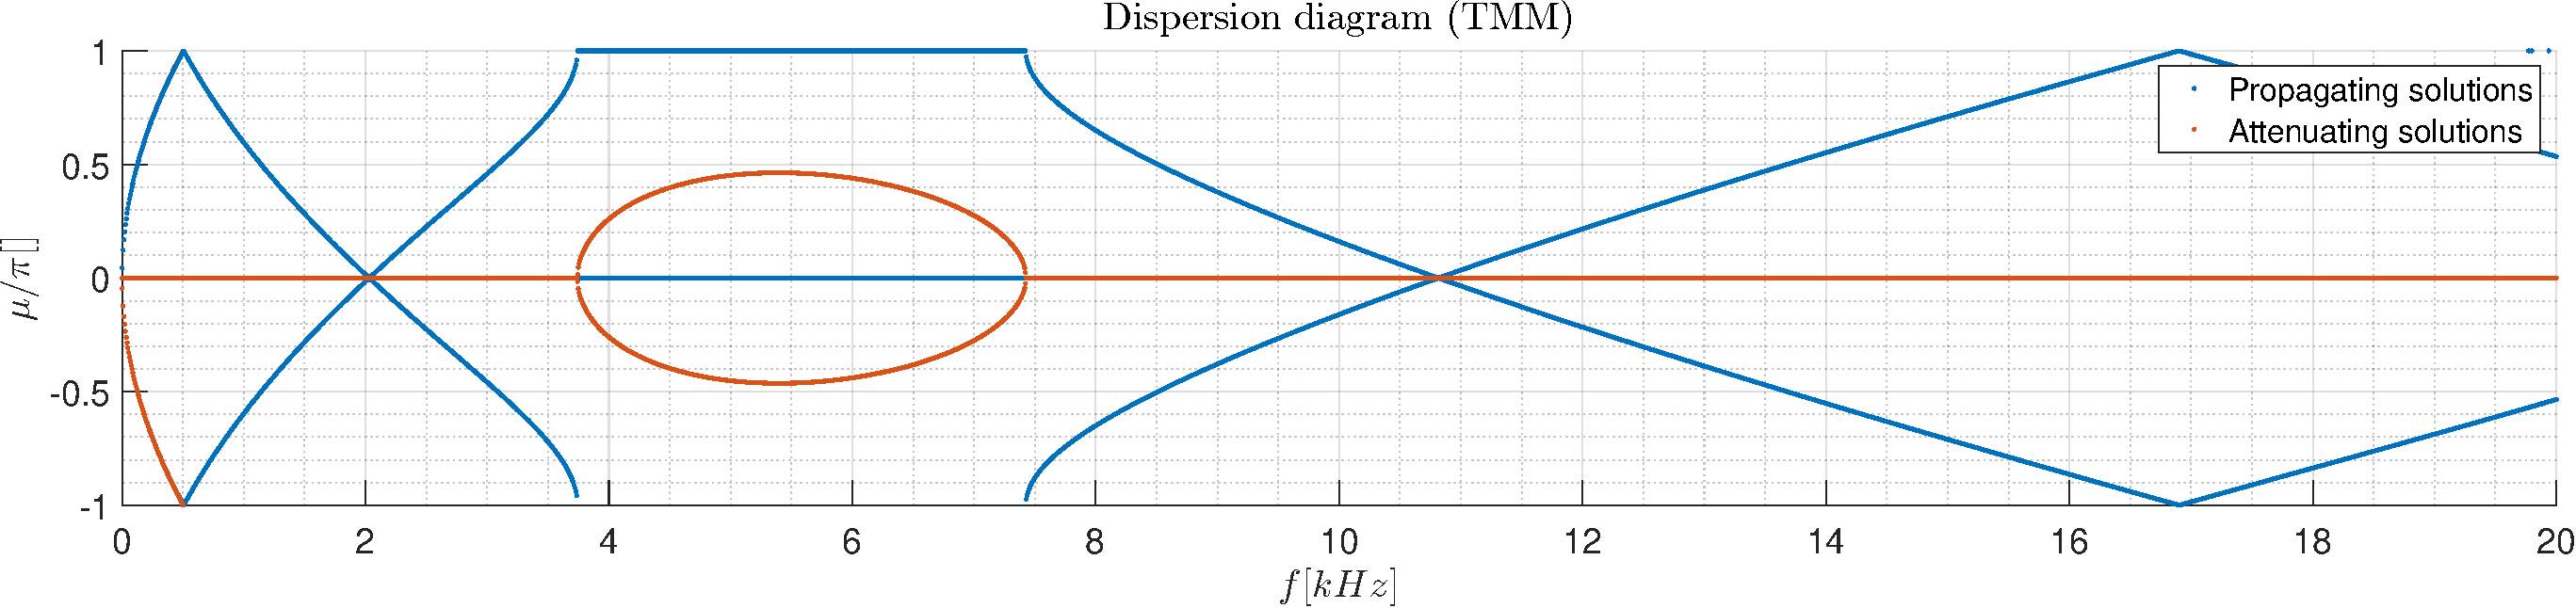
\includegraphics[width=\textwidth]{./img/MATLAB/TMM_ON-ON-ON_OFF_R1000_L0.015_C5e-09.pdf}
    \caption{Short circuit case.}
    \label{fig:TMM_ON-ON-ON_OFF_R1000_L0.015_C5e-09.pdf}
\end{figure}


\paragraph{Open circuit case}

In the open circuit case, the impedance of the shunt circuit is given by $Z_{su} = \infty \Omega$.
In this case, for the mechanical admittance of the piezoelectric patch, we have $Y^{SU} = Y_1^D$.
The dispersion relation of the system is shown in Figure \ref{fig:TMM_ON-ON-ON_+inf_R1000_L0.015_C5e-09.pdf}.

\begin{figure}[H]
    \centering
    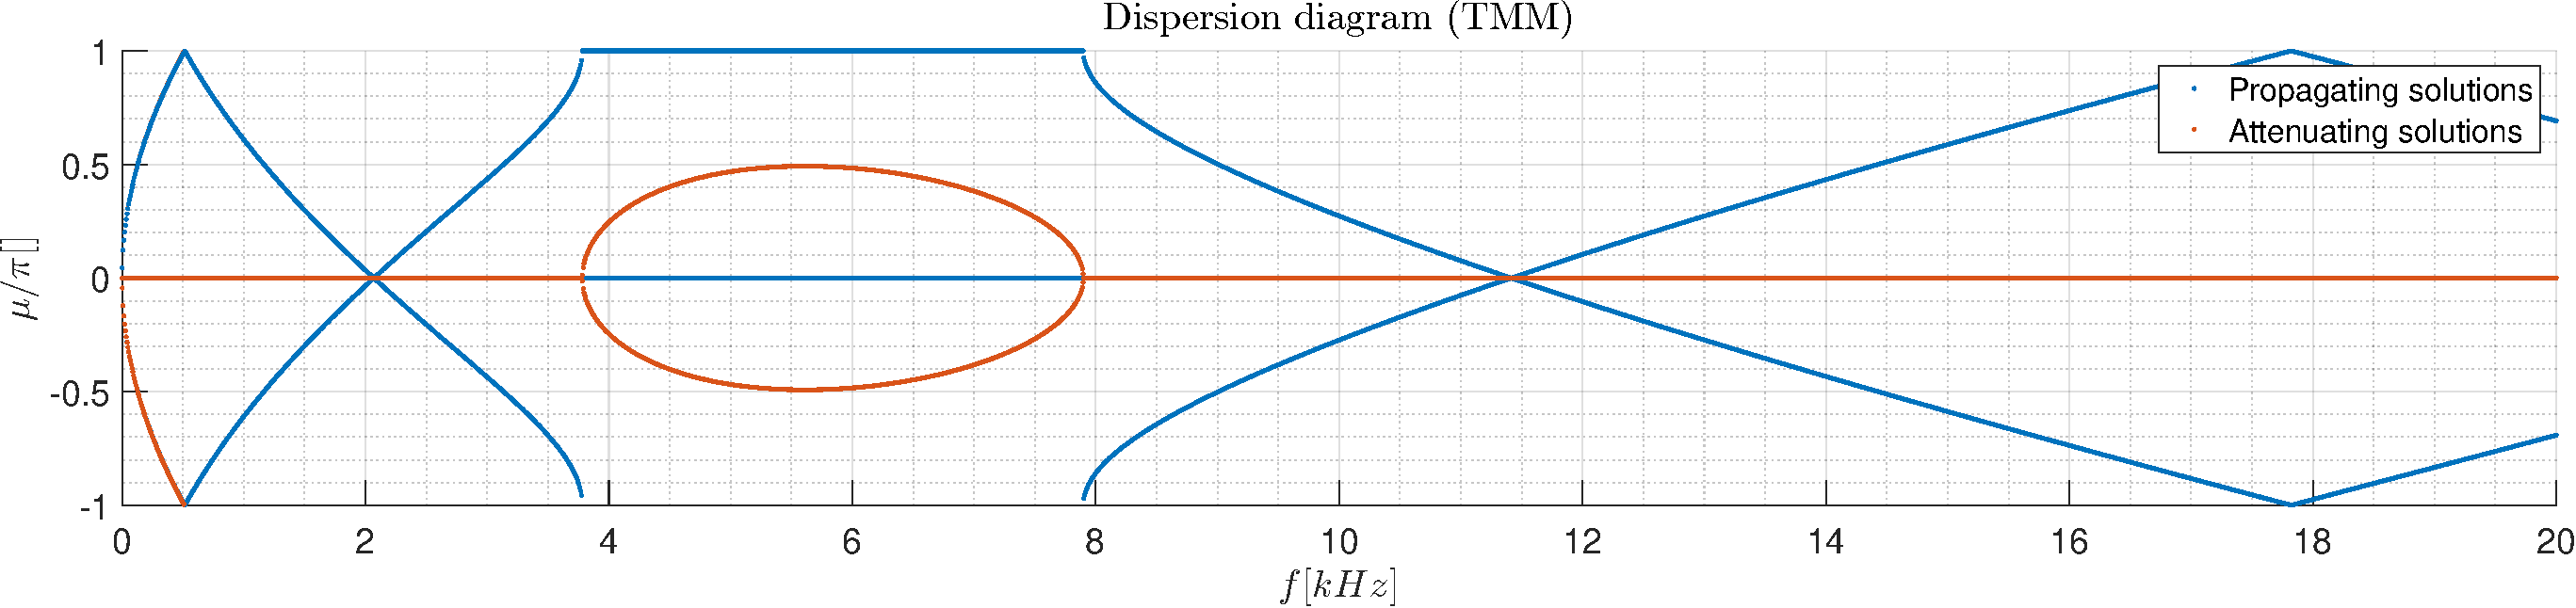
\includegraphics[width=\textwidth]{./img/MATLAB/TMM_ON-ON-ON_+inf_R1000_L0.015_C5e-09.pdf}
    \caption{Open circuit case.}
    \label{fig:TMM_ON-ON-ON_+inf_R1000_L0.015_C5e-09.pdf}
\end{figure}

With respect to the short circuit case, the band-gap is shifted to higher frequencies due to the fact that the structure is now stiffer ($Y_1^D > Y_1^E$).


\paragraph{$L$ shunt circuit}

In the case of a purely inductive shunt circuit, the impedance is given by $Z_{su} = sL$, and the equation for the mechanical admittance of the piezoelectric patch reduces to:

\begin{equation}
    Y^{SU} = Y_1^D \left( 1 - \frac{k_{31}^2}{1 -\omega^2 C_p^S L} \right)
    \label{eq:mechanical_admittance_R_shunt}
\end{equation}

For the analysis, four values of $L$ are considered while $R$ and $C_N$ are kept constant at $0 \Omega$ and $\infty F$, respectively.

\begin{table}[H]
    \centering
    \begin{tabular}{|c|c|c|}
        \hline
        $R$ [$\Omega$] & $L$ [H] & $C_N$ [F] \\
        \hline
        0              & 0.00    & $\infty$  \\
        0              & 0.02    & $\infty$  \\
        0              & 0.10    & $\infty$  \\
        0              & 1.00    & $\infty$  \\
        \hline
    \end{tabular}
    \caption{Values of $R$, $L$, and $C_N$ for the purely inductive shunt circuit.}
    \label{tab:RLC_N_values_L_case}
\end{table}

One can also visualize the effect of the inductive element on the system by plotting $Y^{SU}$ for the different values of $L$.

\begin{figure}[H]
    \centering
    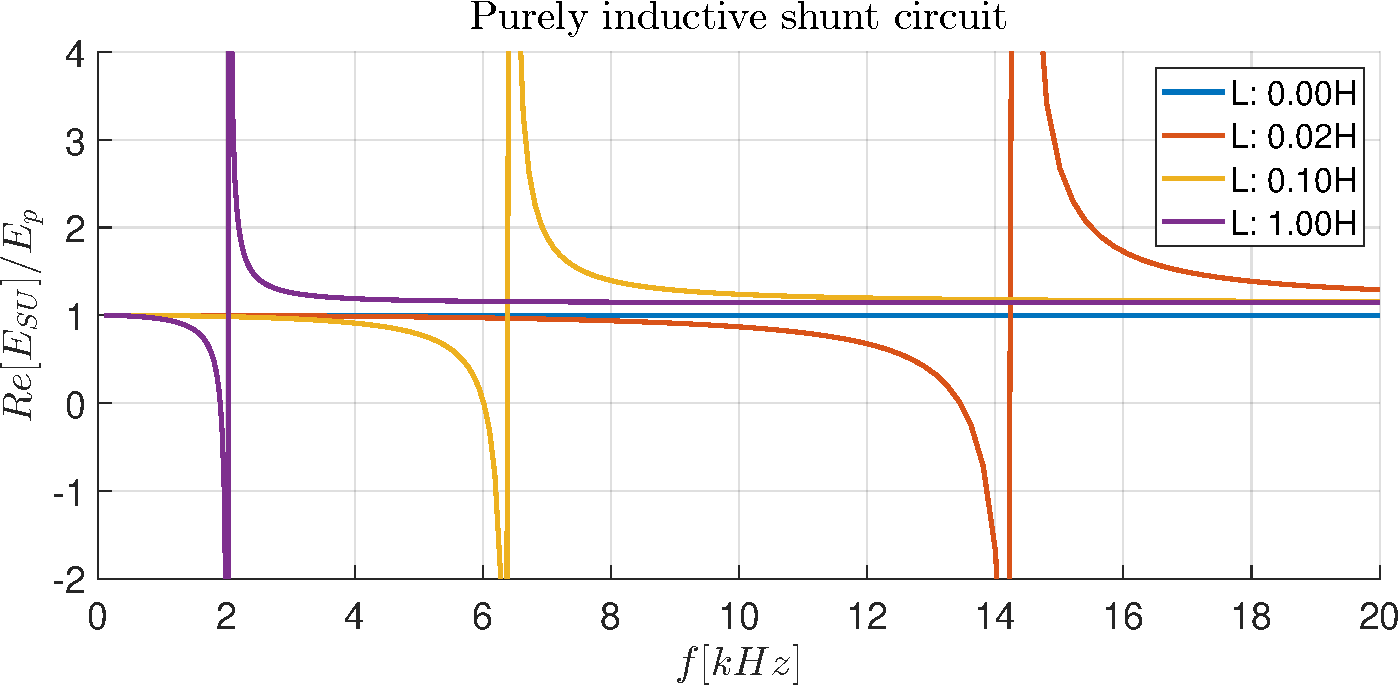
\includegraphics[width=0.6\textwidth]{./img/MATLAB/Y_SU_Purely inductive shunt circuit.pdf}
    \caption{Analysis of $Y^{SU}$ for the purely inductive shunt circuit.}
    \label{fig:Y_SU_Purely_inductive_shunt_circuit.pdf}
\end{figure}

Instead, the dispersion relation of the system are shown in the figures below.

\begin{figure}[H]
    \centering
    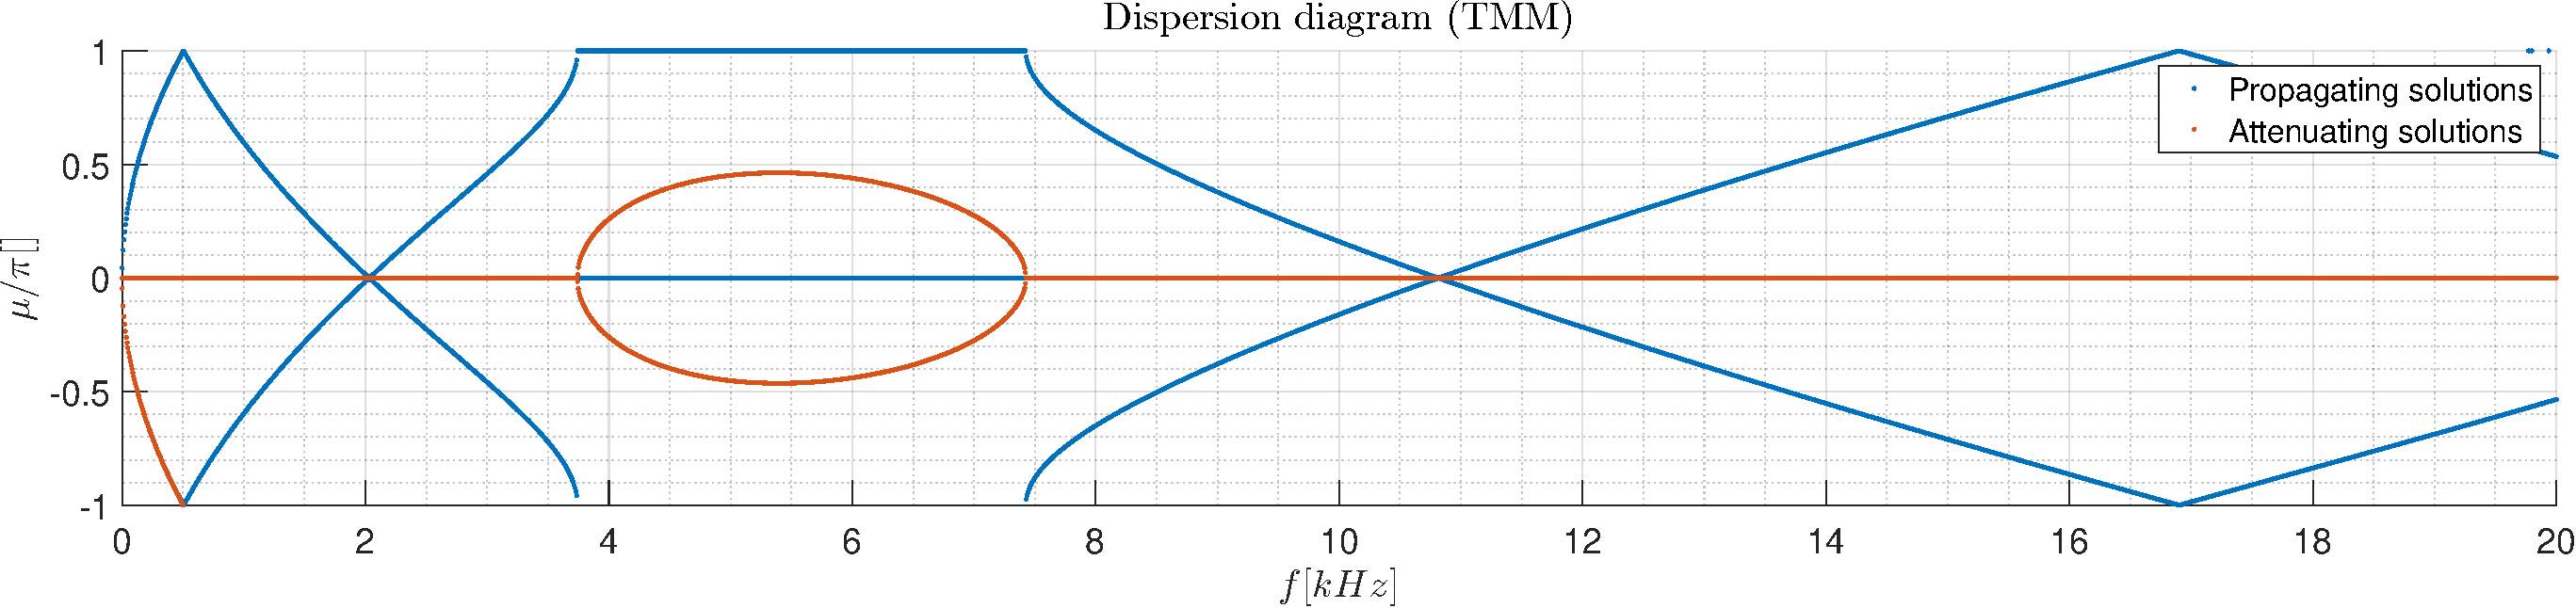
\includegraphics[width=\textwidth]{./img/MATLAB/TMM_ON-ON-ON_RLC_R0_L0_CInf.pdf}
    \caption{RLC shunt circuit with $R = 0 \Omega$, $L = 0 H$, and $C = \infty F$.}
    \label{fig:TMM_ON-ON-ON_RLC_R0_L0_CInf.pdf}
\end{figure}

\begin{figure}[H]
    \centering
    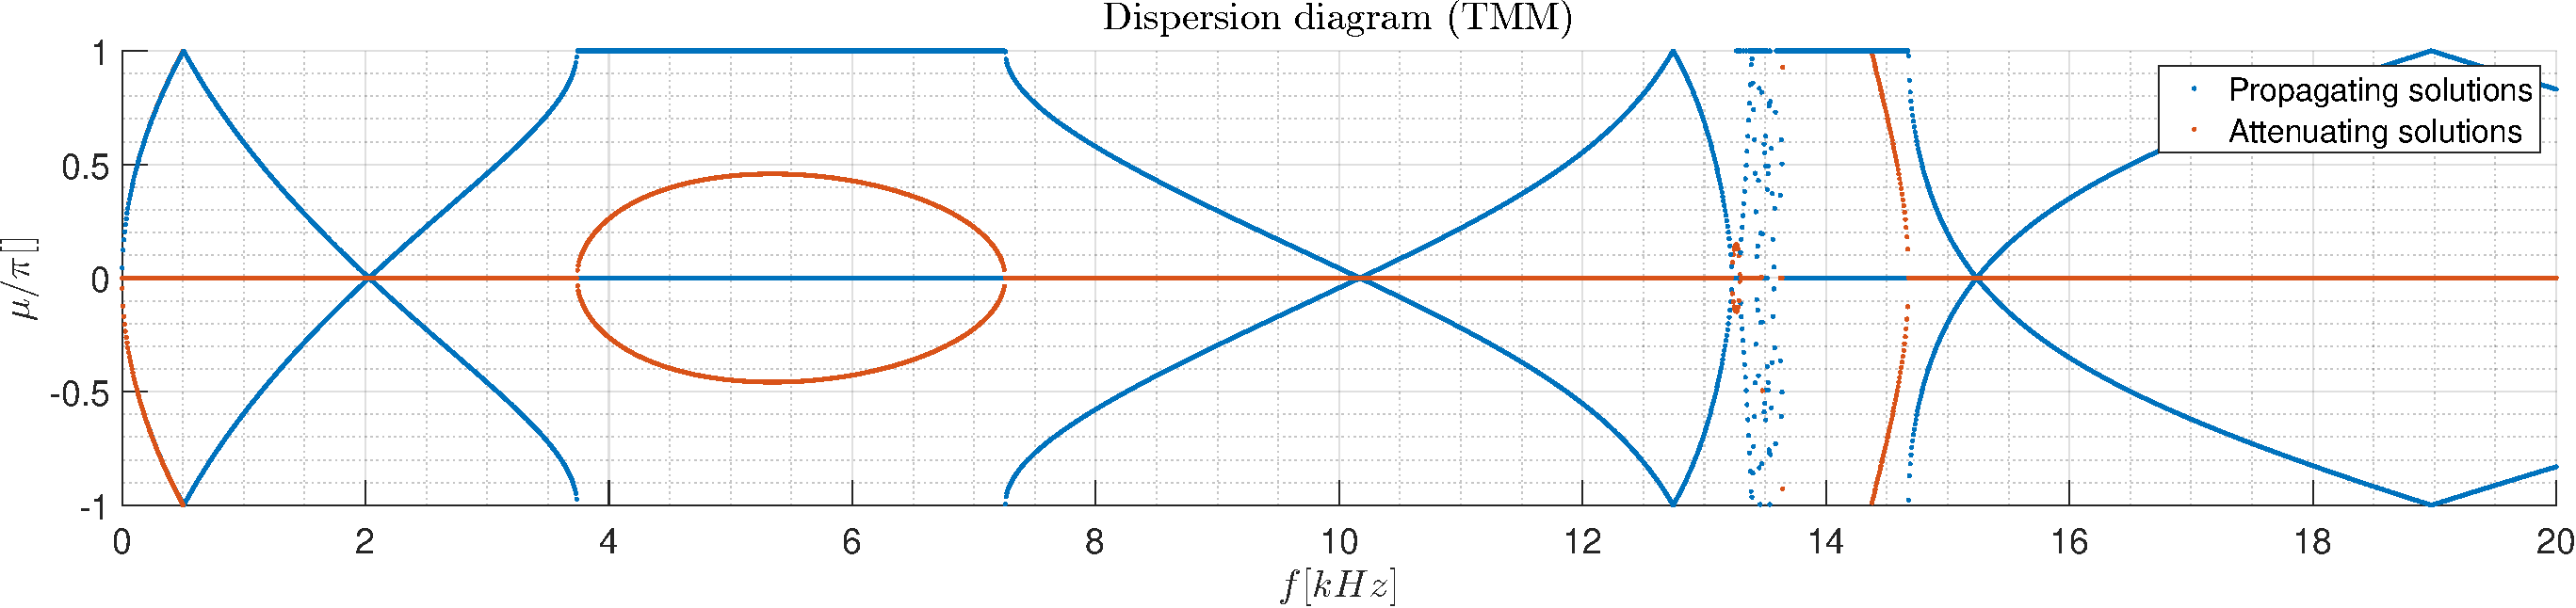
\includegraphics[width=\textwidth]{./img/MATLAB/TMM_ON-ON-ON_RLC_R0_L0.02_CInf.pdf}
    \caption{RLC shunt circuit with $R = 0 \Omega$, $L = 0.02 H$, and $C = \infty F$.}
    \label{fig:TMM_ON-ON-ON_RLC_R0_L0.02_CInf.pdf}
\end{figure}

\begin{figure}[H]
    \centering
    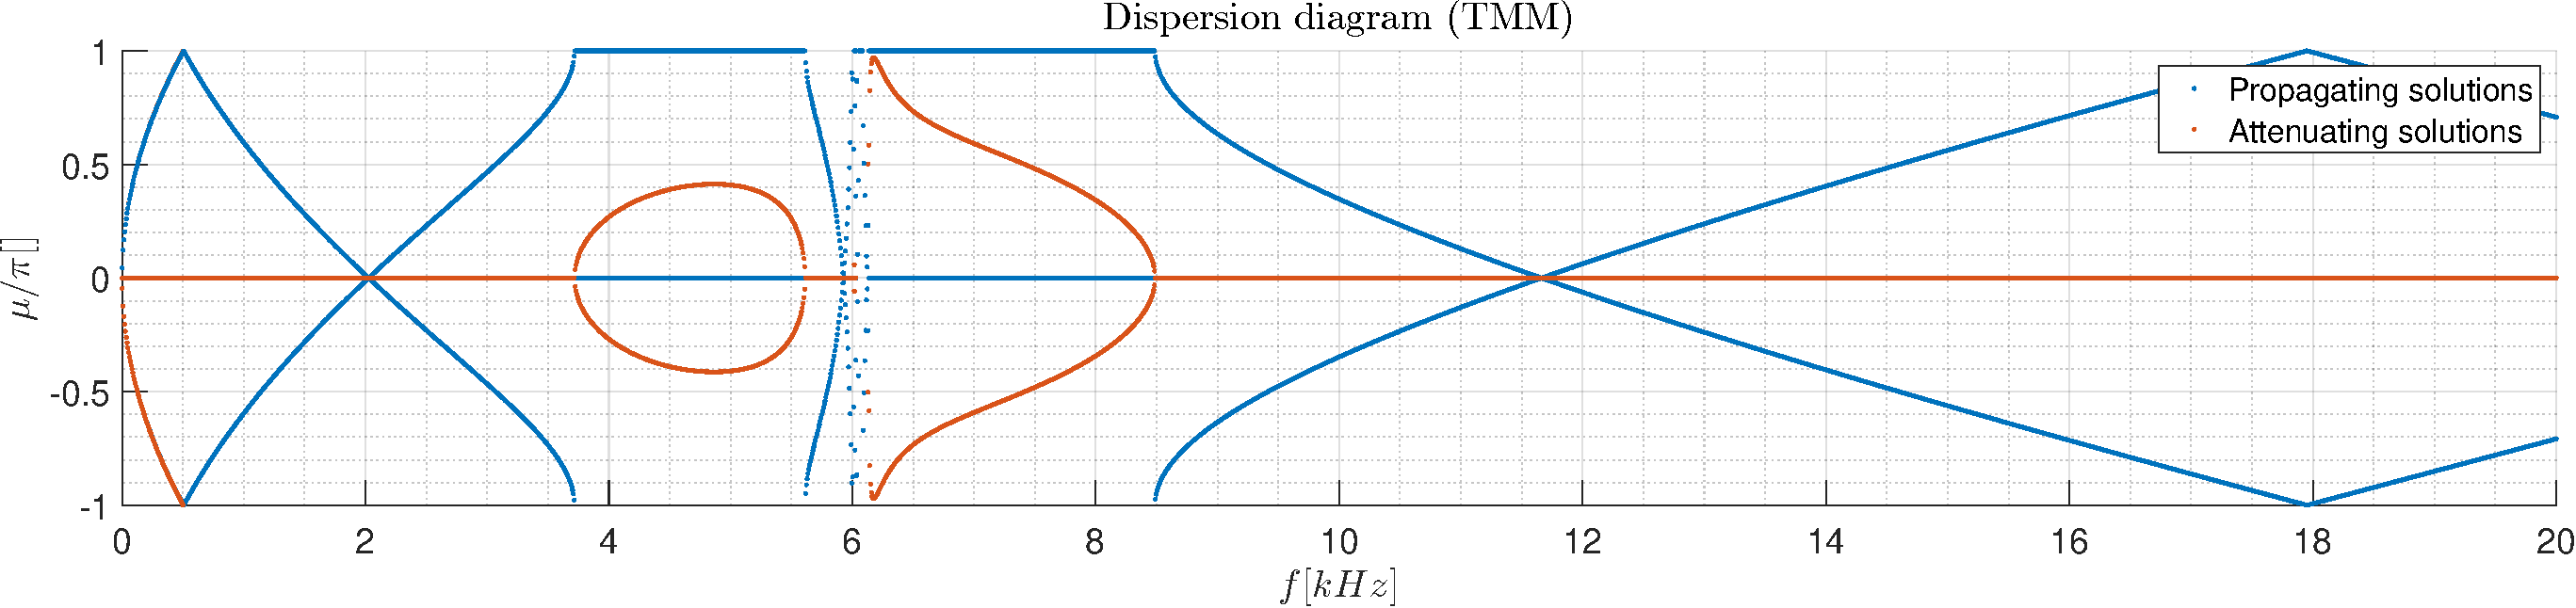
\includegraphics[width=\textwidth]{./img/MATLAB/TMM_ON-ON-ON_RLC_R0_L0.1_CInf.pdf}
    \caption{RLC shunt circuit with $R = 0 \Omega$, $L = 0.10 H$, and $C = \infty F$.}
    \label{fig:TMM_ON-ON-ON_RLC_R0_L0.1_CInf.pdf}
\end{figure}

\begin{figure}[H]
    \centering
    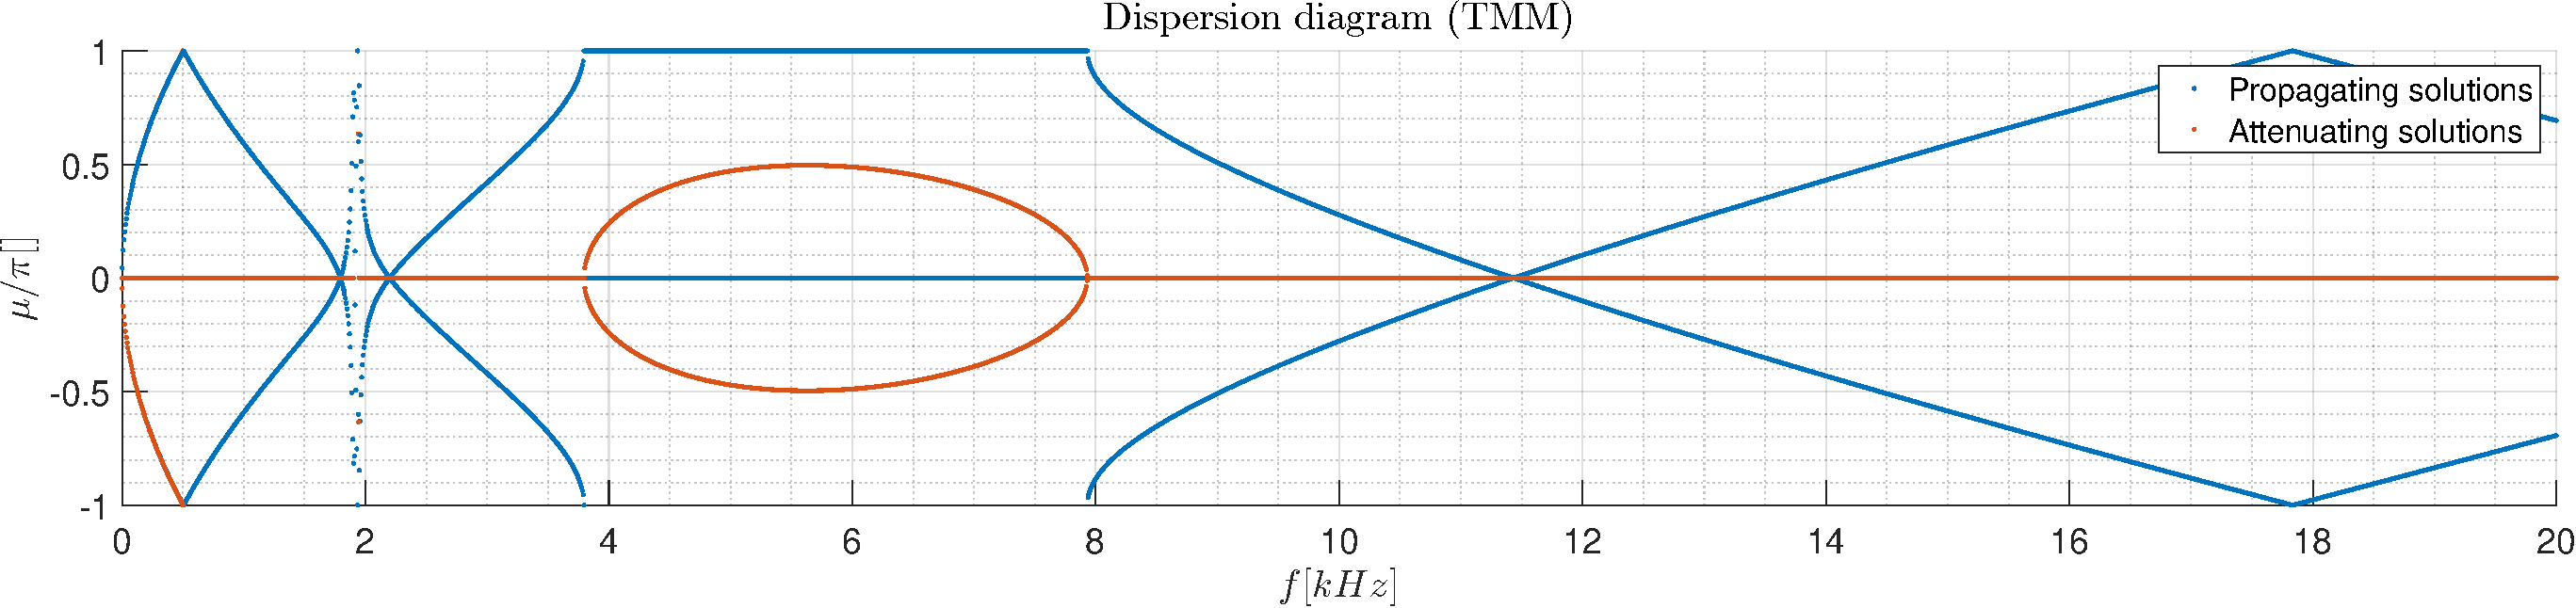
\includegraphics[width=\textwidth]{./img/MATLAB/TMM_ON-ON-ON_RLC_R0_L1_CInf.pdf}
    \caption{RLC shunt circuit with $R = 0 \Omega$, $L = 1 H$, and $C = \infty F$.}
    \label{fig:TMM_ON-ON-ON_RLC_R0_L1_CInf.pdf}
\end{figure}

Based also on Figure \ref{fig:Y_SU_Purely_inductive_shunt_circuit.pdf}, it's possible to observe that at low frequencies the system behaves as in the short circuit case, while at higher frequencies the system behaves as in the open circuit case.
Moreover, the lower $L$, the higher the frequency at which the transition between the two behaviors occurs.
The transition frequency between the two behaviors is given by:

\begin{equation}
    1 - \omega^2 C_p^S L = 0 \rightarrow \omega_n = \frac{1}{\sqrt{C_p^S L}}
\end{equation}

When the natural frequency falls within the band-gap, a splitting of the band-gap occurs, as shown in Figure \ref{fig:TMM_ON-ON-ON_RLC_R0_L0.1_CInf.pdf}.
One might use this effect to create an isolated band-pass filter.


\paragraph{$RL$ shunt circuit}

In the case of a resistive-inductive shunt circuit, the impedance is given by $Z_{su} = R + sL$.
The equation for the mechanical admittance of the piezoelectric patch is:

\begin{equation}
    Y^{SU} = Y_1^D \left( 1 - \frac{k_{31}^2}{1 -\omega^2 C_p^S L - s C_p^S R} \right)
    \label{eq:mechanical_admittance_RL_shunt}
\end{equation}

For the analysis, four values of $R$ are considered while $L$ and $C_N$ are kept constant at $0.03 H$ and $\infty F$, respectively.

\begin{table}[H]
    \centering
    \begin{tabular}{|c|c|c|}
        \hline
        $R$ [$\Omega$] & $L$ [H] & $C_N$ [F] \\
        \hline
        0              & 0.03    & $\infty$  \\
        50             & 0.03    & $\infty$  \\
        200            & 0.03    & $\infty$  \\
        1000           & 0.03    & $\infty$  \\
        \hline
    \end{tabular}
    \caption{Values of $R$, $L$, and $C_N$ for the resistive-inductive shunt circuit.}
    \label{tab:RLC_N_values_RL_case}
\end{table}

One can also visualize the effect of the resistive element on the system by plotting $Y^{SU}$ for the different values of $R$.

\begin{figure}[H]
    \centering
    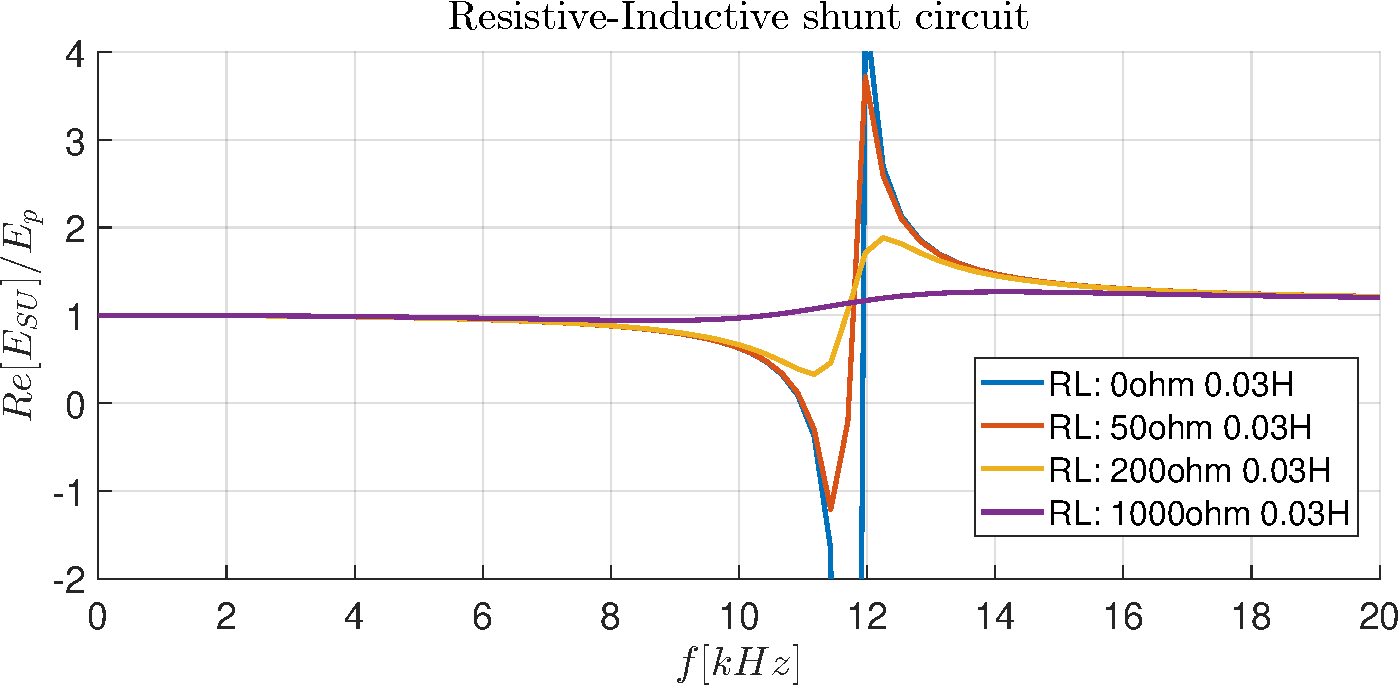
\includegraphics[width=0.6\textwidth]{./img/MATLAB/Y_SU_Resistive-Inductive shunt circuit.pdf}
    \caption{Analysis of $Y^{SU}$ for the resistive-inductive shunt circuit.}
    \label{fig:Y_SU_Resistive-Inductive_shunt_circuit.pdf}
\end{figure}

Instead, the dispersion relation of the system are shown in the figures below.

\begin{figure}[H]
    \centering
    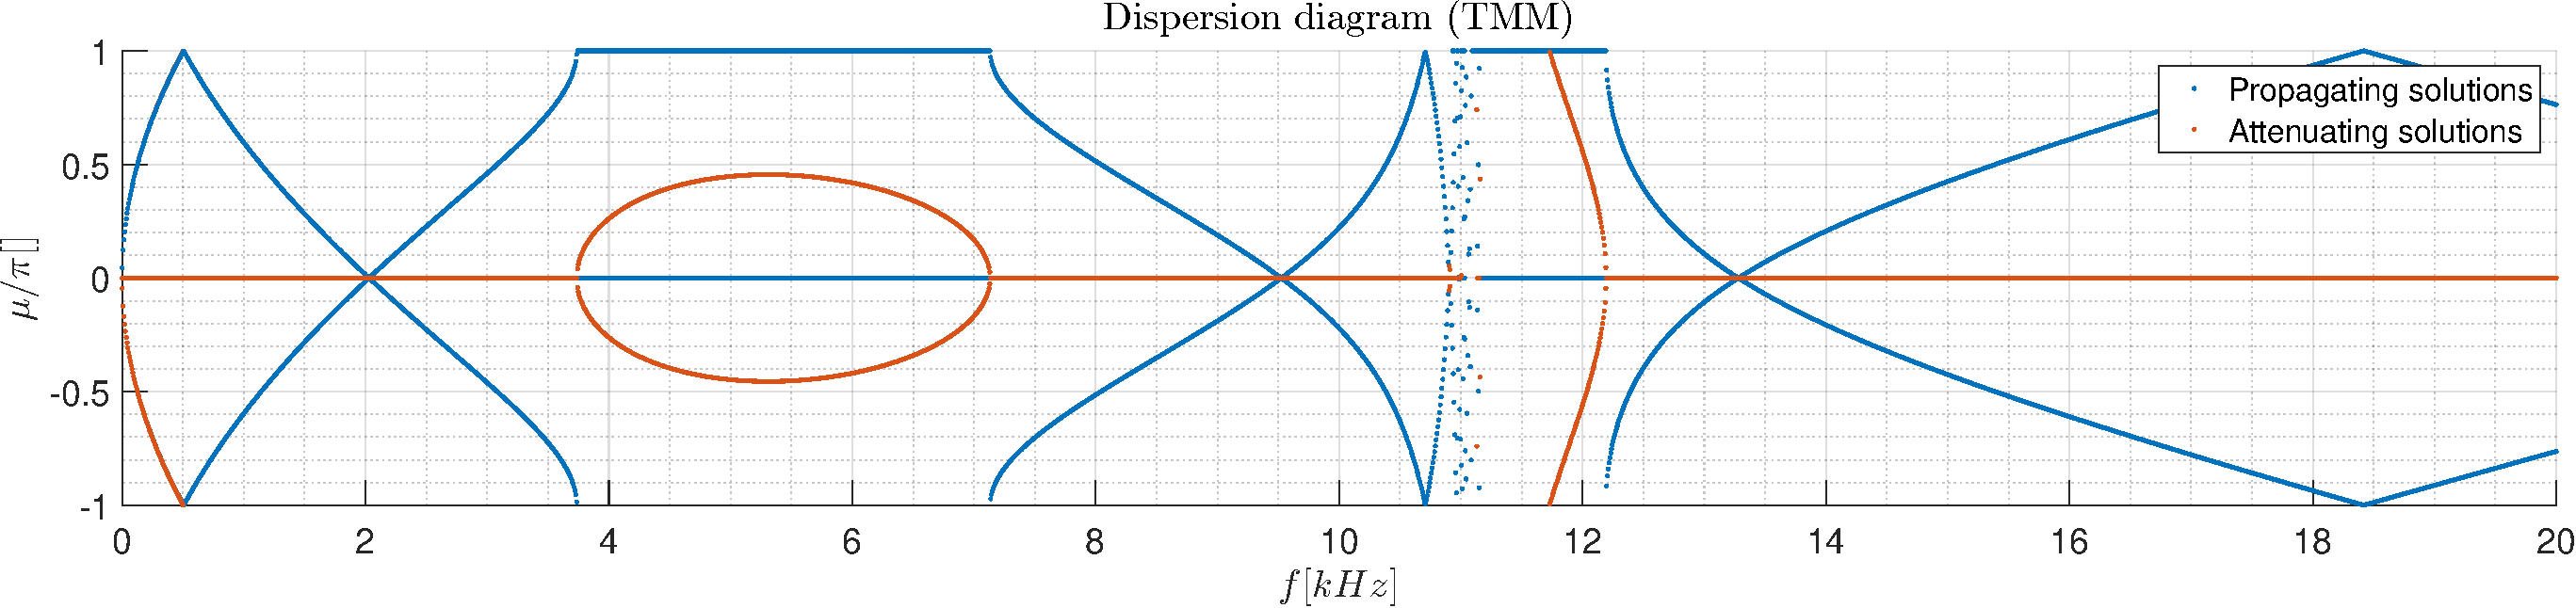
\includegraphics[width=\textwidth]{./img/MATLAB/TMM_ON-ON-ON_RLC_R0_L0.03_CInf.pdf}
    \caption{RLC shunt circuit with $R = 0 \Omega$, $L = 0.03 H$, and $C = \infty F$.}
    \label{fig:TMM_ON-ON-ON_RLC_R0_L0.03_CInf.pdf}
\end{figure}

\begin{figure}[H]
    \centering
    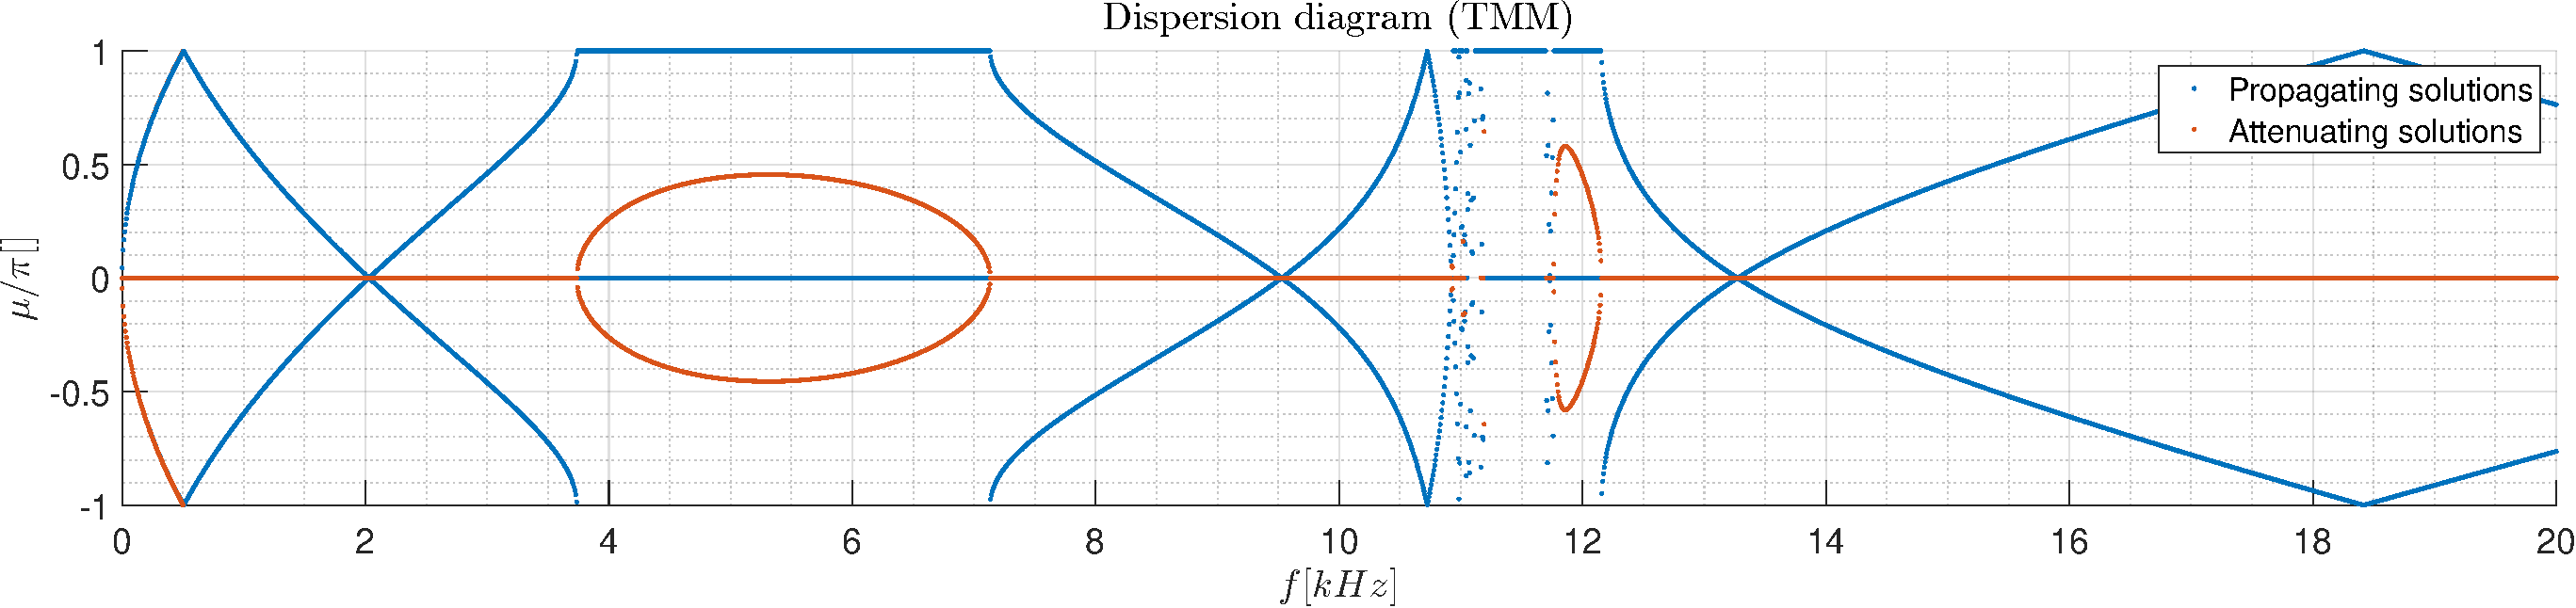
\includegraphics[width=\textwidth]{./img/MATLAB/TMM_ON-ON-ON_RLC_R50_L0.03_CInf.pdf}
    \caption{RLC shunt circuit with $R = 50 \Omega$, $L = 0.03 H$, and $C = \infty F$.}
    \label{fig:TMM_ON-ON-ON_RLC_R50_L0.03_CInf.pdf}
\end{figure}

\begin{figure}[H]
    \centering
    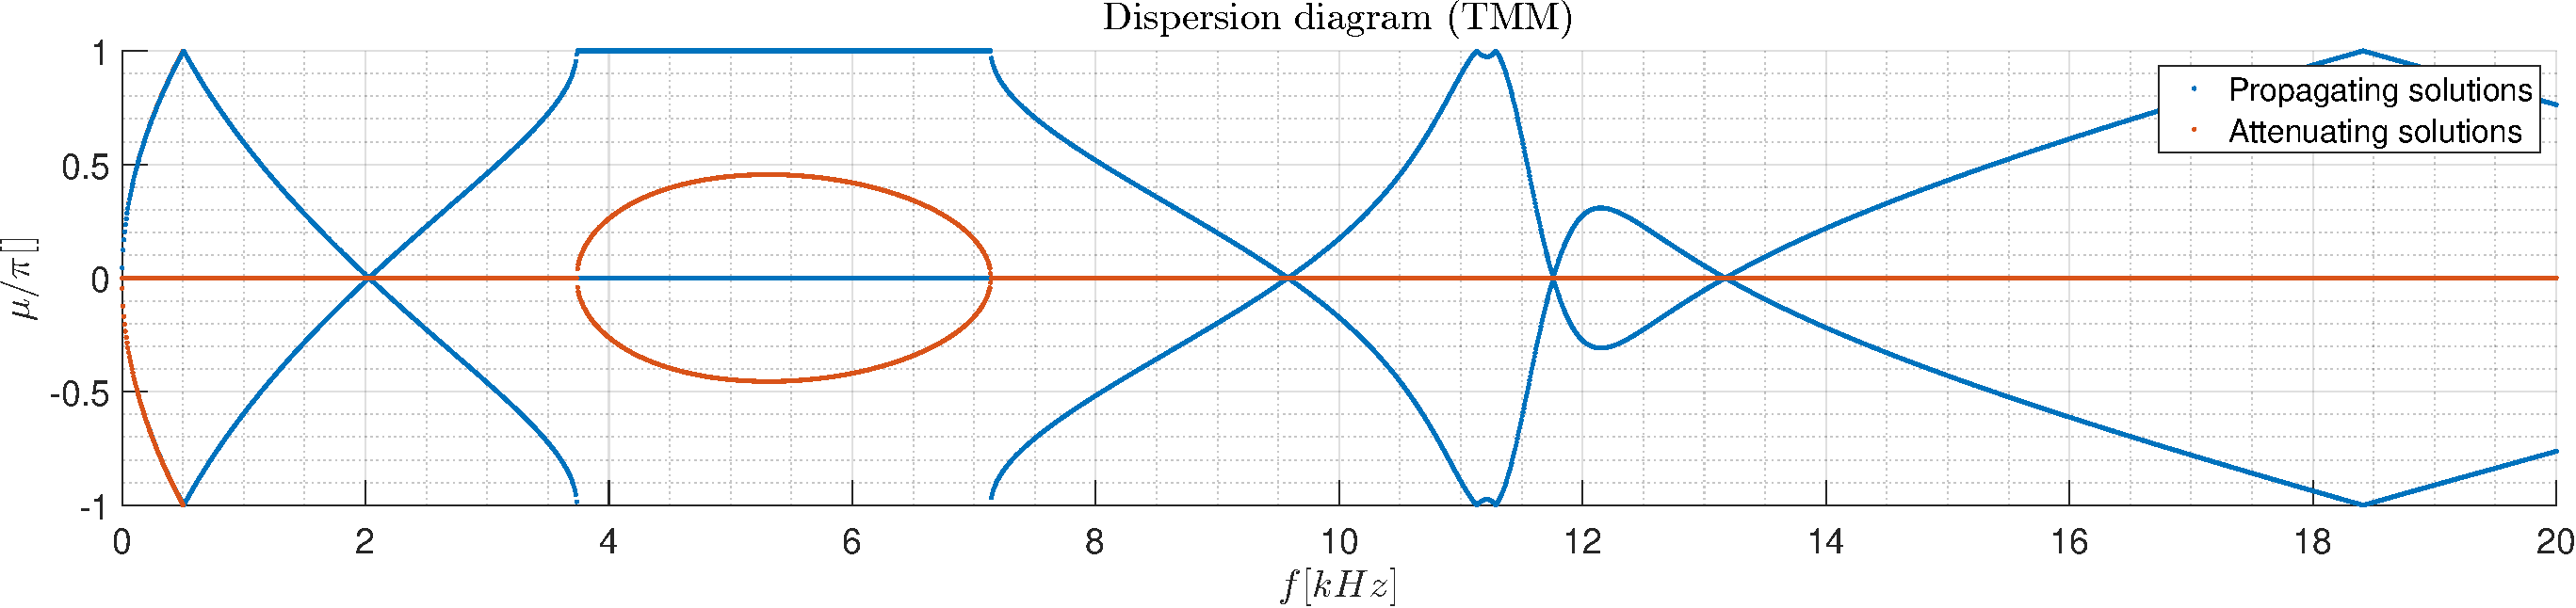
\includegraphics[width=\textwidth]{./img/MATLAB/TMM_ON-ON-ON_RLC_R200_L0.03_CInf.pdf}
    \caption{RLC shunt circuit with $R = 200 \Omega$, $L = 0.03 H$, and $C = \infty F$.}
    \label{fig:TMM_ON-ON-ON_RLC_R200_L0.03_CInf.pdf}
\end{figure}

\begin{figure}[H]
    \centering
    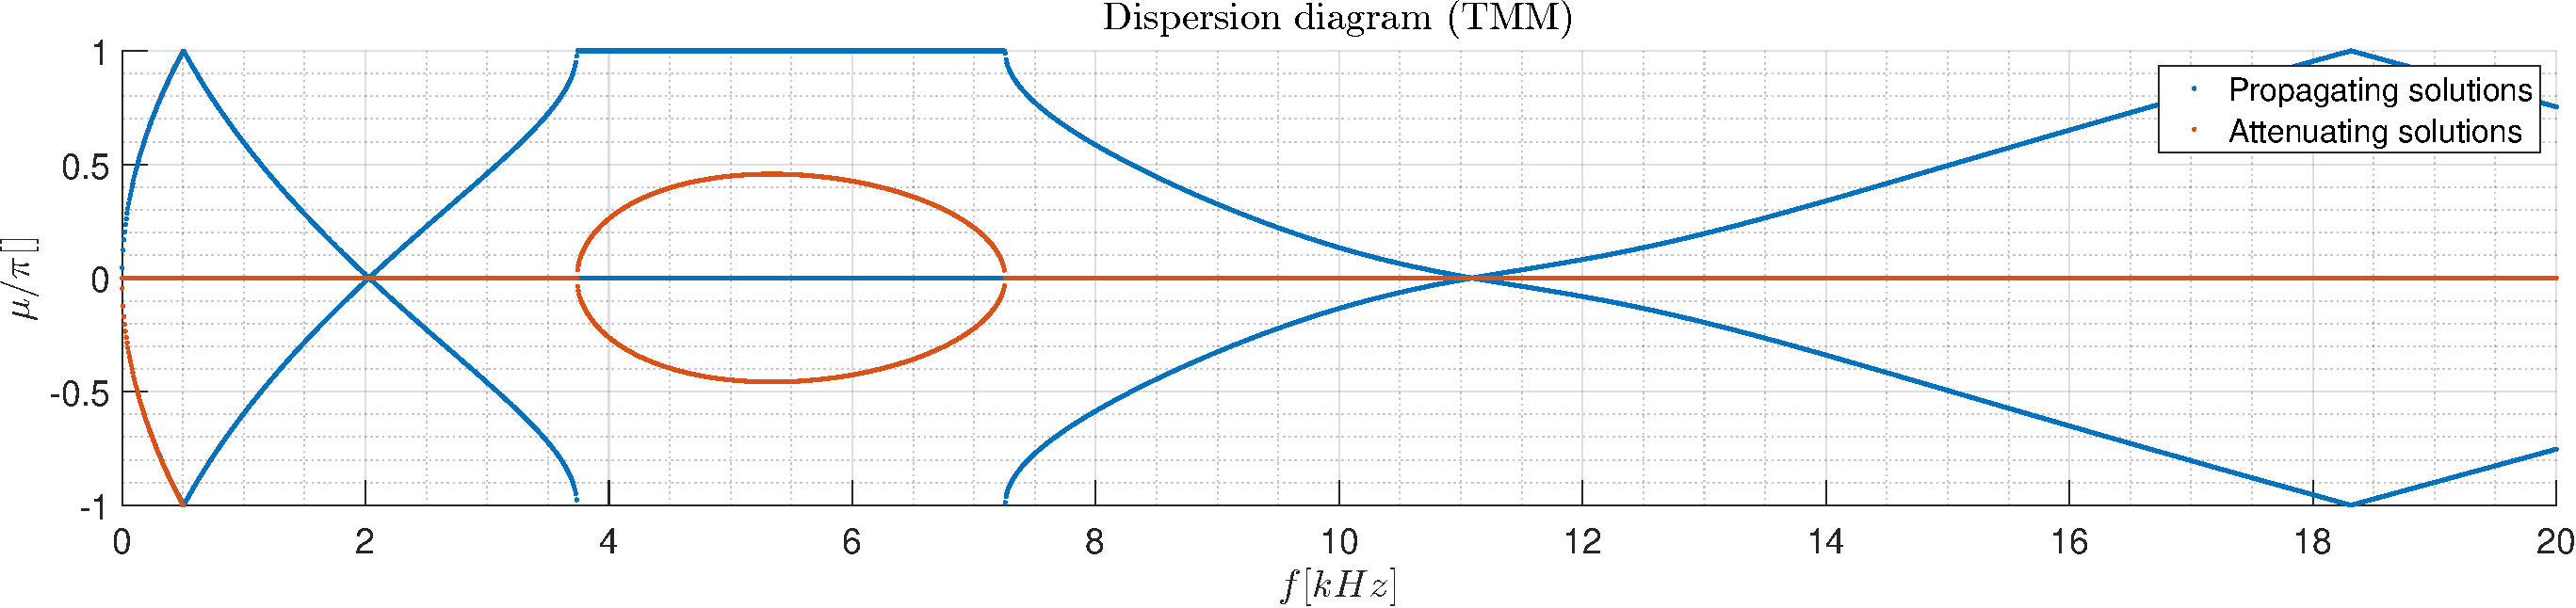
\includegraphics[width=\textwidth]{./img/MATLAB/TMM_ON-ON-ON_RLC_R1000_L0.03_CInf.pdf}
    \caption{RLC shunt circuit with $R = 1000 \Omega$, $L = 0.03 H$, and $C = \infty F$.}
    \label{fig:TMM_ON-ON-ON_RLC_R1000_L0.03_CInf.pdf}
\end{figure}

Based also on Figure \ref{fig:Y_SU_Resistive-Inductive_shunt_circuit.pdf}, it's possible to observe that at low frequencies the system behaves as in the short circuit case, while at higher frequencies the system behaves as in the open circuit case, similarly to the purely inductive case.

However, the main difference is that the resistive element $R$ acts as a damping factor, which can be used to control the width and the depth of the band-gap.
This phenomenon is clearly visible in the dispersion relation plots, where the central position of the band-gap remains the same (governed by $L$ only), while the attenuation level decreases with increasing $R$.
For high values of $R$, regardless of the value of $L$, the band-gap can be completely suppressed.



\paragraph{$RC_N$ shunt circuit}

In the case of a resistive-(negative) capacitive shunt circuit, the impedance of the shunt circuit is given by $Z_{su} = R - \frac{1}{sC_N}$.
The equation for the mechanical admittance of the piezoelectric patch is:

\begin{equation}
    Y^{SU} = Y_1^D \left( 1 - \frac{k_{31}^2}{1 - C_p^S \frac{1}{C_N} - s C_p^S R} \right)
    \label{eq:mechanical_admittance_RC_shunt}
\end{equation}

For the analysis, three values of $C_N$ are considered while $R$ and $L$ are kept constant at $1000 \Omega$ and $0H$, respectively.

\begin{table}[H]
    \centering
    \begin{tabular}{|c|c|c|}
        \hline
        $R$ [$\Omega$] & $L$ [H] & $C_N$ [F] \\
        \hline
        1000           & 0       & 30e-9     \\
        1000           & 0       & 7e-9      \\
        1000           & 0       & 5e-9      \\
        \hline
    \end{tabular}
    \caption{Values of $R$, $L$, and $C_N$ for the resistive-(negative) capacitive shunt circuit.}
    \label{tab:RLC_N_values_RC_case}
\end{table}

One can also visualize the effect of the capacitive element on the system by plotting $Y^{SU}$ for the different values of $C_N$.

\begin{figure}[H]
    \centering
    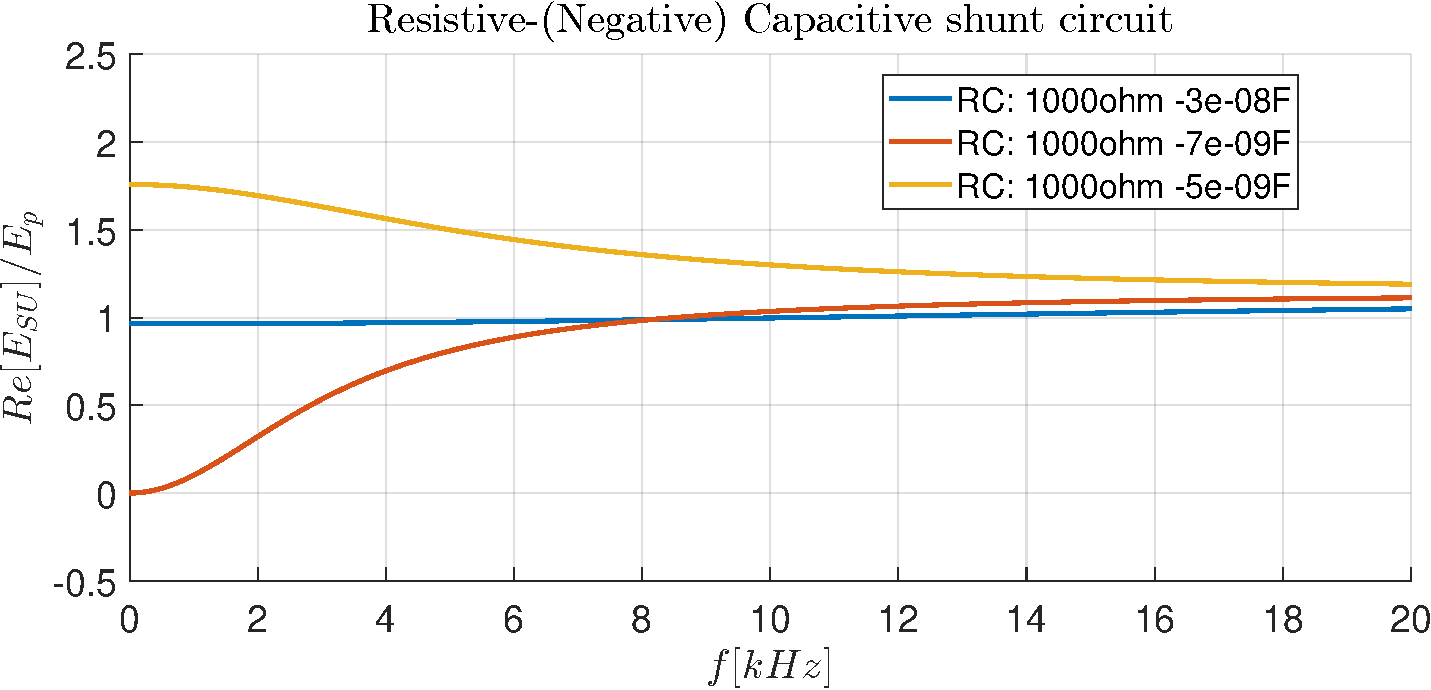
\includegraphics[width=0.6\textwidth]{./img/MATLAB/Y_SU_Resistive-(Negative) Capacitive shunt circuit.pdf}
    \caption{Analysis of $Y^{SU}$ for the resistive-(negative) capacitive shunt circuit.}
    \label{fig:Y_SU_Resistive-(Negative)_Capacitive_shunt_circuit.pdf}
\end{figure}

Instead, the dispersion relation of the system are shown in the figures below.

\begin{figure}[H]
    \centering
    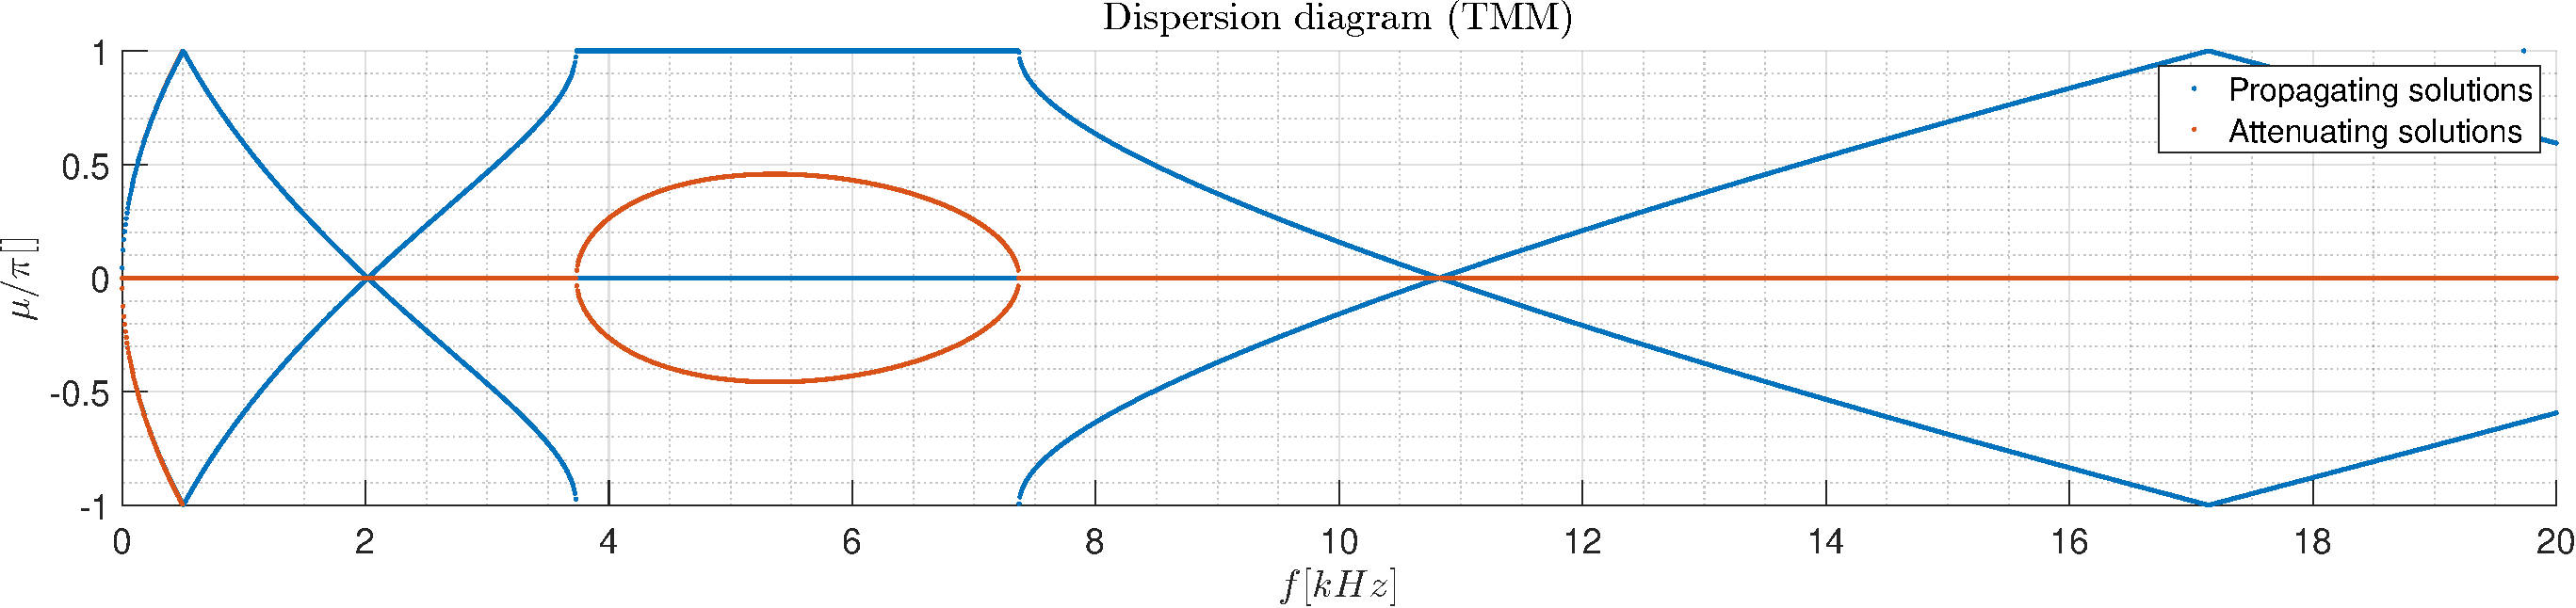
\includegraphics[width=\textwidth]{./img/MATLAB/TMM_ON-ON-ON_RLC_R1000_L0_C-3e-08.pdf}
    \caption{RLC shunt circuit with $R = 1000 \Omega$, $L = 0 H$, and $C = -30 nF$.}
    \label{fig:TMM_ON-ON-ON_RLC_R1000_L0_C-30e-09.pdf}
\end{figure}

\begin{figure}[H]
    \centering
    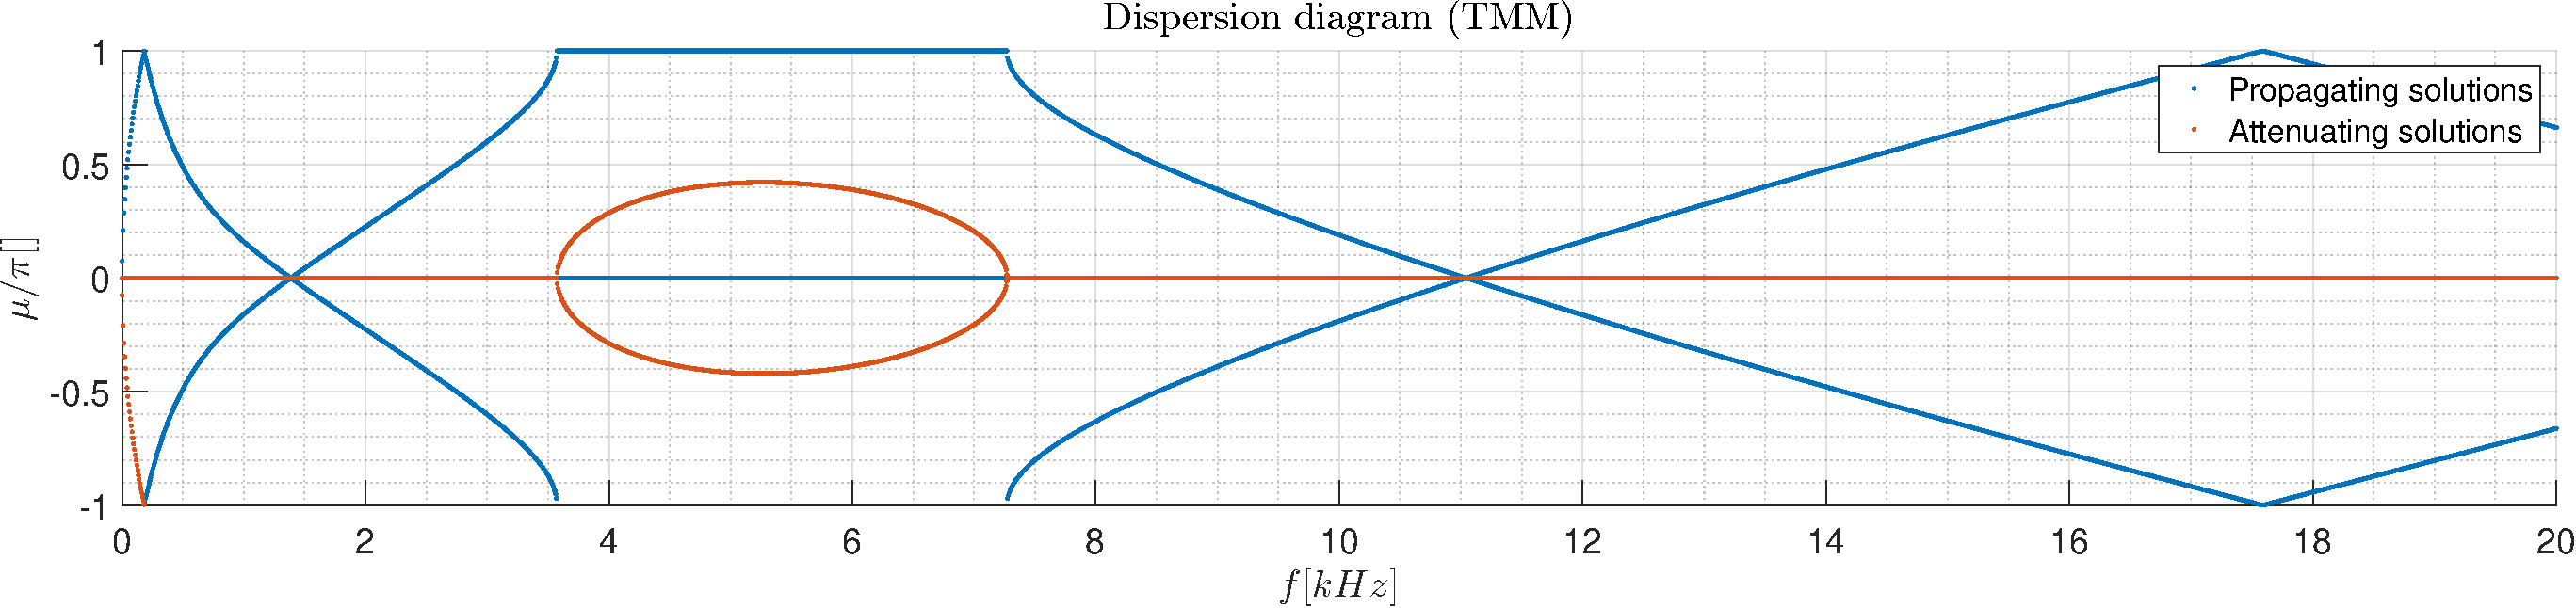
\includegraphics[width=\textwidth]{./img/MATLAB/TMM_ON-ON-ON_RLC_R1000_L0_C-7e-09.pdf}
    \caption{RLC shunt circuit with $R = 1000 \Omega$, $L = 0 H$, and $C = -7 nF$.}
    \label{fig:TMM_ON-ON-ON_RLC_R1000_L0_C-7e-09.pdf}
\end{figure}

\begin{figure}[H]
    \centering
    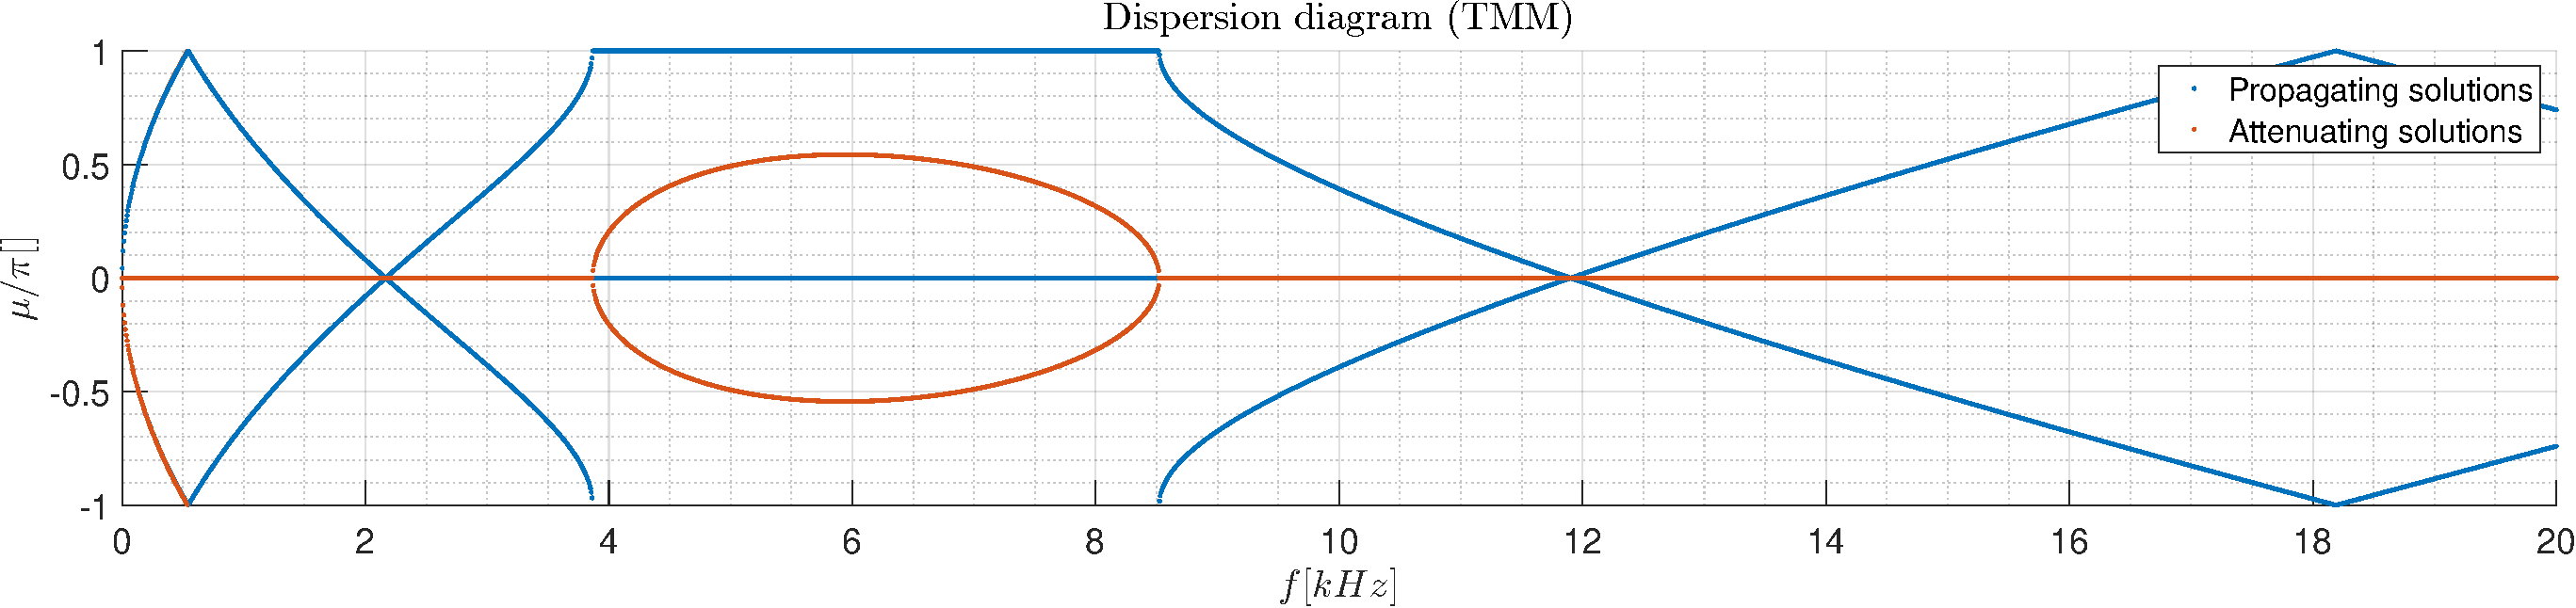
\includegraphics[width=\textwidth]{./img/MATLAB/TMM_ON-ON-ON_RLC_R1000_L0_C-5e-09.pdf}
    \caption{RLC shunt circuit with $R = 1000 \Omega$, $L = 0 H$, and $C = -5 nF$.}
    \label{fig:TMM_ON-ON-ON_RLC_R1000_L0_C-5e-09.pdf}
\end{figure}

The effect of the negative capacitance is to shift the band-gap frequencies.
Depending on the sign of $1 - C_p^S \frac{1}{C_N}$, the band-gap can be shifted to higher (negative sign) or lower (positive sign) frequencies.
This effect can be used to tune the band-gap to a desired frequency range.

Notice however that the introduction of a negative capacitance can lead to instability issues, as the system can become underdamped.
Not all the configurations shown in the figures above are in fact stable, the purpose of this analysis is to show the effect of the negative capacitance on the system's band-gap and not to provide a stable configuration.





\subsection{Stability analysis}
\label{subsec:stability_analysis}

As introduced at the beginning this section, a shunting circuit can be either passive or active.
While passive shunts are stable by definition (conservation of energy), active shunts can introduce instabilities in the system.

In particular, considering piezoelectric patches connected to a shunting circuts, two types of instabilities can be introduced:

\begin{itemize}
    \item \textbf{Mechanical instability}: the equivalent stiffness of the piezoelectric patch become negative;
    \item \textbf{Electrical instability}: the equivalent capacitance of the electrical circuit becomes negative.
\end{itemize}

For the sake of simplicity, we consider here only the case of the purely capacitance shunting circuit, with a series connection between the piezoelectric patch and the shunt capacitor (similar to the one shown in Figure \ref{fig:shunt_layouts} (a)).


\subsubsection{$C_N$ shunting circuit}
\label{subsubsec:stability_analysis_negative_capacitance}

As already discussed, the negative capacitance shunting circuit is a particular case of active shunt circuit that can be implemented via OP-AMPs as explained at the beginning of the section.

In this case, considering $Z_{SU} = -\frac{1}{sC_N}$, the mechanical admittance of the piezoelectric patch can be written as:

\begin{equation}
    Y^{SU} = Y_1^D \left( 1 - \frac{k_{31}^2}{1 - C_p^S \frac{1}{C_N}} \right)
\end{equation}

If we consider the ideal case for the shunting circuit, we have already shown in Equation \ref{eq:negative_capacitance_ideal} that the value of $C_N$ doesn't depend on the value of $s = j\omega$.
This means that instability properties (at least in the ideal case) are not frequency-dependent, but rather depends only on the selected value of $C_N$.

In Figure \ref{fig:stability_analysis_negative_capacitance} we show the normalized mechanical admittance of the piezoelectric patch function of the normalized capacitance of the shunting circuit.

\begin{figure}[H]
    \centering
    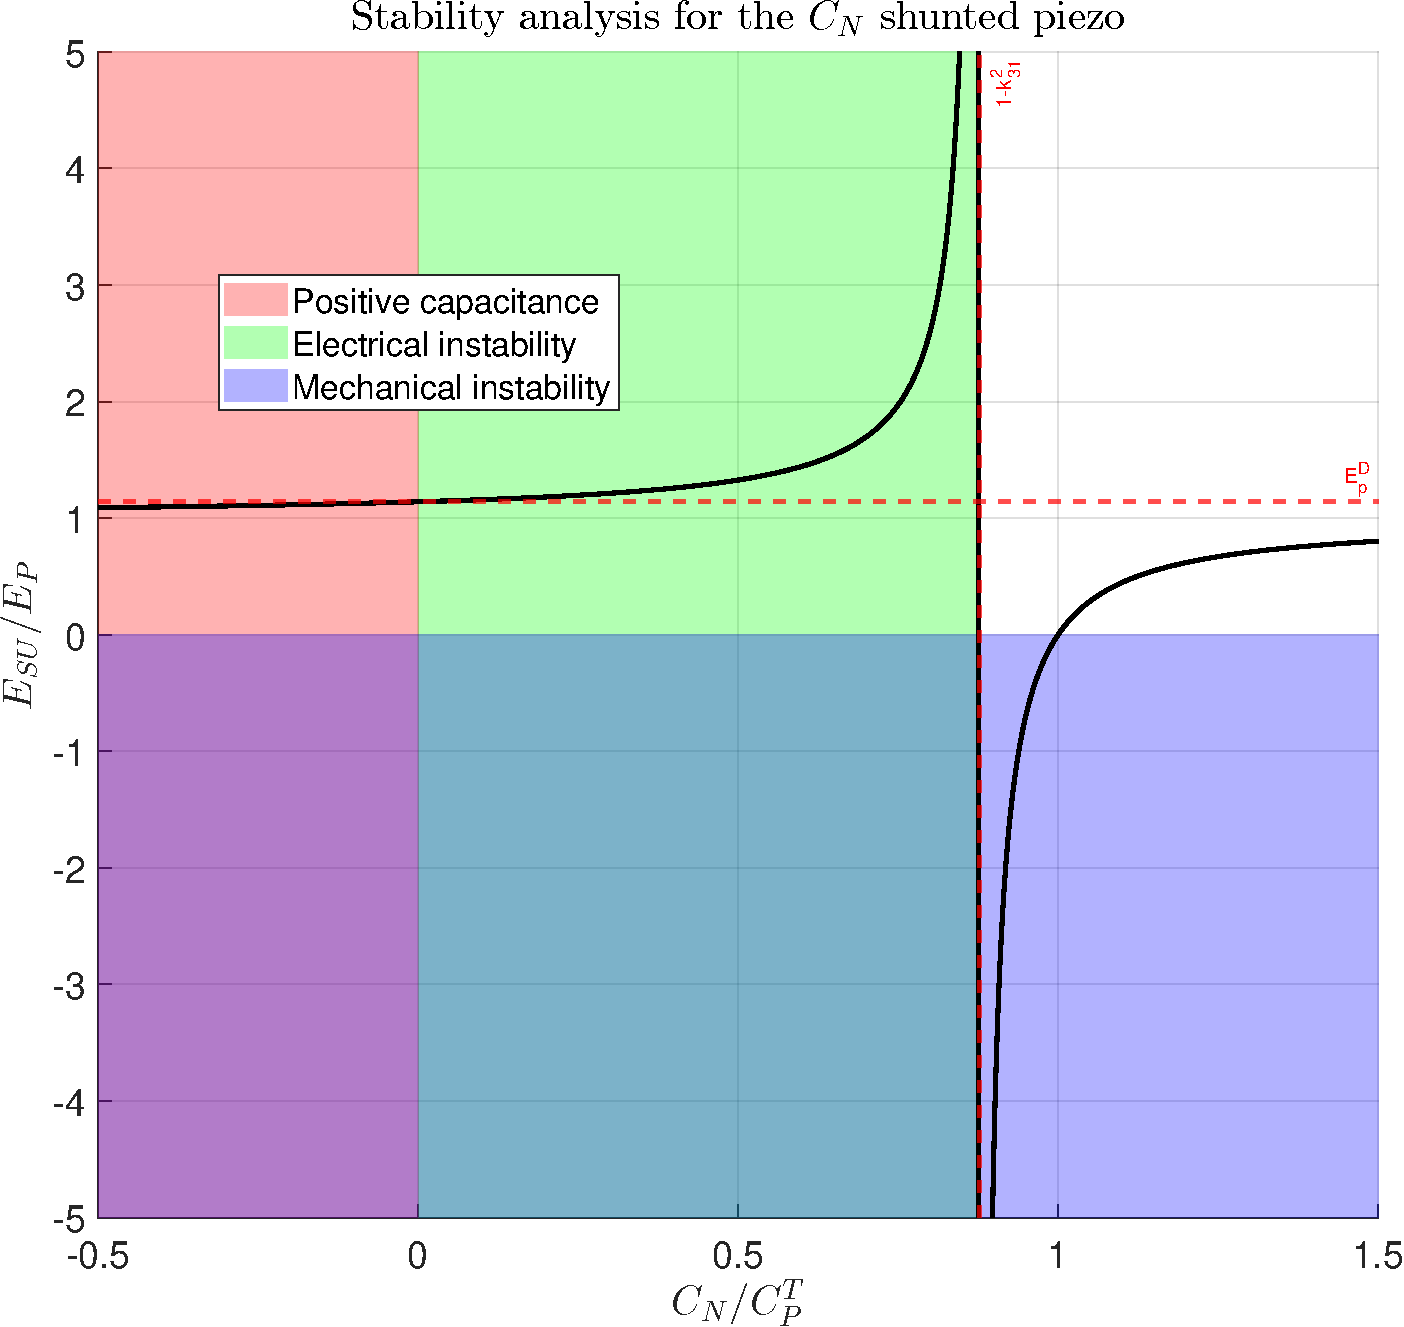
\includegraphics[width=0.5\textwidth]{./img/MATLAB/Stability_analysis_C_N.pdf}
    \caption{Stability analysis of the negative capacitance shunting circuit.}
    \label{fig:stability_analysis_negative_capacitance}
\end{figure}

The colored regions in the plot highlight the regions of mechanical instability (blue) and electrical instability (green).
The red region instead highlights the region where $C_N$ is negative, which means having positive capacitance in the shunting circuit ($C_{eq} = -C_N$).


\paragraph{Mechanical instability}

The mechanical instability region is defined by the condition:

\begin{equation}
    Y^{SU} < 0 \rightarrow 1 - \frac{k_{31}^2}{1 - C_p^S \frac{1}{C_N}} < 0
\end{equation}


\paragraph{Electrical instability}

The electrical instability region is defined by the condition:

\begin{equation}
    C_{tot} = \left( \frac{1}{C_p^T} - \frac{1}{C_N} \right)^{-1} < 0
\end{equation}

Re-arranging the terms, we have:

\begin{equation}
    C_N < C_p^T
\end{equation}




\section{Experimental approach}
\label{sec:experimental_approach}

As shown from a theoretical point of view in Section \ref{sec:analysis_shunted_piezo}, it's possible to control the band-gaps of a beam by means of shunted piezoelectric patches.
Experimental validation has also been performed in this sense and is presented in this section.

At first, the experimental setup is described, highlighting the configuration used for the piezoelectric patches and the shunt circuits.
Then, the experimental data are presented together with the theoretical predictions obtained through the numerical methods presented in Section \ref{subsec:numerical_methods_for_wave_propagation_analysis}.

At first, the space-only modulation is considered, and the tools used for the analysis are the Transfer Matrix Method (TMM) and the Plane Wave Expansion Method (PWEM).
\texttt{Comsol Multiphysics} is also adoperated to validate both the numerical methods results and the experimental data.
Then, the space-time modulation is considered, and the nonreciprocal behavior is highlighted showing that the experimental results are in agreement with the theoretical predictions obtained from PWEM.

\subsection{Setup}
\label{subsec:experimental_setup}

As already anticipated, material property modulation is achieved by means of shunted piezoelectric patches.
Figure \ref{fig:experimental_setup} illustrates the experimental setup, highlighting the placement of the piezoelectric patches and the shunt circuits.

\begin{figure}[H]
    \centering
    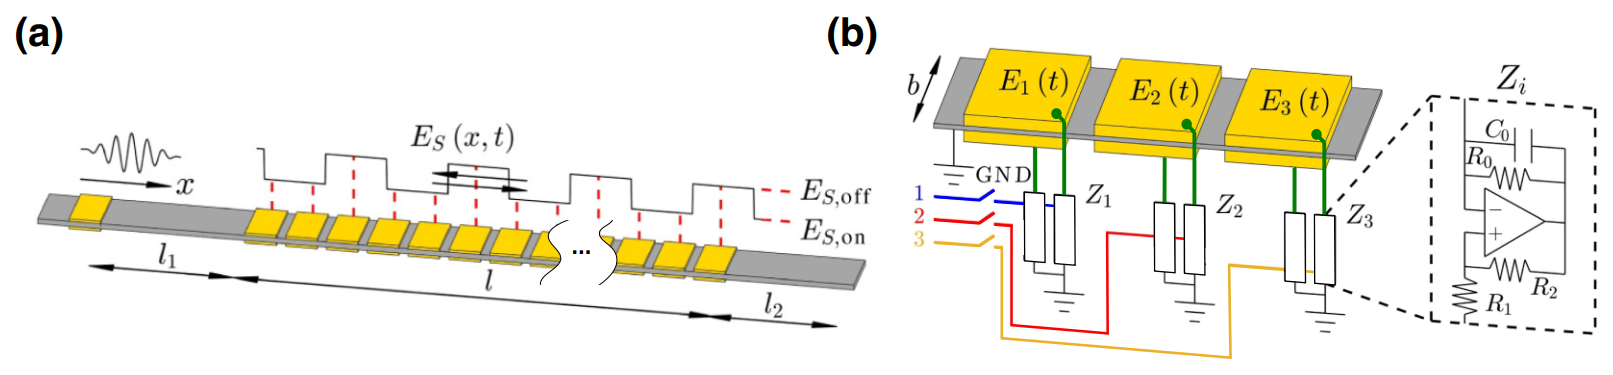
\includegraphics[width=0.9\textwidth]{./img/experimental_setup_scheme.png}
    \caption{Schematic of the experimental setup.}
    \label{fig:experimental_setup}
\end{figure}

In particular, Figure \ref{fig:experimental_setup} (a) depicts the electromechanical beam, including the excitation patch (responsible for generating the travelling wave signal) and the active domain containing the array of piezoelectric patches.
Figure \ref{fig:experimental_setup} (b) provides a close-up view of the unit spatiotemporal (ST) cell, consisting of three piezoelectric patches and the corresponding $C_N$ type shunt circuits.
Active modualtion is achieved by toggling switches that control the connection between the power supply and operational amplifiers.

The host beam consists of an aluminum substrate with a cross-section of $20 mm \times 1 mm$ and a total length of $2400 mm$.
An array of piezoelectric patches, spaced $2 mm$ apart, is positioned at $l_1 = 690 mm$ and $l_2 = 1134 mm$ from the beam's left and right boundaries, respectively.
This choice of placement minimizes boundary reflections, further mitigated by the use of absorbing boundary layers composed of mastic tape.

The active piezoelectric region, spanning $576 mm$, consists of $24$ pairs of piezoelectric patches with dimensions $20 mm \times 22 mm \times 1 mm$.
These patches are bonded on opposite surfaces of the beam and connected to a total of $48$ negative capacitance shunt circuits.
When the circuit is closed, the effective stiffness of the beam section is reduced (see Equation \ref{eq:weighted_average_mechanical_properties}).

The out-of-plane velocity field along the beam's length is measured using a Polytec 3D laser Doppler vibrometer (SLDV).

In Table \ref{tab:experimental_setup_parameters}, the main parameters of the experimental setup are summarized.

\begin{table}[H]

    \centering

    \begin{tabular}{|l|c|c|c|}
        \hline
        \textbf{Parameter}                 & \textbf{Symbol} & \textbf{Value} & \textbf{Units} \\
        \hline
        Beam Young's modulus               & $Y_b$           & $69$           & $GPa$          \\
        Beam density                       & $\rho_b$        & $2700$         & $kg/m^3$       \\
        \hline
        Piezoelectric Young's modulus      & $Y_1^E$         & $62$           & $GPa$          \\
        Piezoelectric capacitance          & $C_T$           & $7.0$          & $nF$           \\
        Piezoelectric coupling coefficient & $k_{31}$        & $0.351$        & -              \\
        Piezoelectric density              & $\rho$          & $7900$         & $kg/m^3$       \\
        \hline
        Shunt capacitance                  & $C_0$           & $4.4$          & $nF$           \\
        Shunt bias resistance              & $R_0$           & $1.0$          & $M\Omega$      \\
        Shunt resistance                   & $R_1$           & $7.5$          & $k\Omega$      \\
        Shunt resistance                   & $R_2$           & $13.7$         & $k\Omega$      \\
        \hline
    \end{tabular}

    \caption{Main parameters of the experimental setup.}
    \label{tab:experimental_setup_parameters}

\end{table}
\subsection{Space-Only Modulation}
\label{subsec:space_only_modulation}

In the case of space-only modulation, a given pair of piezoelectric patches can be either in the short-circuit or open-circuit state.
For simplicity, we will refer to these states as ON and OFF, respectively.

Considering the ST cell as composed by three pairs of piezoelectric patches, three different configurations are analyzed:

\begin{itemize}
    \item OFF-OFF-OFF: all the shunt circuits are open;
    \item ON-ON-ON: all the shunt circuits are closed;
    \item OFF-OFF-ON: only the last shunt circuit is closed.
\end{itemize}

The mechanical properties of the system are computed so to obtain $EJ(x)$ and $\rho A(x)$, which are then used by the numerical methods to compute the dispersion diagram of the system.
In the following, the results of the numerical simulations are compared with the experimental data.

Both the TMM and PWEM are expected to exhibit some discrepancies with the experimental data at higher frequencies due to the hypothesis made in the theoretical model.
The Euler-Bernoulli beam theory that has been used in the theoretical model, is known to be a good approximation only for low-frequency excitations and small deformations.
Timošenko beam theory could have been a better choice, but it would have made the theoretical model more complex and the numerical simulations more computationally expensive.

Moreover, for the PWEM, a number of space and time harmonics equal to $P = 40$ and $Q = 1$ are considered, respectively.
The relative low number of space harmonics is expected to introduce some additional discrepancies with the experimental data, especially at higher frequencies.

\texttt{Comsol Multiphysics} is used as a valid reference to validate the experimental results given that internal losses and higher order modes are taken into account into its numerical solvers.


\paragraph{OFF-OFF-OFF}

The first case considered is the OFF-OFF-OFF configuration, where all the shunt circuits are open.
In this case, based on Equation \ref{eq:mechanical_admittance_shunted_piezoelectric_patch}, the piezo's mechanical admittance is given by:

\begin{equation}
    Y^{SU} = Y_1^D
\end{equation}

Figure \ref{fig:space_only_off_off_off}, shows the PWEM and experimental results, while the comparison between the TMM and Comsol Multiphysics is shown in Figure \ref{fig:space_only_off_off_off_comsol}.

\begin{figure}[H]
    \centering
    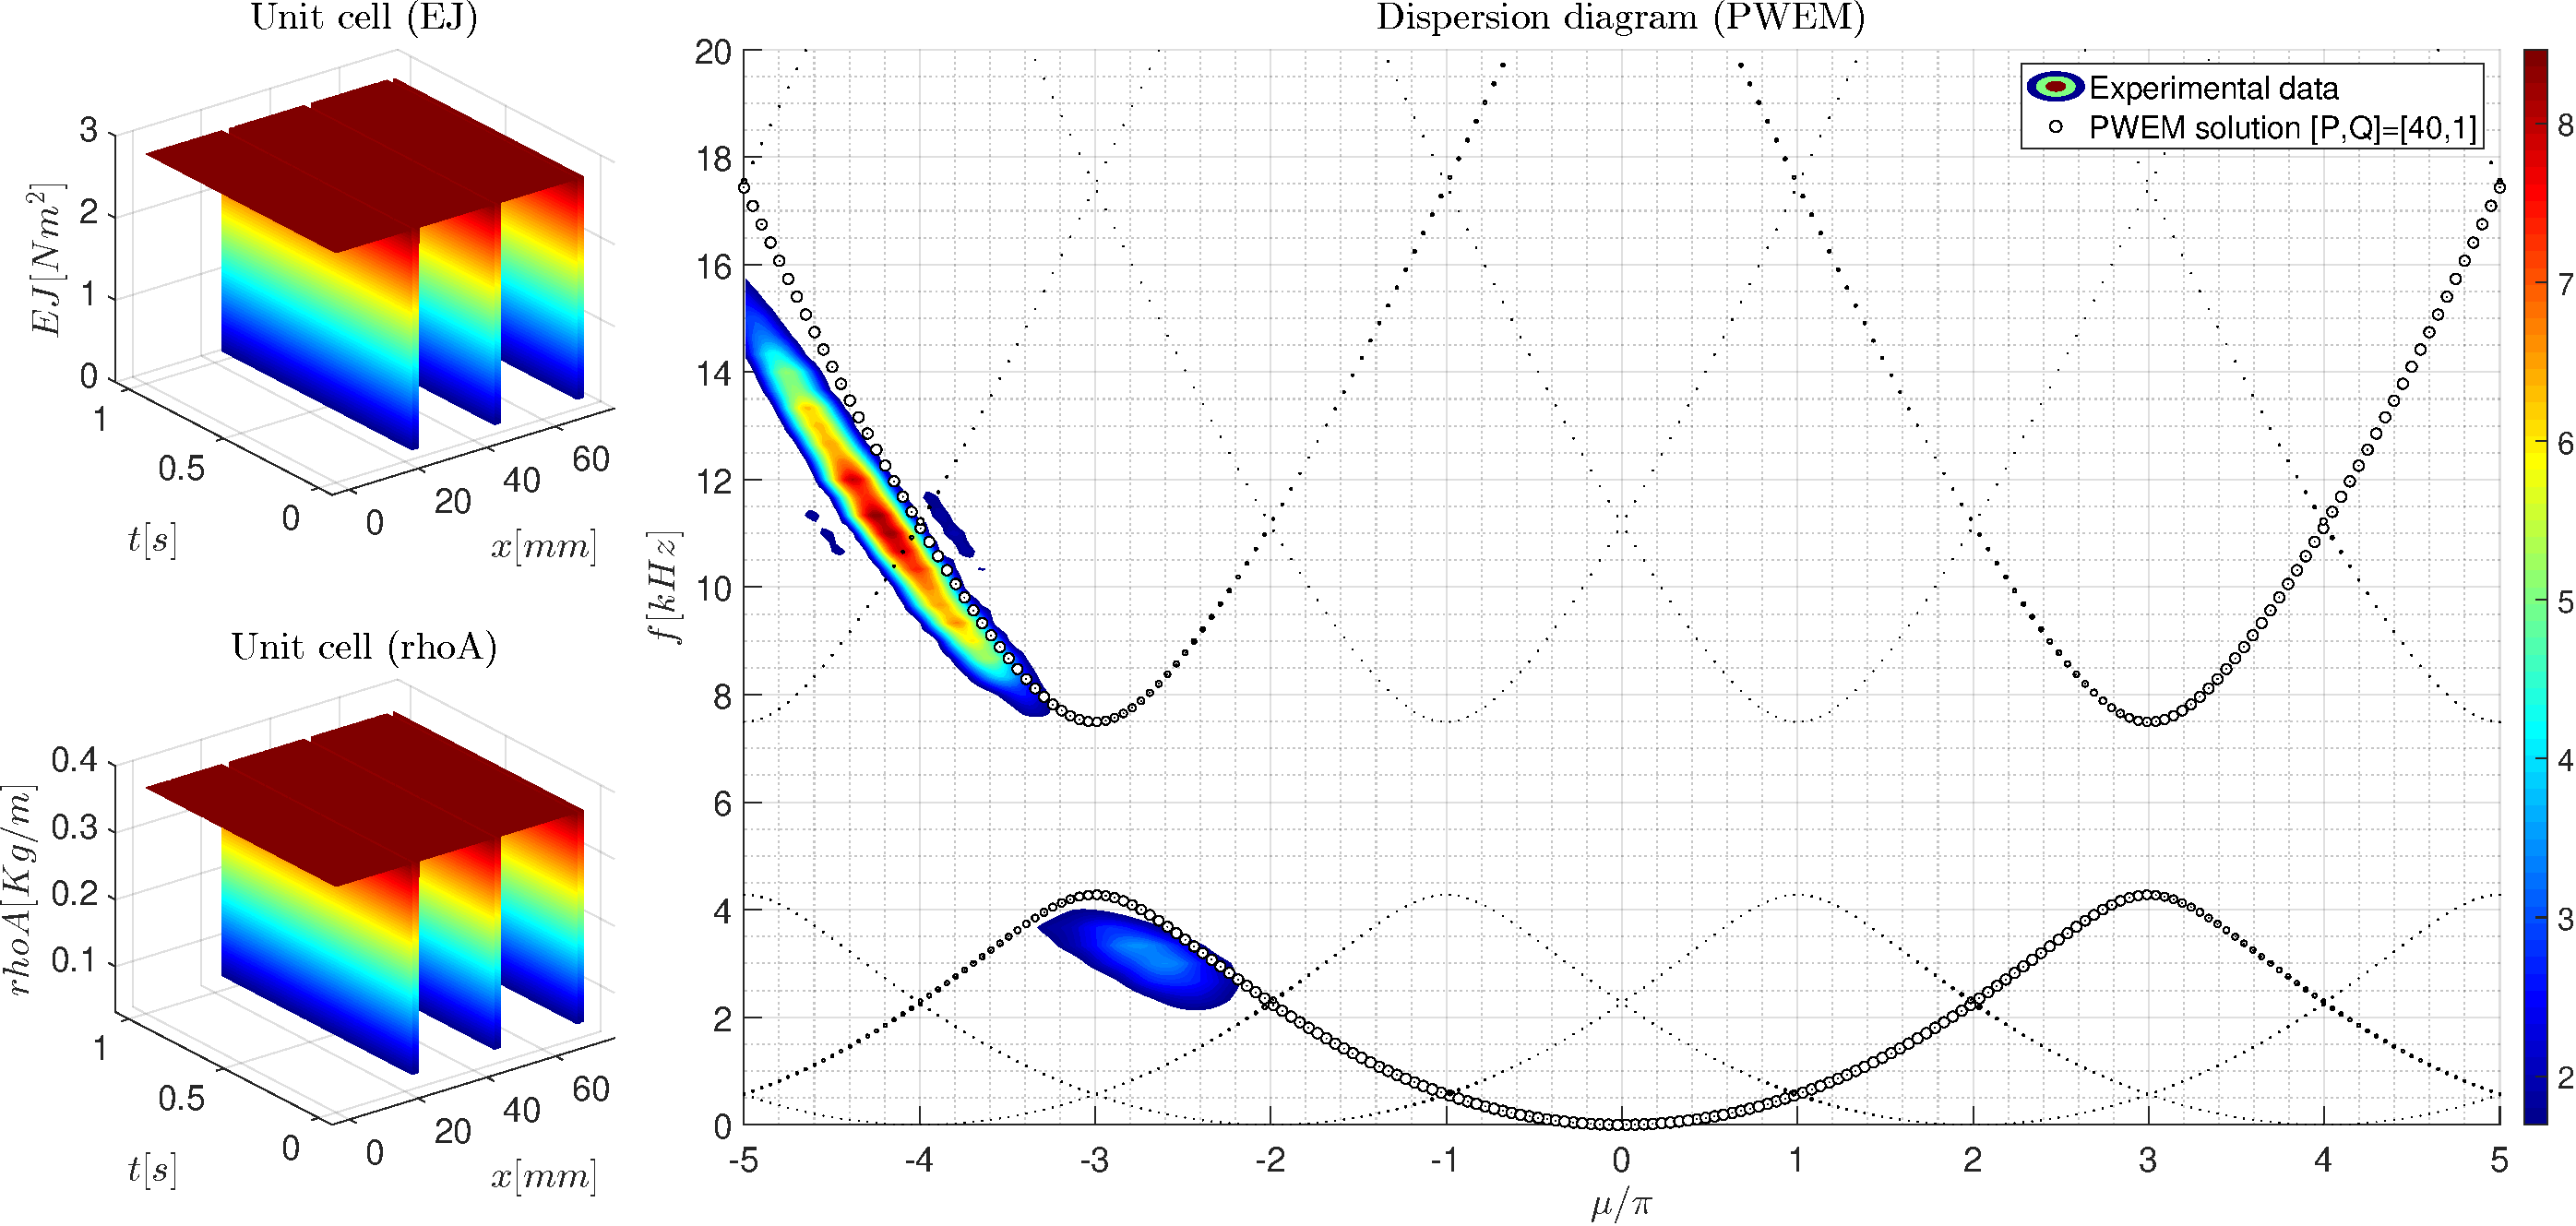
\includegraphics[width=\textwidth]{./img/MATLAB/PWEM_EXP OFF-OFF-OFF @0kHz.pdf}
    \caption{Band structure for the OFF-OFF-OFF configuration.}
    \label{fig:space_only_off_off_off}
\end{figure}

\begin{figure}[H]
    \centering
    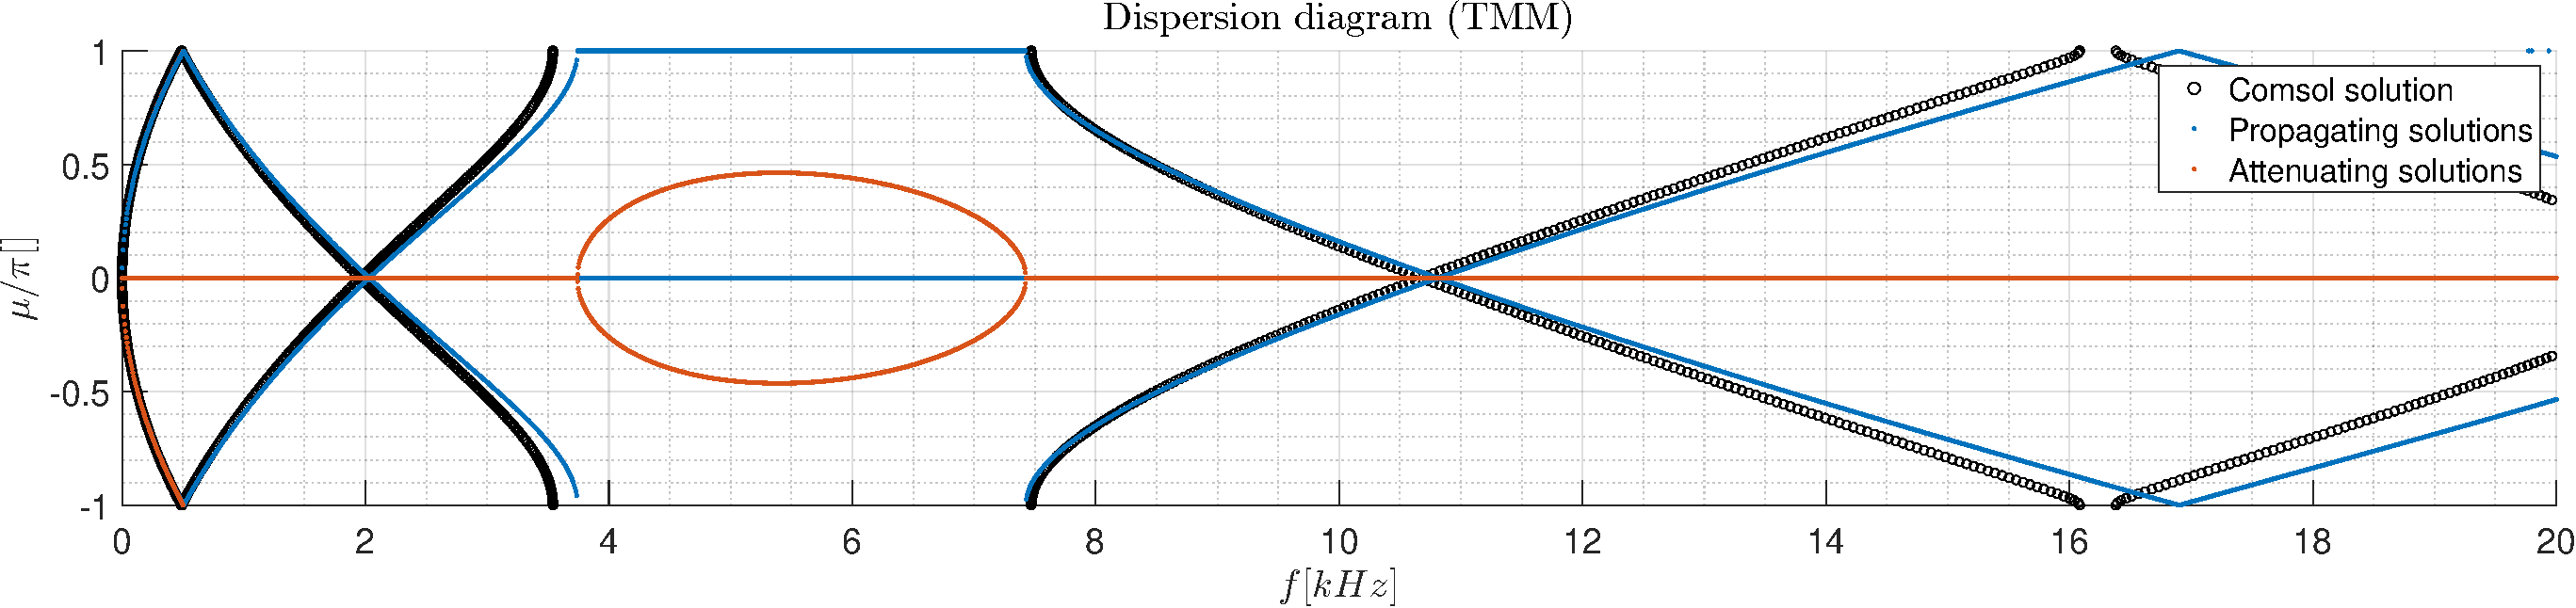
\includegraphics[width=\textwidth]{./img/MATLAB/TMM_COMSOL OFF-OFF-OFF @0kHz.pdf}
    \caption{Comparison between TMM and Comsol Multiphysics for the OFF-OFF-OFF configuration.}
    \label{fig:space_only_off_off_off_comsol}
\end{figure}

In the above figures, what has been suggested with the introductory considerations is confirmed.
Both the TMM and PWEM exhibit some discrepancies with the experimental data at higher frequencies.
However, their results are still in good agreement with the experimental data, being able to predict the band-gap position.

From the comparison between the TMM and Comsol Multiphysics, it can be seen that the TMM method underestimate the stiffness of the beam at higher frequencies, causing an upper shift of the dispersion diagram with respect to both the experimental data and the Comsol Multiphysics results.
Under the hypothesis that this offset is due to the Euler-Bernoulli assumption, we can state that the model can be considered valid for the analysis of the system.

In the case of the OFF-OFF-OFF configuration, the band gap of the structure is found at:

\begin{equation}
    f_{BG}^{OFF-OFF-OFF} = [3.8, 7.5] kHz
\end{equation}



\paragraph{ON-ON-ON}

The second case considered is the ON-ON-ON configuration, where all the shunt circuits are in the short-circuit state.
In this case, the piezo's mechanical admittance is given by:

\begin{equation}
    Y^{SU} = Y_1^E
\end{equation}

Figure \ref{fig:space_only_on_on_on}, shows the PWEM and experimental results, while the comparison between the TMM and Comsol Multiphysics is shown in Figure \ref{fig:space_only_on_on_on_comsol}.

\begin{figure}[H]
    \centering
    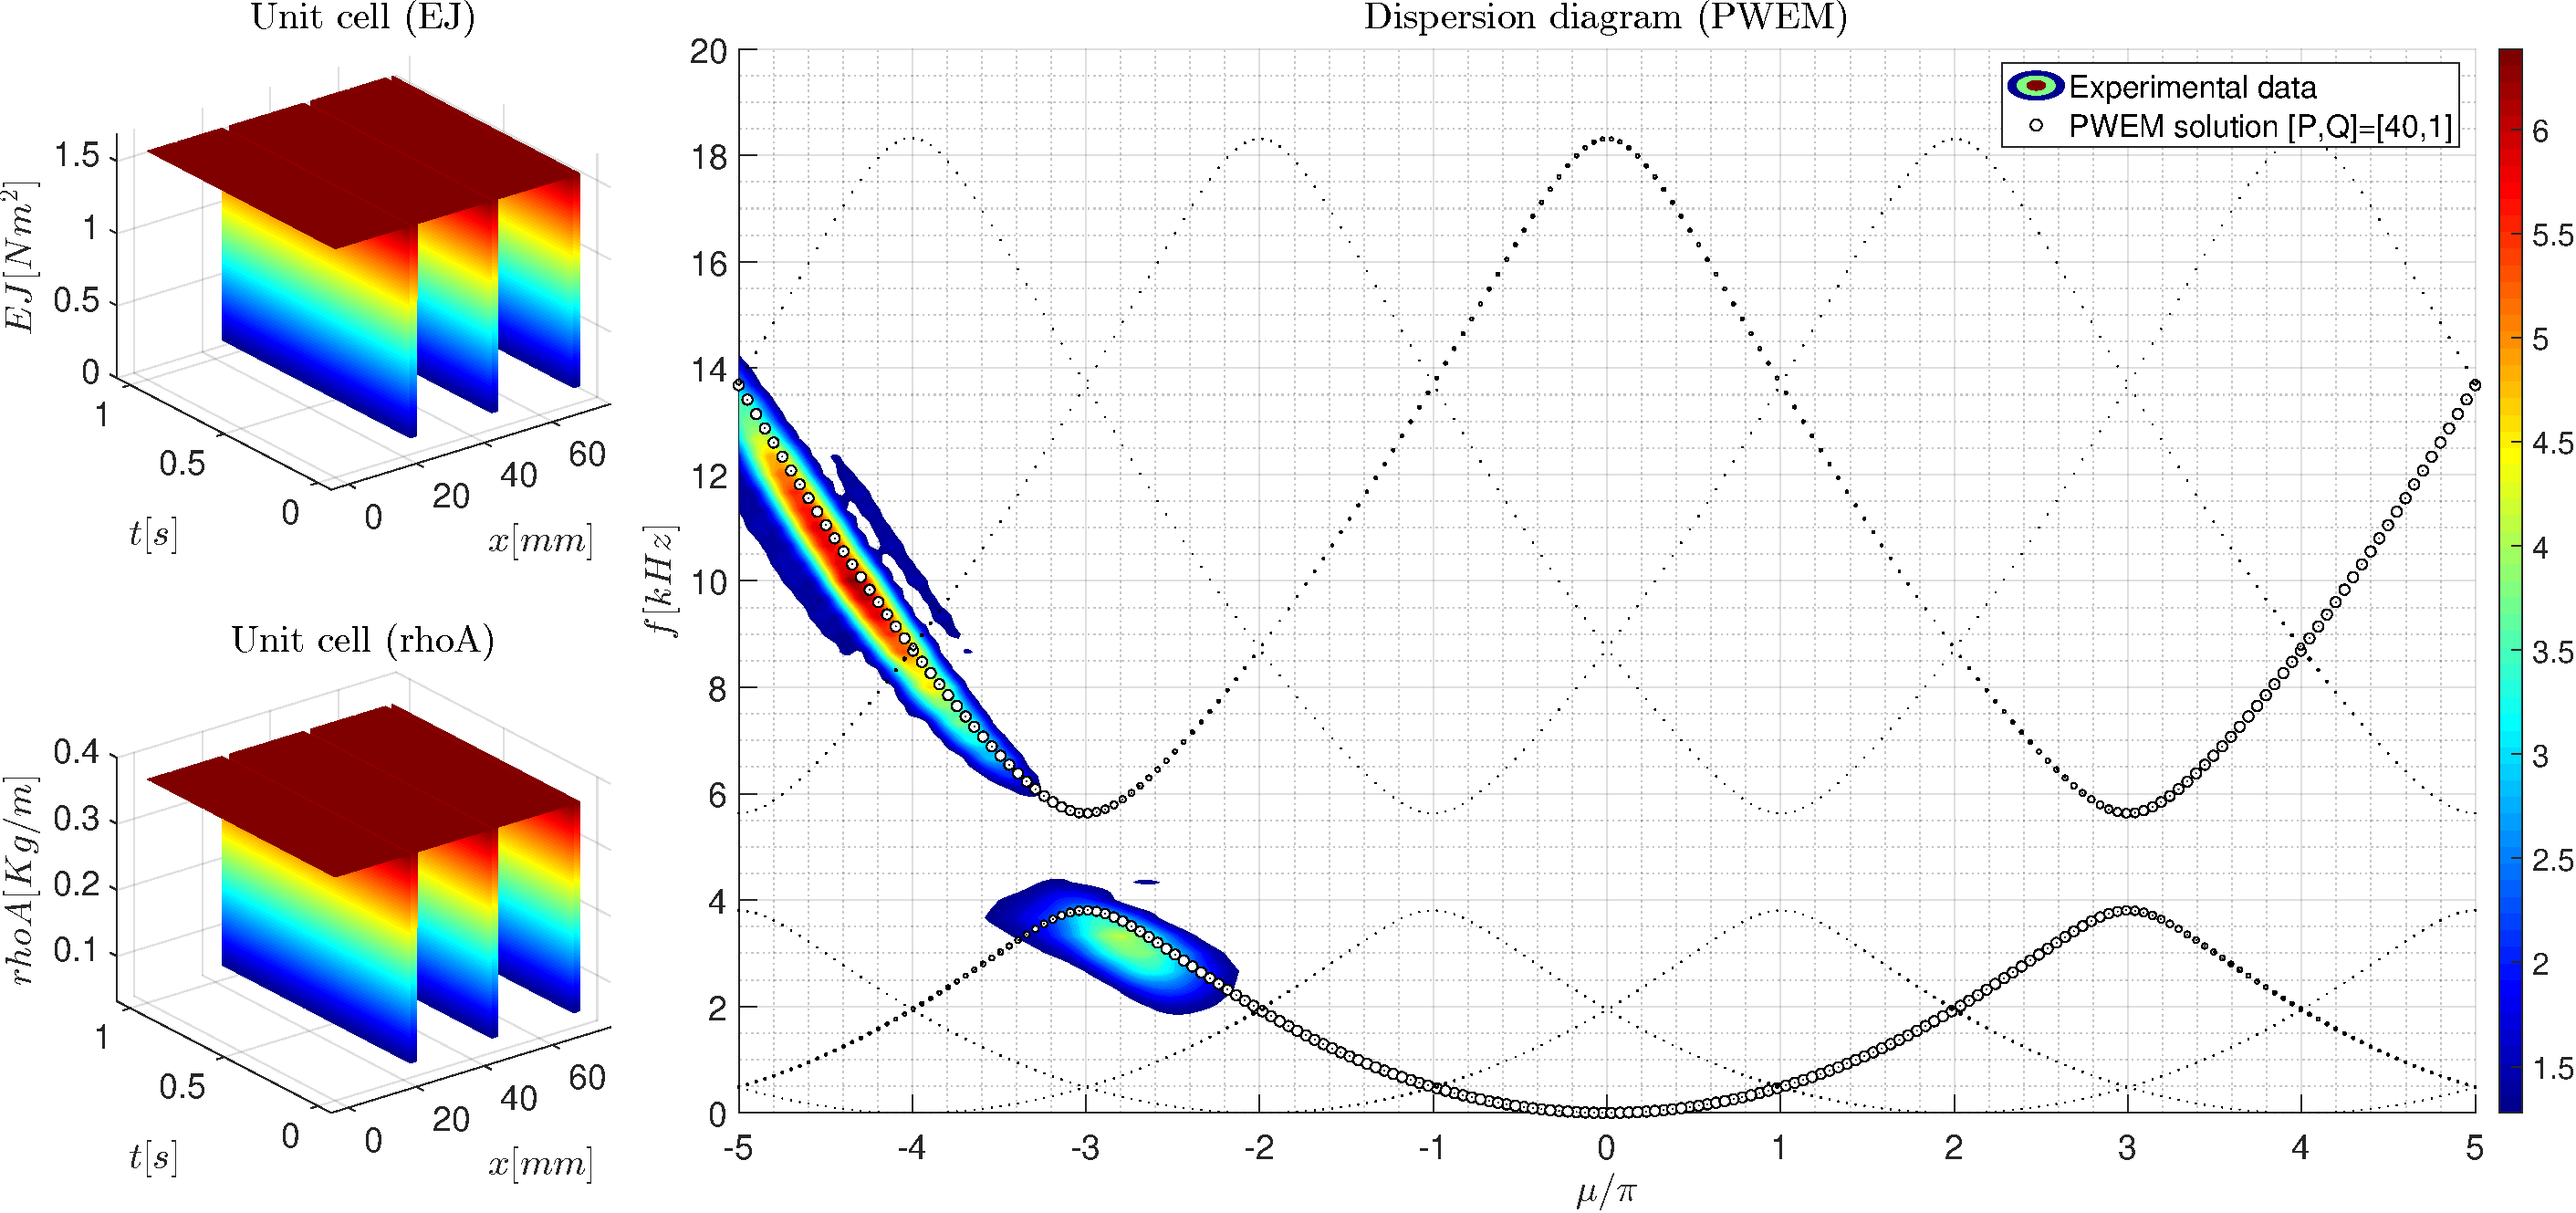
\includegraphics[width=\textwidth]{./img/MATLAB/PWEM_EXP ON-ON-ON @0kHz.pdf}
    \caption{Band structure for the ON-ON-ON configuration.}
    \label{fig:space_only_on_on_on}
\end{figure}

\begin{figure}[H]
    \centering
    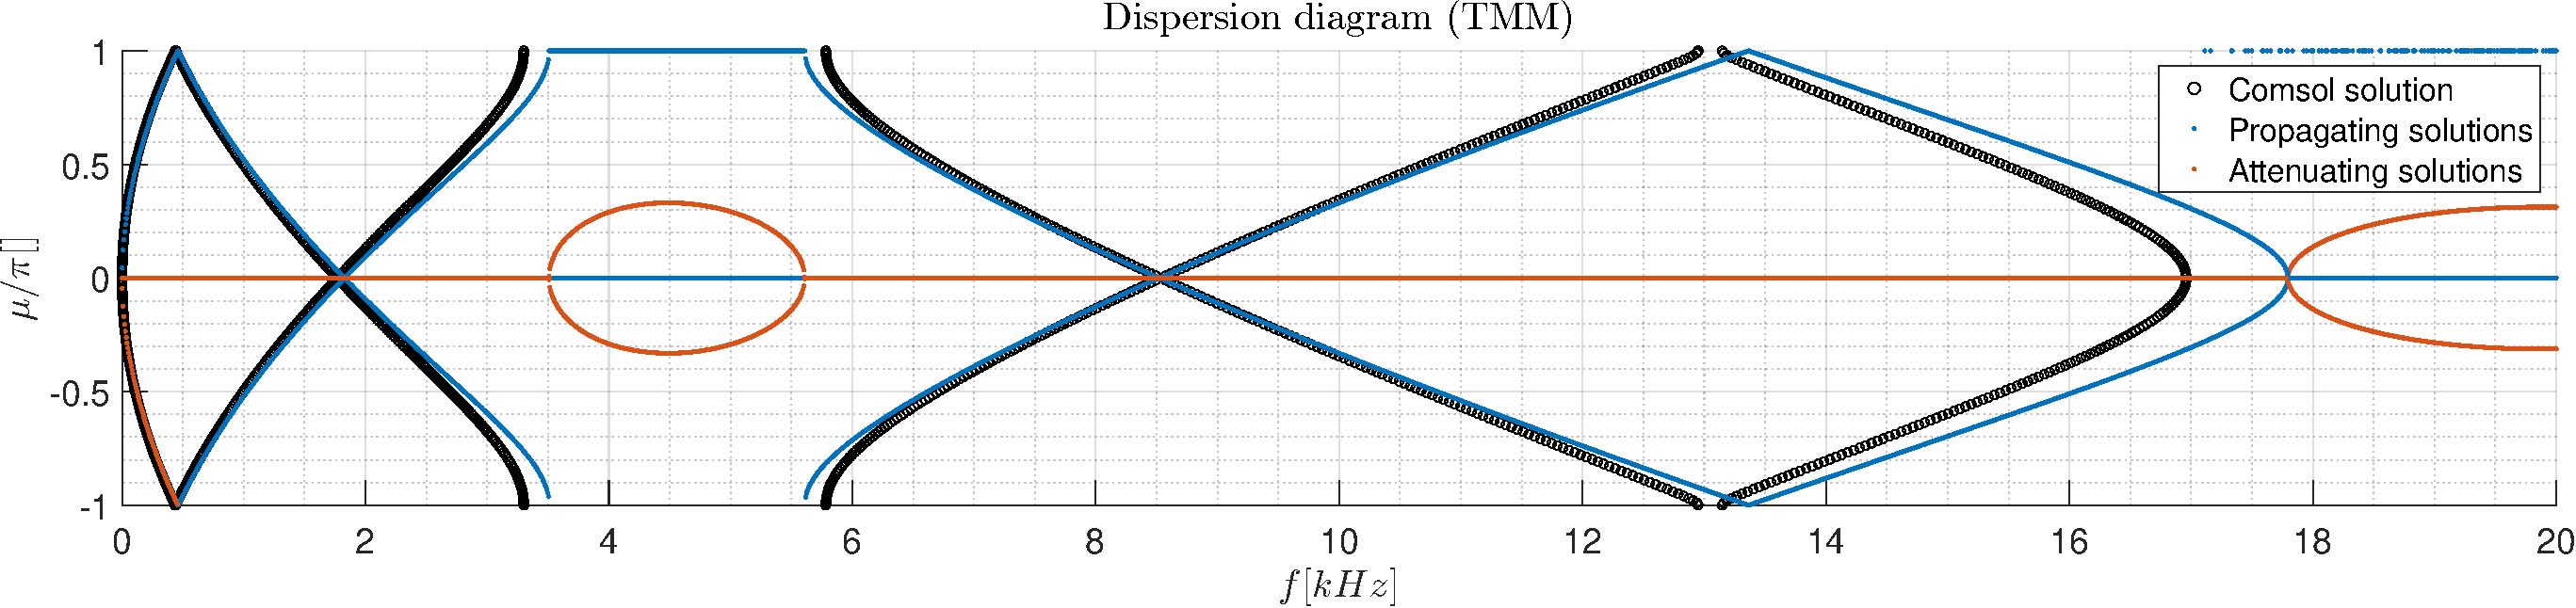
\includegraphics[width=\textwidth]{./img/MATLAB/TMM_COMSOL ON-ON-ON @0kHz.pdf}
    \caption{Comparison between TMM and Comsol Multiphysics for the ON-ON-ON configuration.}
    \label{fig:space_only_on_on_on_comsol}
\end{figure}

Similar consideration as before can be done about the discrepancy between the numerical methods and the experimental data.
Comsol Multiphysics is again used as a reference to validate the experimental results.

With respect to the ON-ON-ON configuration, a shift of the band-gap towards lower frequencies is observed:

\begin{equation}
    f_{BG}^{ON-ON-ON} = [3.4, 5.6] kHz
\end{equation}

This shift is due to the fact that the piezoelectric patches are in the short-circuit state, which results in a lower effective stiffness of the beam section.
Having a lower effective stiffness is equivalent to state that the speed of the travelling wave is lower, which results in a lower frequency of the band-gap.



\paragraph{ON-OFF-OFF}

The last case considered regarding the space-only modulation is the ON-OFF-OFF configuration, where only the first shunt circuit is closed and the other two are open.

It's intuitive to understand that the mechanical admittance is no more the same for the three piezoelectric patches.
This will introduce additional sources of dispersion in the system, which will result in higher number of band-gaps visible in the same frequency range.

Figure \ref{fig:space_only_on_off_off}, shows the PWEM and experimental results, while the comparison between the TMM and Comsol Multiphysics is shown in Figure \ref{fig:space_only_on_off_off_comsol}.

\begin{figure}[H]
    \centering
    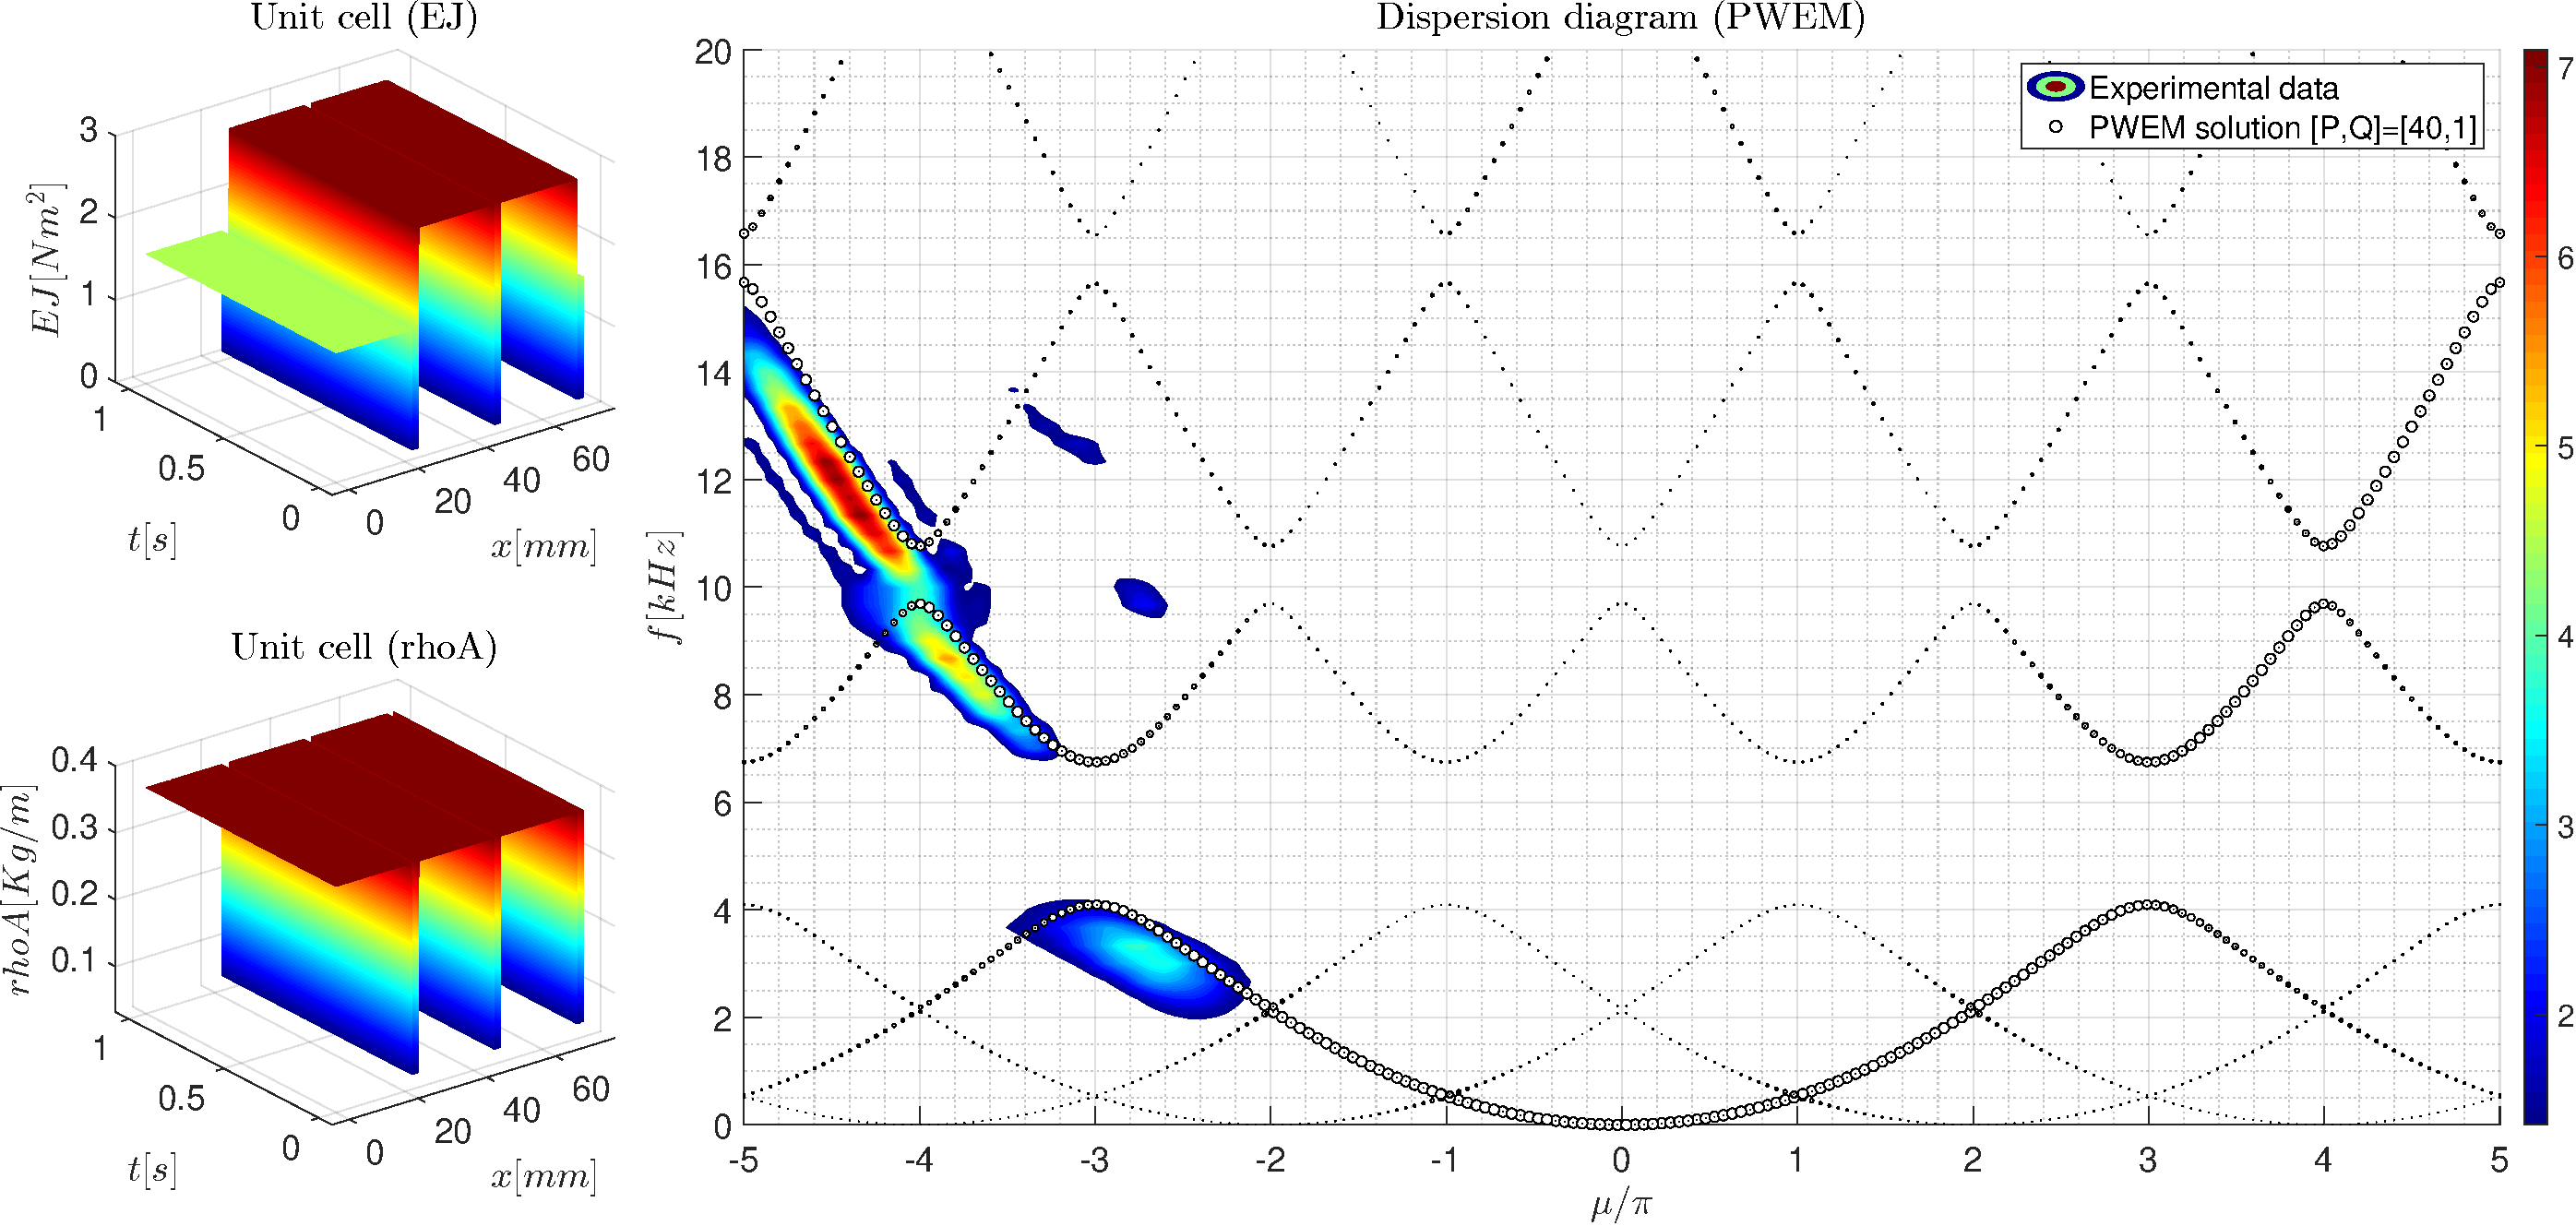
\includegraphics[width=\textwidth]{./img/MATLAB/PWEM_EXP ON-OFF-OFF @0kHz.pdf}
    \caption{Band structure for the ON-OFF-OFF configuration.}
    \label{fig:space_only_on_off_off}
\end{figure}

\begin{figure}[H]
    \centering
    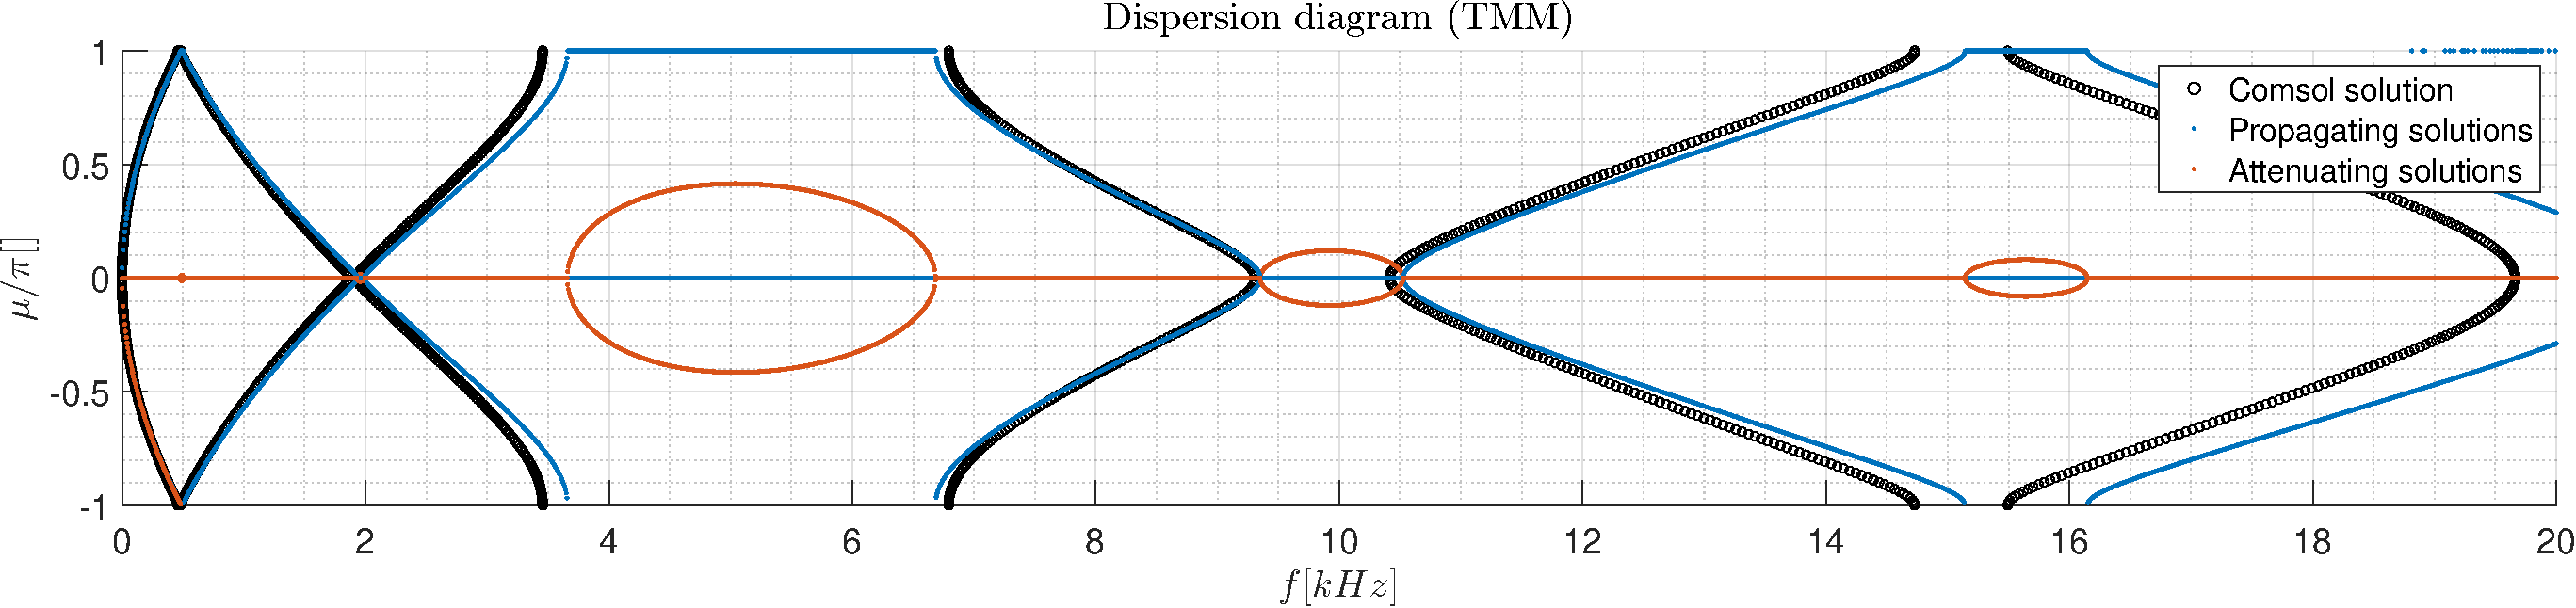
\includegraphics[width=\textwidth]{./img/MATLAB/TMM_COMSOL ON-OFF-OFF @0kHz.pdf}
    \caption{Comparison between TMM and Comsol Multiphysics for the ON-OFF-OFF configuration.}
    \label{fig:space_only_on_off_off_comsol}
\end{figure}

As a confirmation of the previous considerations, the band structure of the ON-OFF-OFF configuration shows a higher number of band-gaps in the same frequency range.

The band gap of the structure are now found at:

\begin{equation}
    \begin{aligned}
        f_{BG1}^{ON-OFF-OFF} & = [3.5, 6.7] kHz   \\
        f_{BG2}^{ON-OFF-OFF} & = [9.3, 10.4] kHz  \\
        f_{BG3}^{ON-OFF-OFF} & = [14.7, 15.5] kHz
    \end{aligned}
\end{equation}

\subsection{Space-Time Modulation}
\label{subsec:space_time_modulation}

For the case of space-time modulations, the three pairs of piezoelectric patches are driven by three equal but shifted in time signals.

The general law guiding the modulation is the following:

\begin{equation}
    Y_k^{SU} = \frac{(Y_1^D + Y_1^E)}{2} + \frac{(Y_1^D - Y_1^E)}{2} sign \left[ \cos \left( 2 \pi f_m t + (k-1) \frac{2\pi}{3} \right) \right]
\end{equation}

Where $Y_k^{SU}$ is the mechanical admittance of the $k$-th piezoelectric patch in the spatiotemporal (ST) cell, $Y_1^D$ and $Y_1^E$ are the mechanical admittance of the piezopatch in case of open and short circuit, respectively, and $f_m$ is the modulation frequency.

The phase shift between piezelectric patches imposed by the modulation $\phi=\frac{\pi}{3}$, is necessary to achieve directionality in the structure.
Thanks to this phase shift, and by properly choosing the sign of the modulation frequency, it's possible to to study both the forward and backward directionality of the wave withouth changing the excitation frequency nor it's application point.

In the following, the results of three different pairs ($\pm$) modulation frequencies are presented, and the nonreciprocal behavior of the structure is highlighted.
As for the space modulation, the experimental data are compared with the theoretical predictions obtained through the PWEM method.


\paragraph{Modulation $f_m = \pm 1 kHz$}

Forcing time modulation besides space modulation, causes dispersion diagram to becomes anti-symmetric and some of the band-gaps to be no longer global, but being localized and confined to a specific range of wavenumbers.
This is a clear indication of the nonreciprocal behavior of the structure, for which a more detailed analysis is provided in Section \ref{sec:nonreciprocal_behavior}.

Figure \ref{fig:PWEM_EXP_Sinusoidal_(discrete)_@1kHz} shows the dispersion diagram for the case of modulation frequency $f_m = \pm 1 kHz$.

\begin{figure}[H]
    \centering
    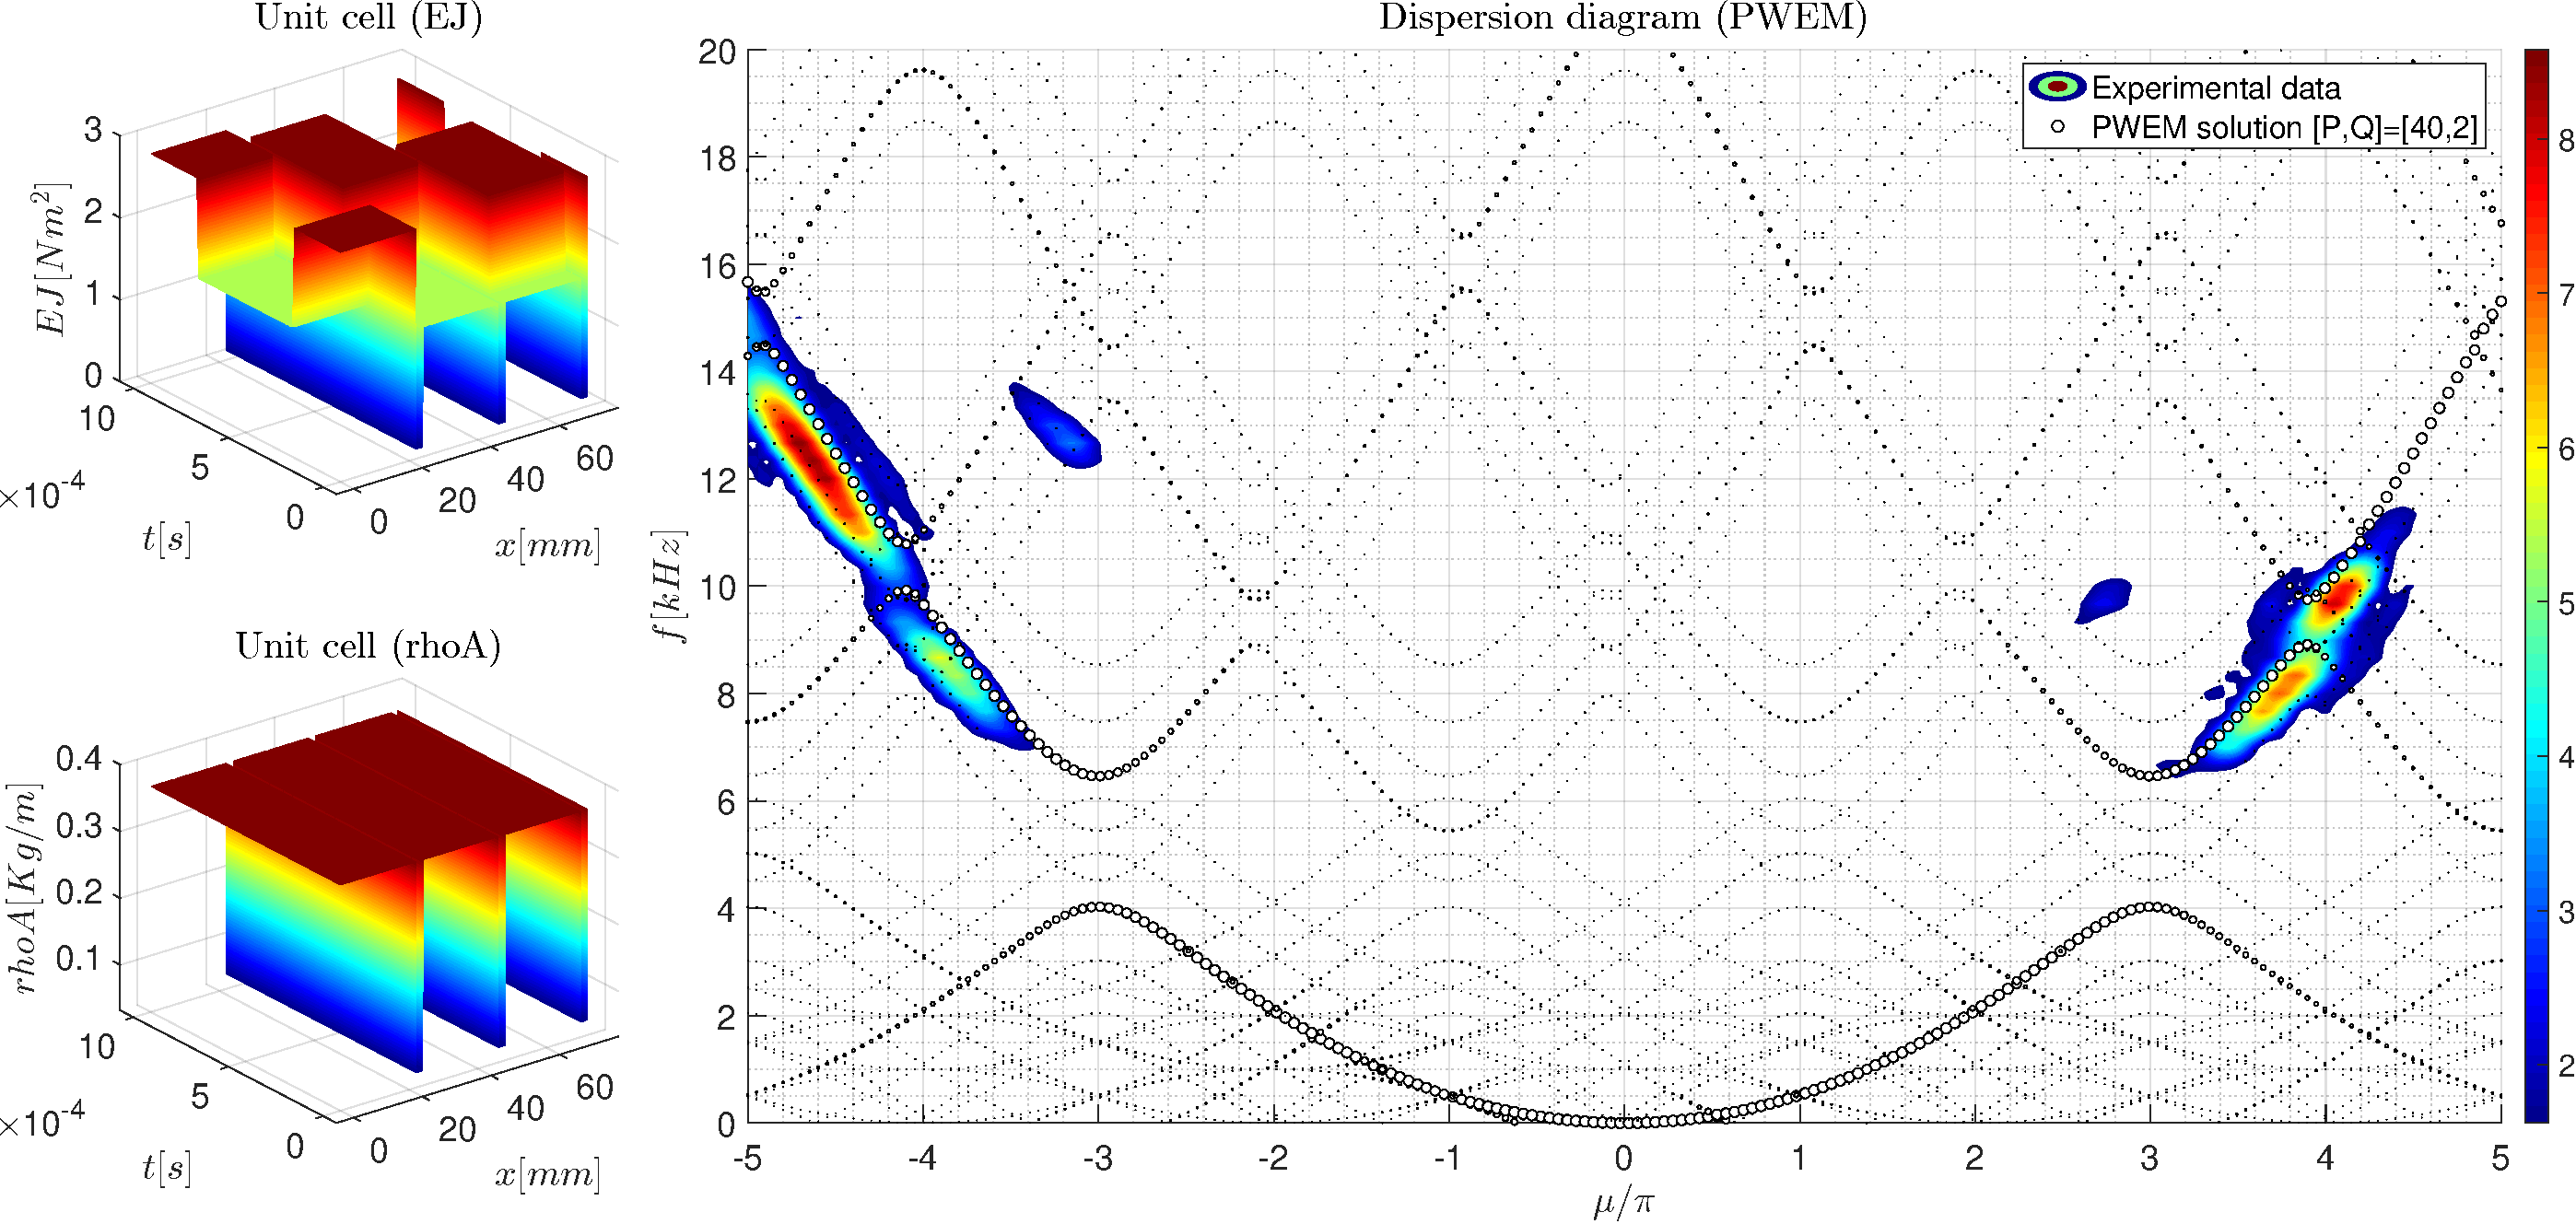
\includegraphics[width=\textwidth]{img/MATLAB/PWEM_EXP Sinusoidal (discrete) @1kHz.pdf}
    \caption{Dispersion diagram for the case of modulation frequency $f_m = \pm 1 kHz$.}
    \label{fig:PWEM_EXP_Sinusoidal_(discrete)_@1kHz}
\end{figure}

Similarly to the case of space modulation, the dispersion diagram coming from the PWEM is compared with the experimental data.
Again, except for the slight discrepancy given by the low number of harmonics considered in the PWEM, the agreement is sufficient to validate the model.

Analyzing the dispersion diagram, it's possible to observe how the first band-gap is associated with spatial modulation, while at higher frequencies nonreciprocal band-gaps associated with the time modulation appear.
In particular, it's possible to observe that at around $8.5kHz$, the first directional band-gap appears.
For the frequency range $8.5kHz < f < 9.5kHz$, we observe a band-gap for positive wavenumbers, being instead transparent in the negative wavenumber range.
On the other hand, for the frequency range $9.5kHz < f < 10.5kHz$, the band-gap is transparent for positive wavenumbers and opaque for negative wavenumbers.



\paragraph{Modulation $f_m = \pm 2 kHz$}

Similar considerations as before can be made for the case of modulation frequency $f_m = \pm 2 kHz$.

Figure \ref{fig:PWEM_EXP_Sinusoidal_(discrete)_@2kHz} shows the dispersion diagram for the case of modulation frequency $f_m = \pm 2 kHz$.

\begin{figure}[H]
    \centering
    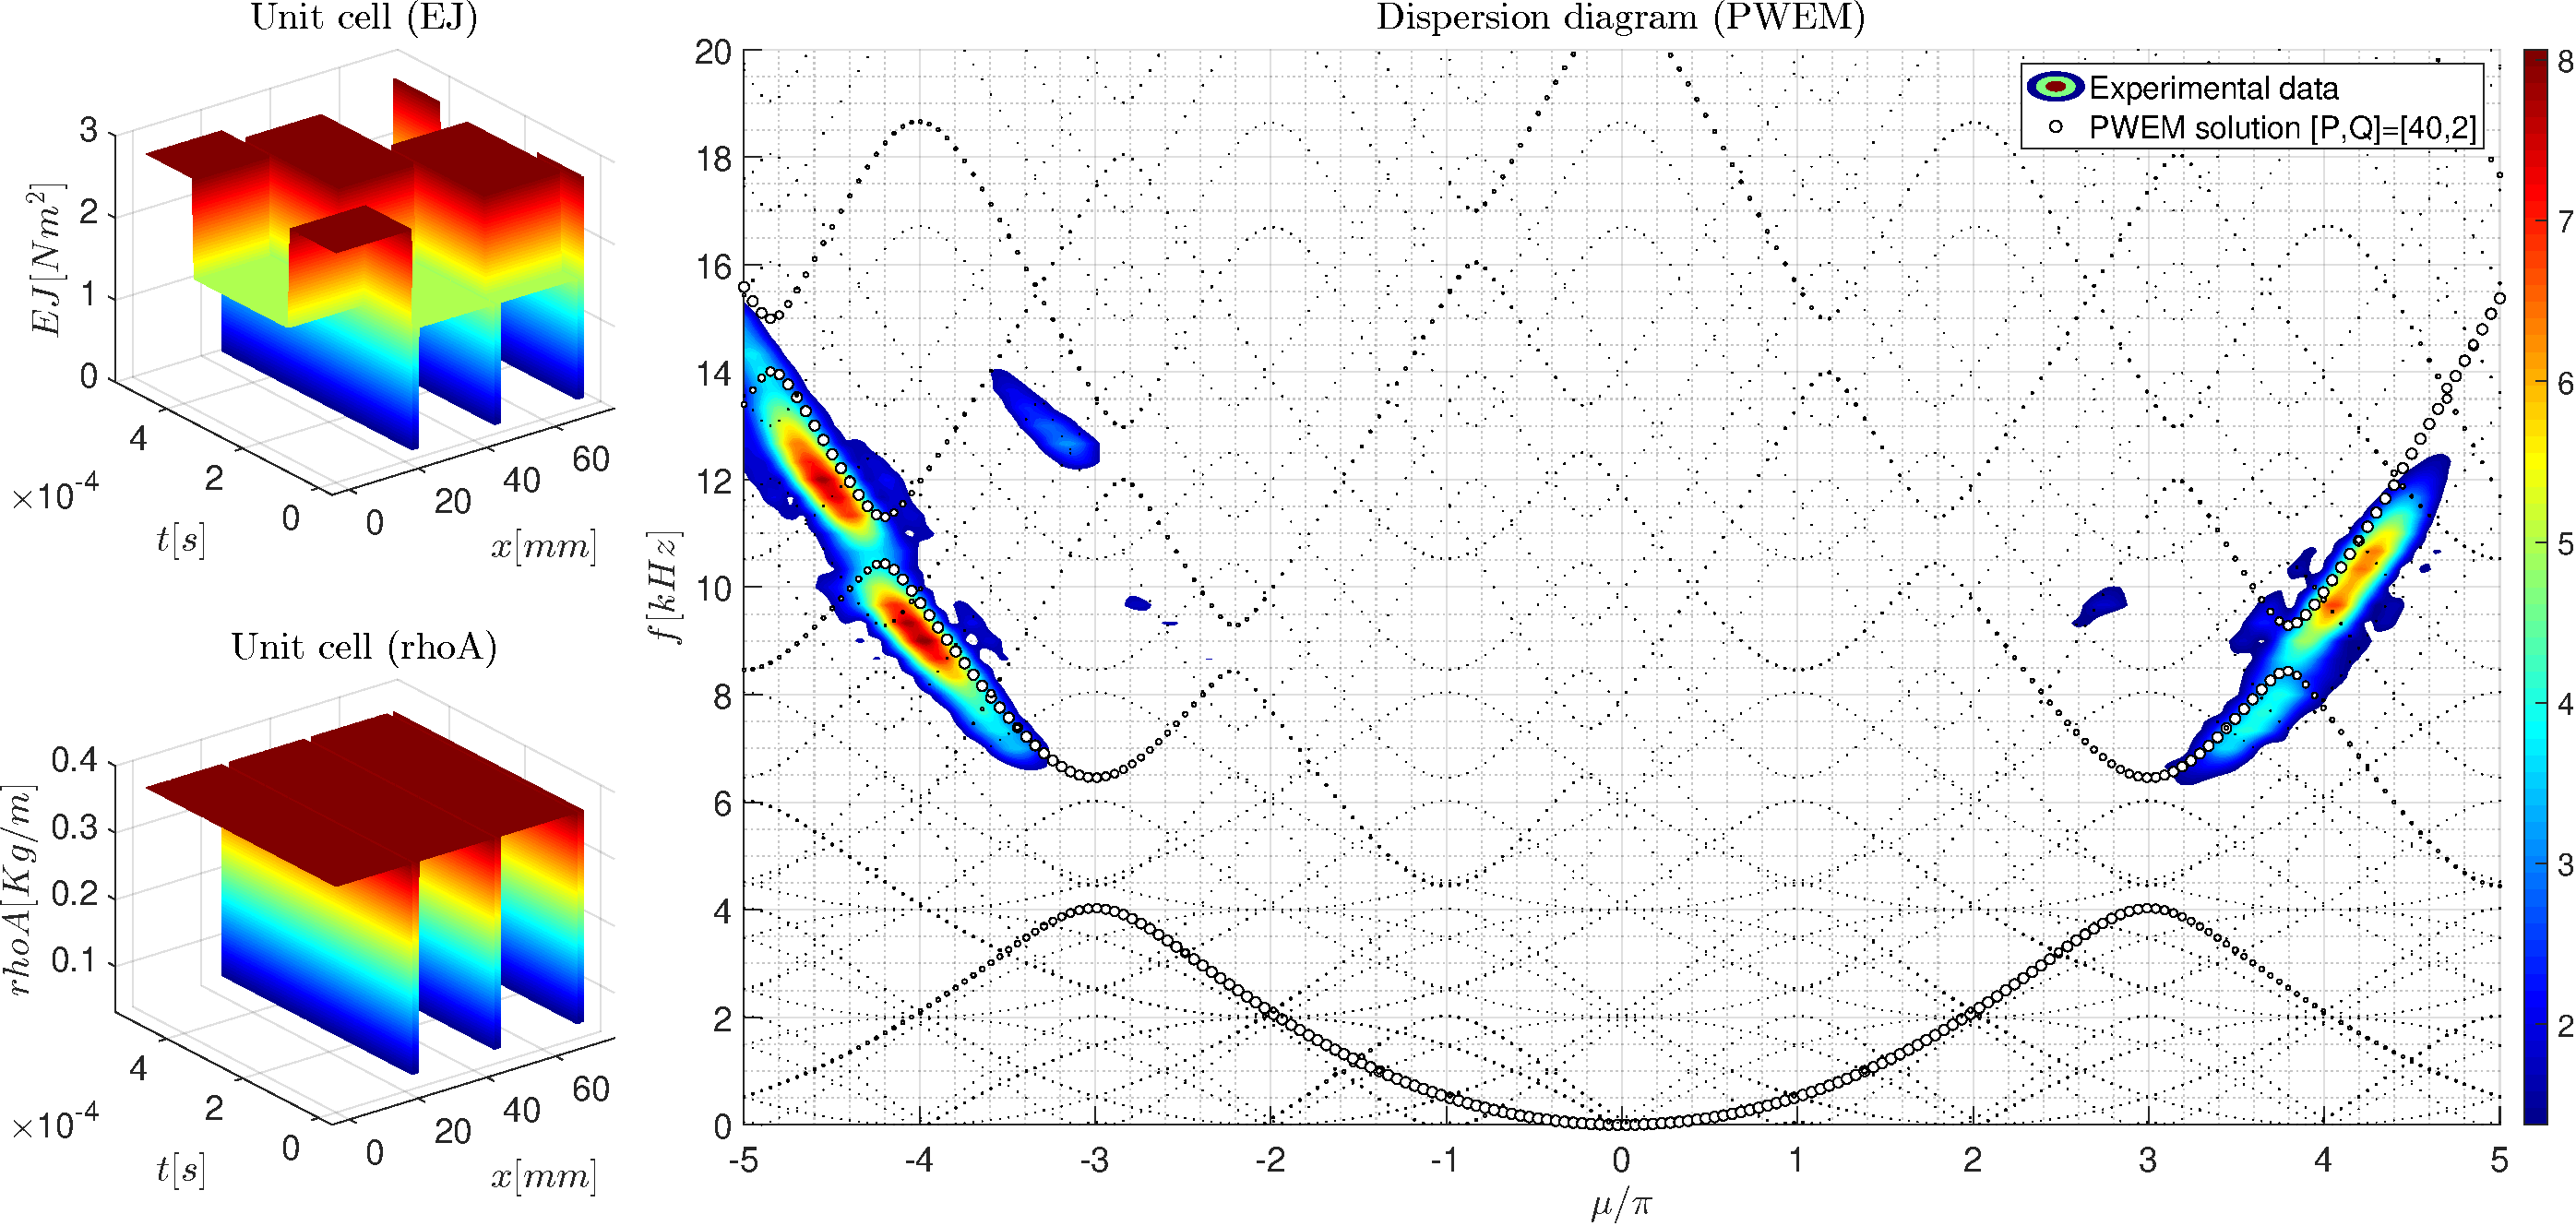
\includegraphics[width=\textwidth]{img/MATLAB/PWEM_EXP Sinusoidal (discrete) @2kHz.pdf}
    \caption{Dispersion diagram for the case of modulation frequency $f_m = \pm 2 kHz$.}
    \label{fig:PWEM_EXP_Sinusoidal_(discrete)_@2kHz}
\end{figure}

Similarly to the previous case, the dispersion diagram coming from the PWEM is compared with the experimental data.

Intuitively, the phenomenon associated with the nonreciprocal behavior is now more pronounced, as the modulation frequency is doubled.
The asymmetrical shift of the already previously analyzed directional band-gaps is even more evident.
A positive and negative shift of almost $0.5kHz$ are observed for the negative and positive wavenumbers bang-gaps, respectively.

Notice that the global band-gap at lower frequencies ($4 < f < 6.5 kHz$) is still present and hasn't been affected by the time modulation.
It's now clear that this band-gap is associated with the spatial modulation only.



\paragraph{Modulation $f_m = \pm 3 kHz$}

Figure \ref{fig:PWEM_EXP_Sinusoidal_(discrete)_@3kHz} shows the dispersion diagram for the case of modulation frequency $f_m = \pm 3 kHz$.

\begin{figure}[H]
    \centering
    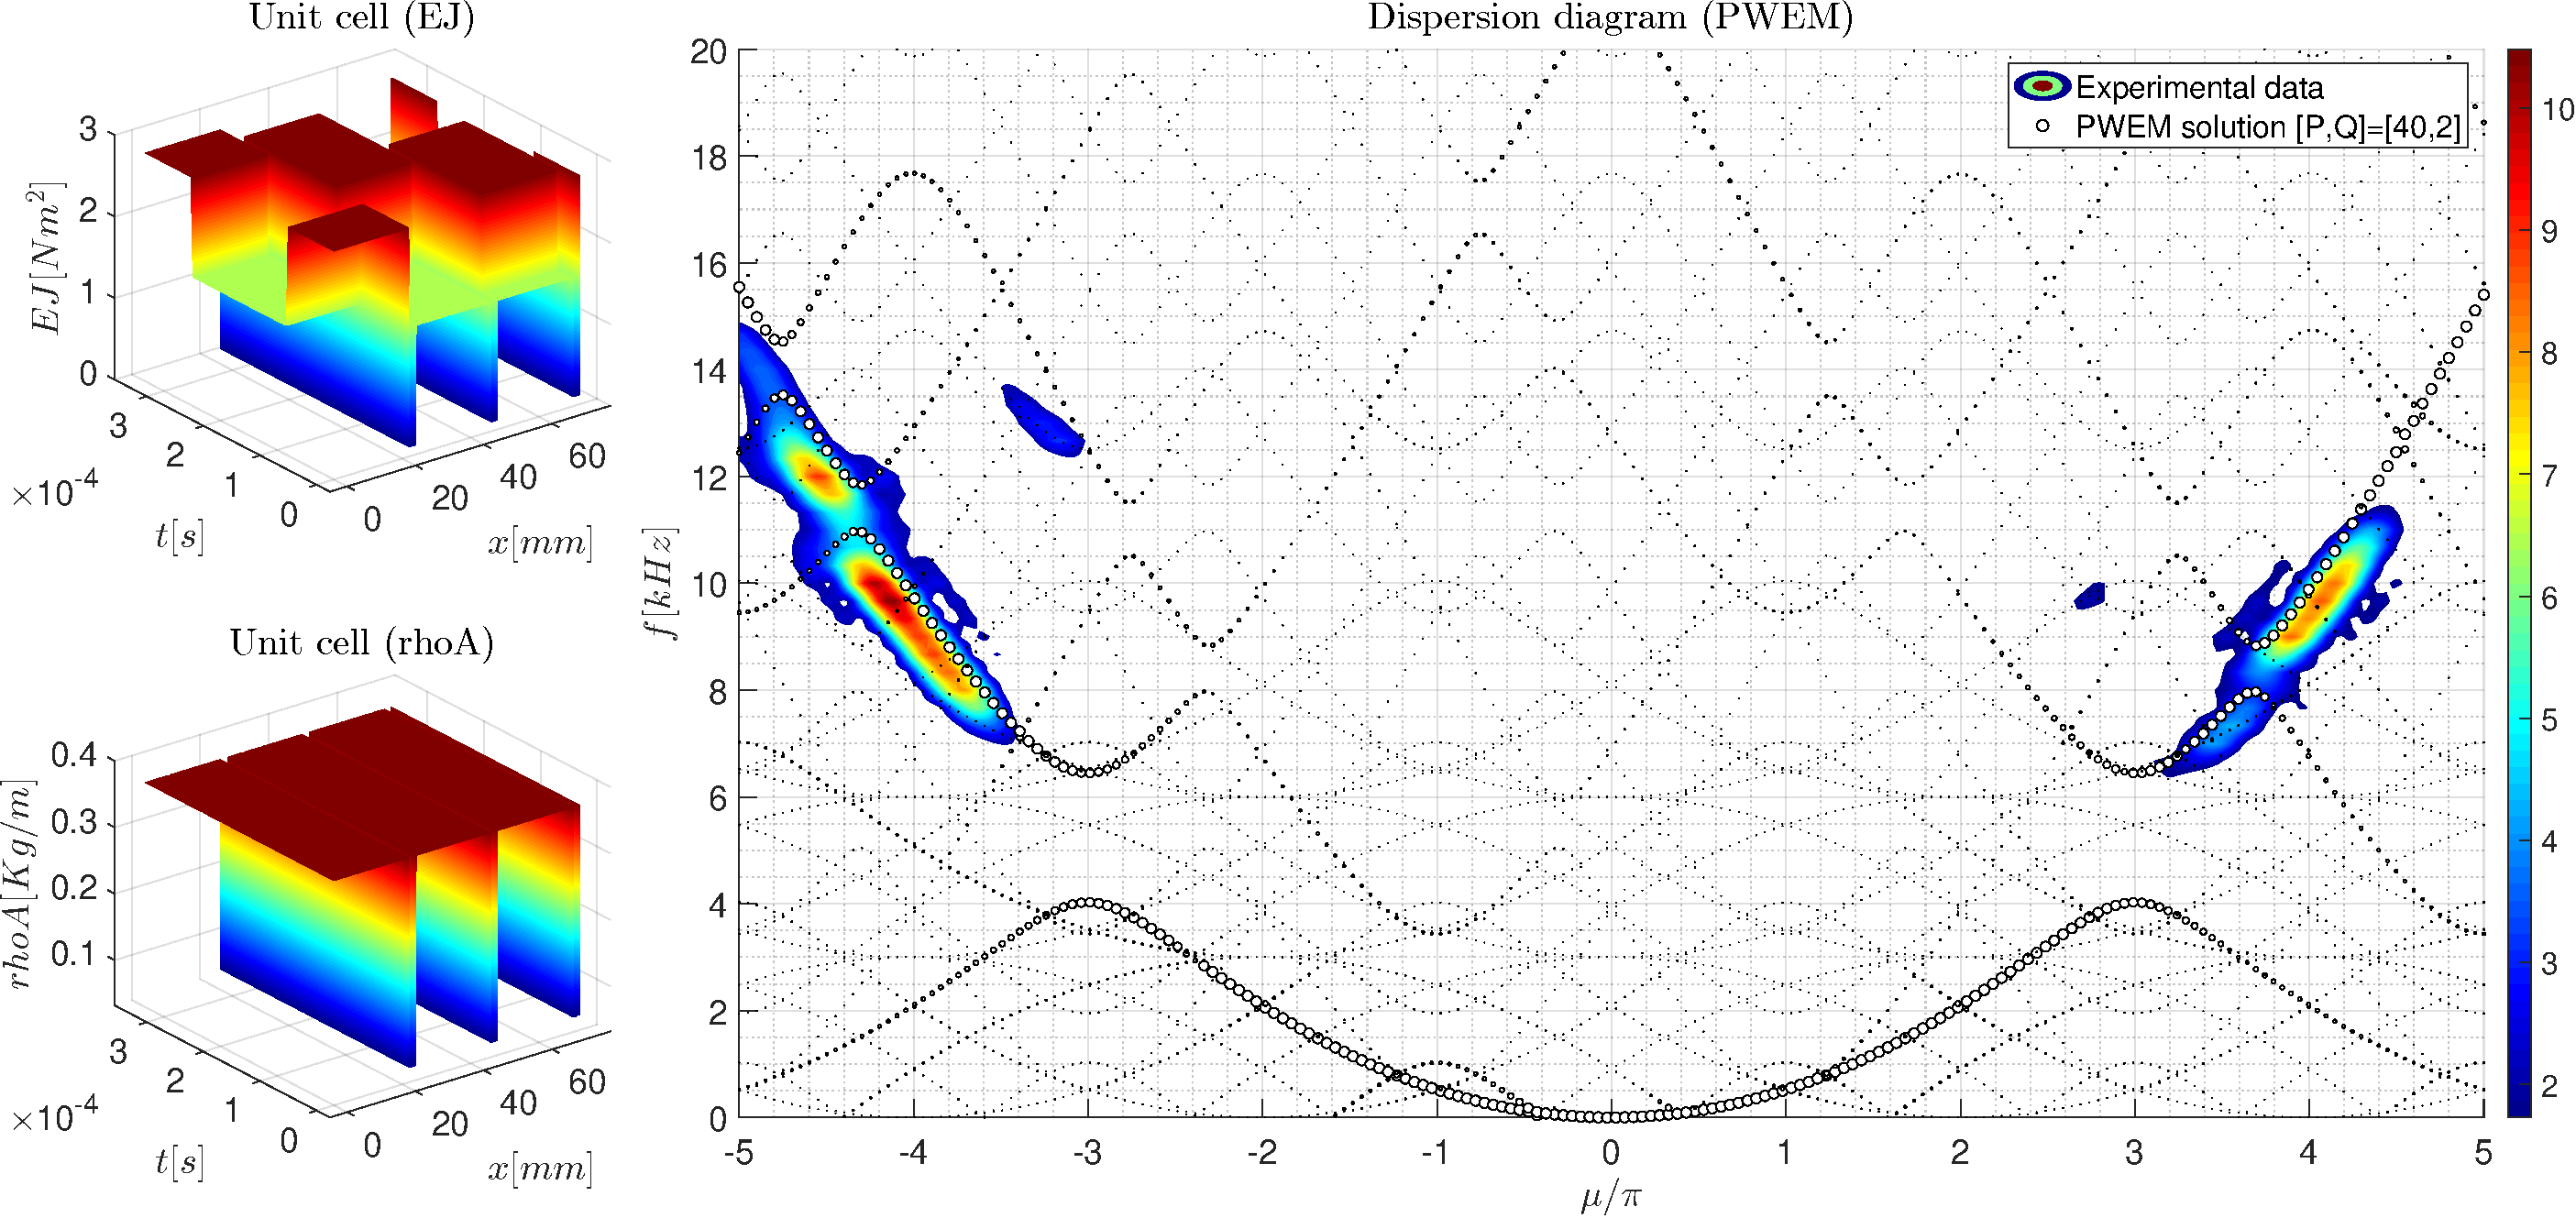
\includegraphics[width=\textwidth]{img/MATLAB/PWEM_EXP Sinusoidal (discrete) @3kHz.pdf}
    \caption{Dispersion diagram for the case of modulation frequency $f_m = \pm 3 kHz$.}
    \label{fig:PWEM_EXP_Sinusoidal_(discrete)_@3kHz}
\end{figure}

Same considerations as before can be made for the case of modulation frequency $f_m = \pm 3 kHz$.
As the modulation frequency increases, also the nonreciprocal behavior becomes more pronounced.




\section{Nonreciprocal behavior}
\label{sec:nonreciprocal_behavior}

From the experimental results of the previous section, an important aspect has been highlighted related to the nonreciprocal behavior of the structure when excited with a time-space modulated signal.
In this section we aim at further investigate this aspect by performing additional experimental tests on the structure.



\subsection{Tests description}
\label{subsec:nonreciprocal_behavior_setup}

Using the same geometry and setup as in the previous sections (see Section \ref{subsec:experimental_setup}), we aim at exciting the structure at the two directional band-gaps frequencies observed in the previous section when modulating the shunts at $f_m = \pm 2 kHz$ are be analyzed.

For convenience, we report in Figure \ref{fig:nonreciprocal_behavior_2kHz} a zoomed-in version of the dispersion diagram around the two directional band-gaps frequencies $f_{BG}^- = [10 11] kHz$ and $f_{BG}^+ = [8 9] kHz$.

\begin{figure}[H]
    \centering
    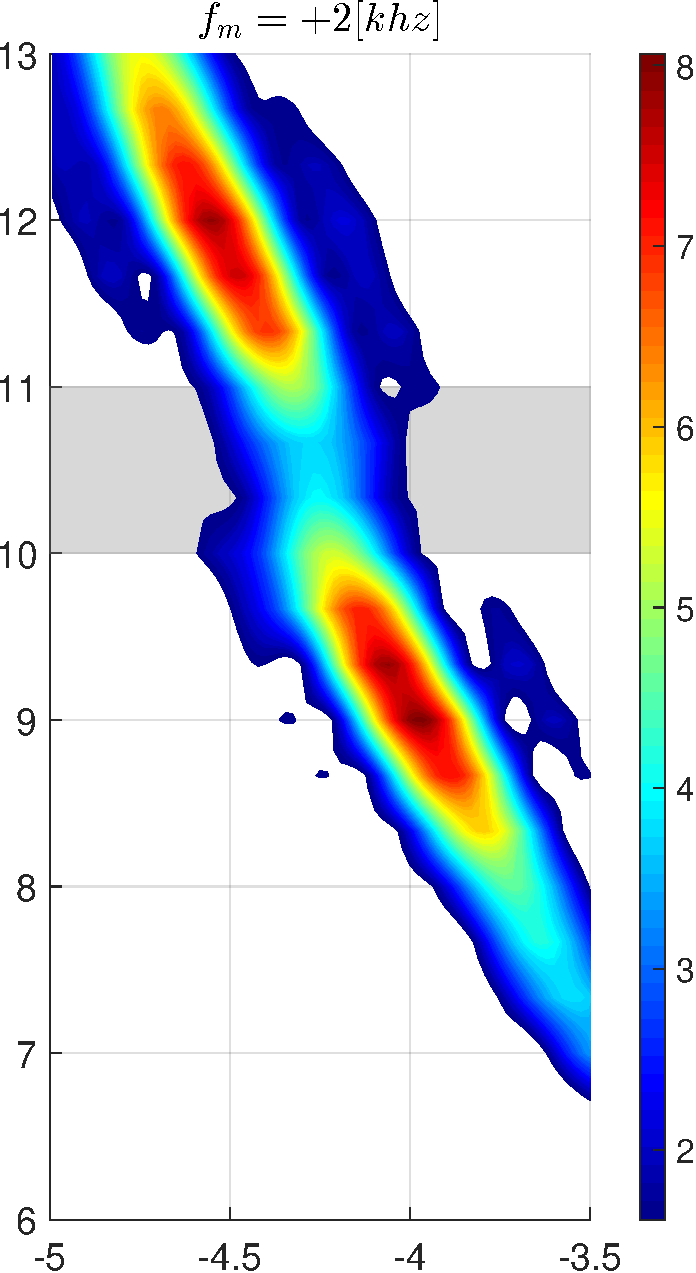
\includegraphics[width=0.3\textwidth]{img/MATLAB/EXP_nonreciprocal_@+2kHz.pdf}
    \hspace{2cm}
    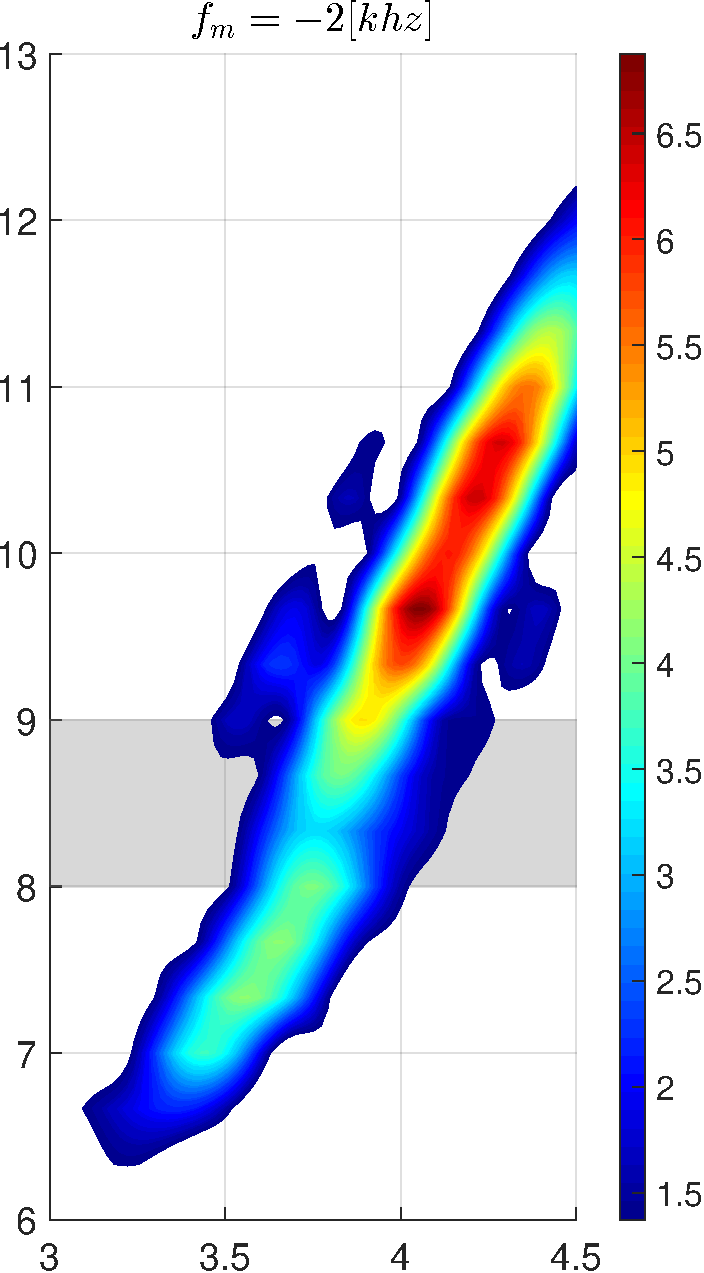
\includegraphics[width=0.3\textwidth]{img/MATLAB/EXP_nonreciprocal_@-2kHz.pdf}
    \caption{Dispersion diagram for the case of modulation frequency $f_m = \pm 2 kHz$.}
    \label{fig:nonreciprocal_behavior_2kHz}
\end{figure}

Two tests are now performed.

At first, a tone-burst excitation signal with central frequency $f_e = 8.4 kHz$ and delta frequency $\Delta f = 0.4 kHz$ is applied while modulating the shunts in one case at $f_m = +2 kHz$ and in the other case at $f_m = -2 kHz$.

Secondly, in a similar fashion, the higher frequency directional band-gaps is excited with a tone-burst signal having central frequency $f_e = 10.5 kHz$ and $\Delta f = 0.5 kHz$.
The shunts are modulated at the same frequencies as before ($f_m = \pm 2 kHz$).

The excitation signal is still applied as before at the same point along the beam, but the change in the sign of modulation frequency of the shunts has the same effect as changing the direction of the wave propagation.
Thanks to this property, the experimental setup remains unchanged while still allowing to investigate the nonreciprocal behavior of the structure.



\subsection{Results}
\label{subsec:nonreciprocal_behavior_results}

The obtained experimental data align with what has already been in present in Section \ref{subsec:space_time_modulation}: because of time-modualtion of the shunts and so of the piezoelectric patches, the structure responds differently to the same excitation signal depending on the direction of the travelling wave.

This aspect is visible also from the waterfall plots of the beam displacement.
The diagrams below shows the trasversal displacement of some points along the beam as a function of time.
Depeneding on the excitation signal and the modulation frequency, the displacement at the end of the beam is different in the two cases.

\paragraph{Lower directional band-gaps $f_{BG}^+ = [8, 9] kHz$}

The waterfall plots in Figure \ref{fig:nonreciprocal_behavior_8p4kHz} show the trasversal beam displacement for the case of excitation at $f_e = 8.4 kHz$ and modulation at $f_m = \pm 2 kHz$.

\begin{figure}[H]
    \centering
    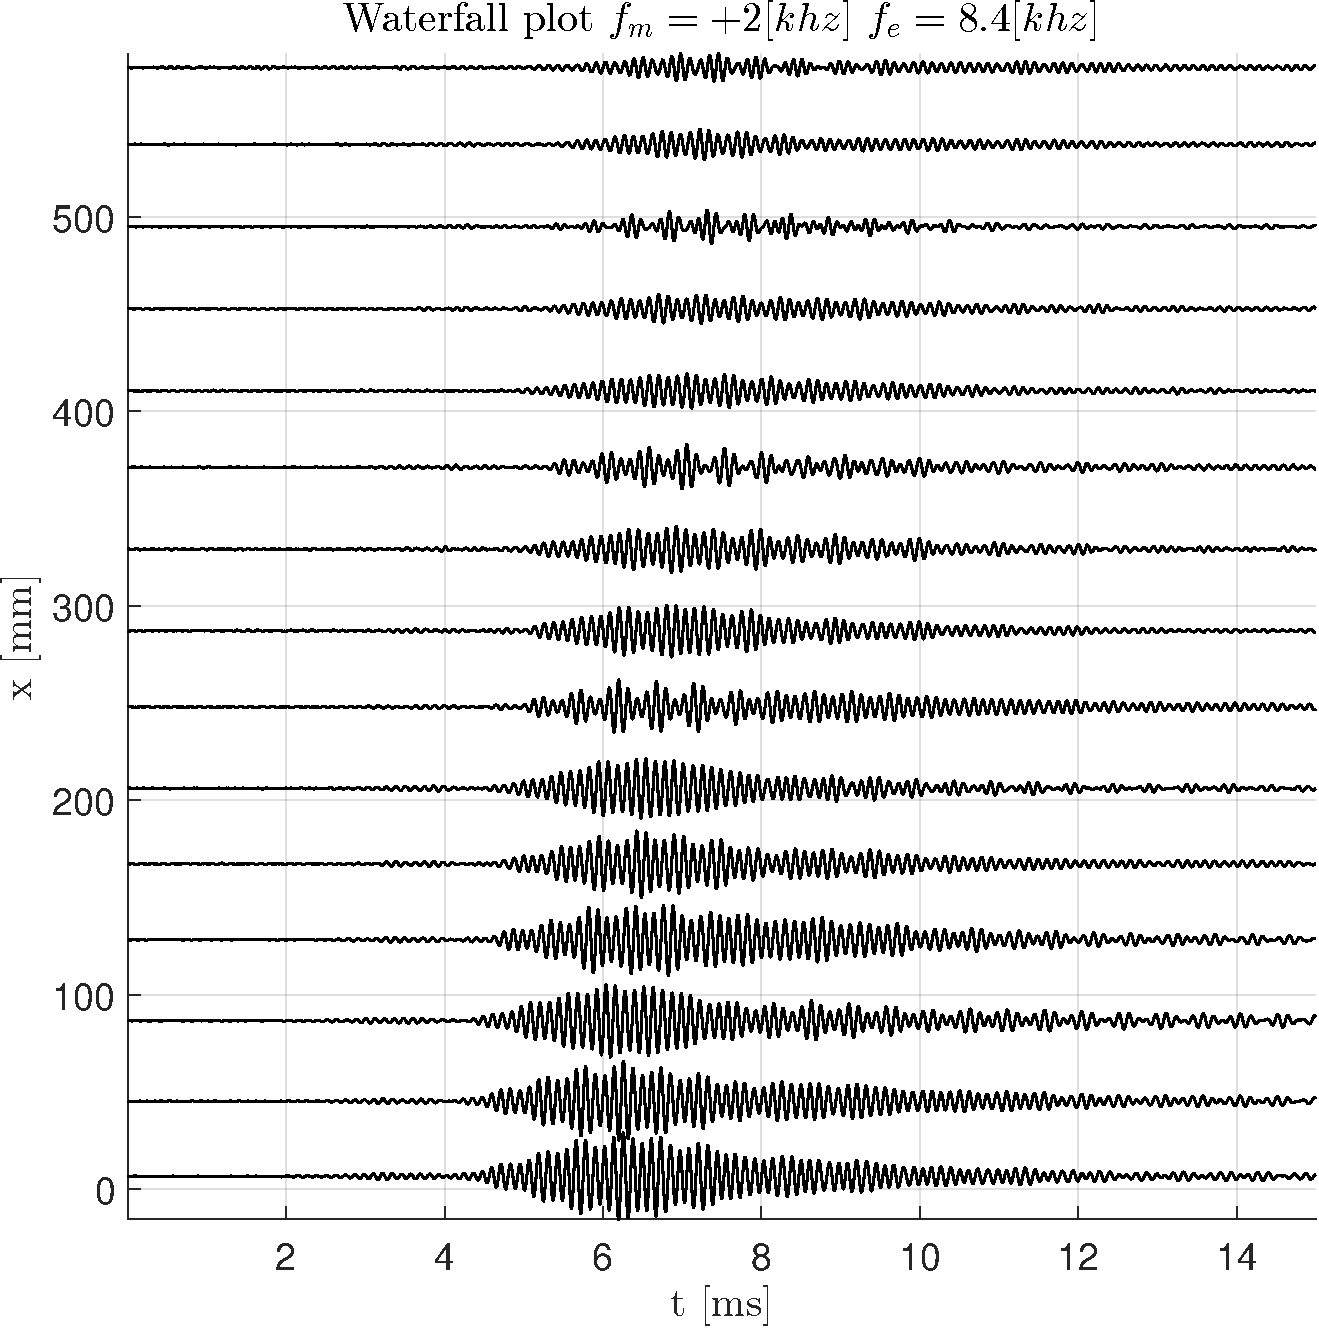
\includegraphics[width=0.45\textwidth]{img/MATLAB/EXP_Scan_time_narrow8p4kHz_2000plus.unv.pdf}
    \hspace{1cm}
    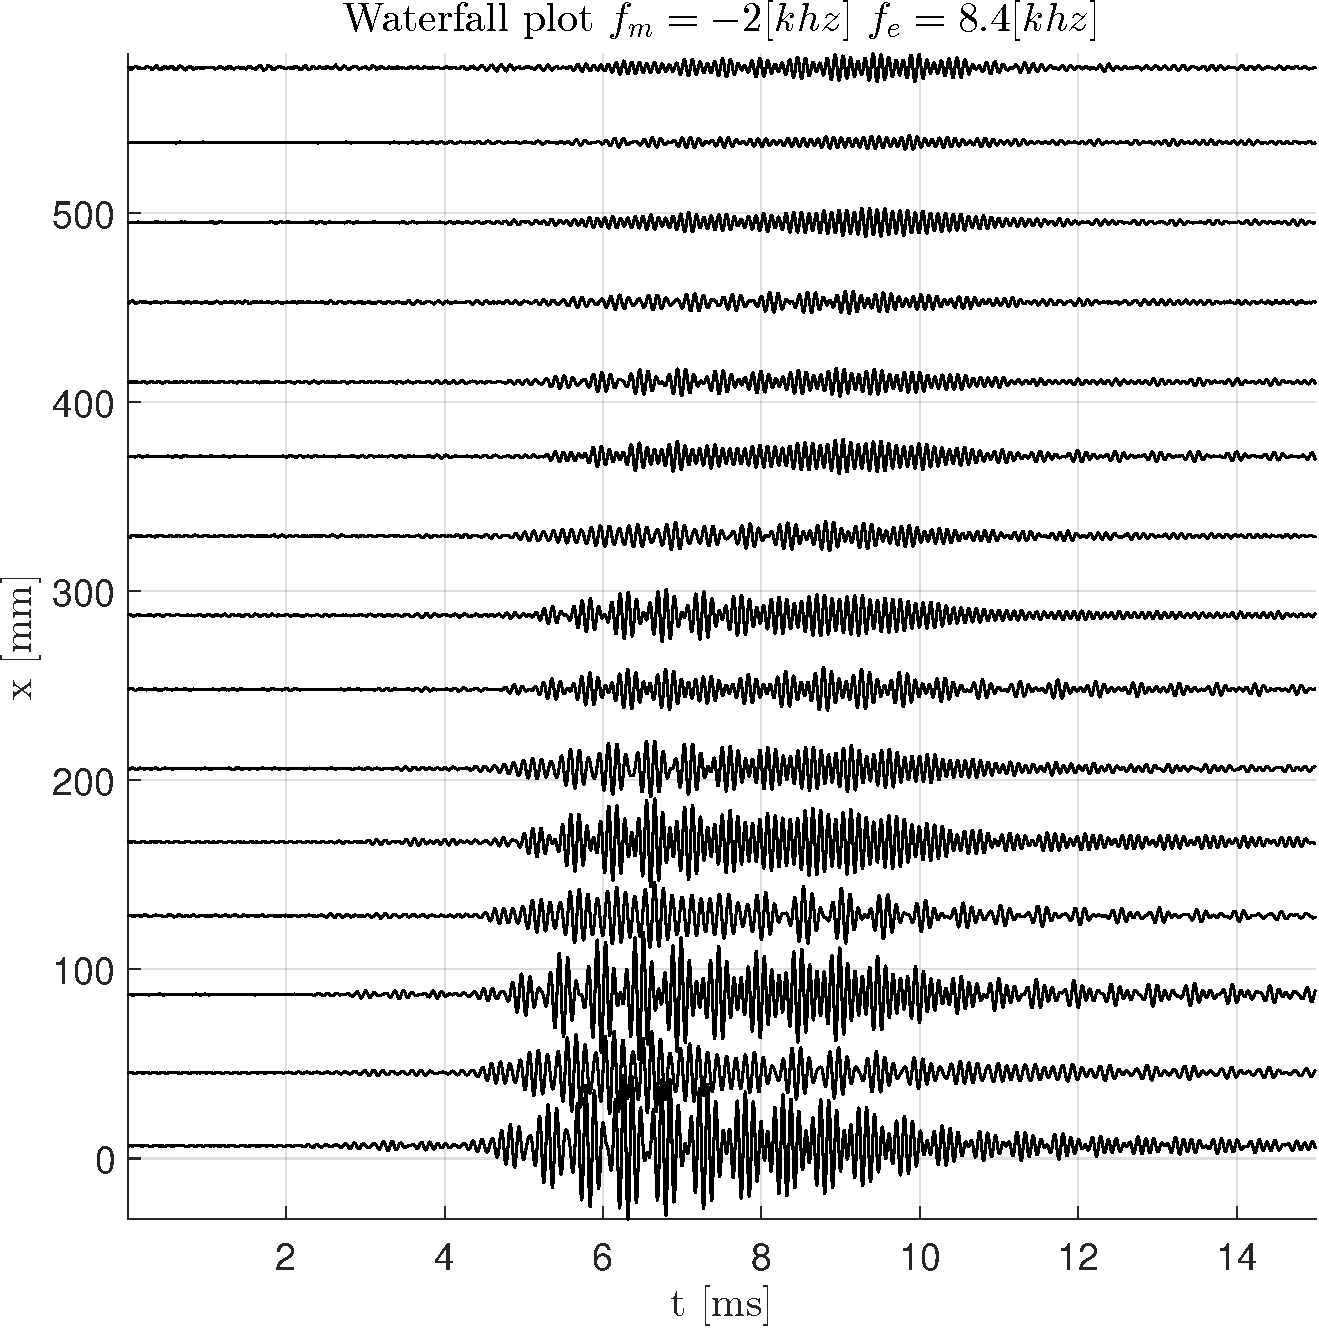
\includegraphics[width=0.45\textwidth]{img/MATLAB/EXP_Scan_time_narrow8p4kHz_2000minus.unv.pdf}
    \caption{Waterfall plot of the beam displacement for the case excitation at $f_e = 8.4 kHz$ and modulation at $f_m = +2 kHz$ (left) and $f_m = -2 kHz$ (right).}
    \label{fig:nonreciprocal_behavior_8p4kHz}
\end{figure}

Even if not clearly visible from the waterfall plots, the attenuation of the wave is different depending on the propagation direction.
Referring to Figure \ref{fig:nonreciprocal_behavior_2kHz}, we expected to obtain a stronger attenuation for the case of negative modulation frequency and, instead, a weaker attenuation for the case of positive modulation frequency.

Even if waterfall plots in this case do not show a clear difference in the attenuation of the wave, we can plot the spectra of the displacement signals at the end of the beam in the two cases to better observe the behavior of the structure.
The spectra are shown in Figure \ref{fig:nonreciprocal_behavior_8p4kHz_spectra}.

\begin{figure}[H]
    \centering
    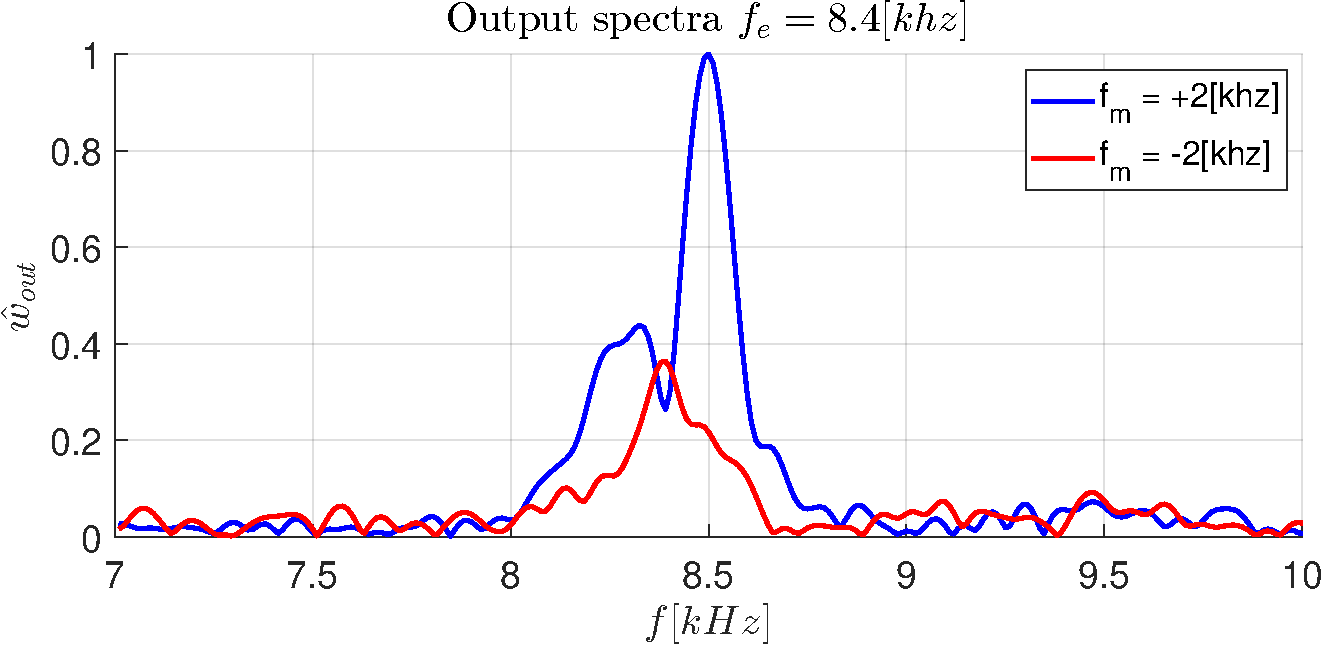
\includegraphics[width=0.7\textwidth]{img/MATLAB/Spectra_narrow8p4kHz_2000.pdf}
    \caption{Normalized spectra of the beam displacement at the end of the beam for the case of excitation at $f_e = 8.4 kHz$ and modulation at $f_m = \pm 2 kHz$.}
    \label{fig:nonreciprocal_behavior_8p4kHz_spectra}
\end{figure}

The spectra show that the attenuation of the wave is indeed different in the two cases.
The attenuation is in fact stronger in the case of negative modulation frequency, given that we find the directional band-gap at $f_{BG}^+ = [8, 9] kHz$.
On the other hand, the attenuation is weaker in the case of positive modulation frequency, given that no band-gap is present.


\paragraph{Higher directional band-gaps $f_{BG}^- = [10, 11] kHz$}

The waterfall plots in Figure \ref{fig:nonreciprocal_behavior_10p5kHz} show the beam displacement for the case of excitation at $f_e = 10.5 kHz$ and modulation at $f_m = \pm 2 kHz$.

\begin{figure}[H]
    \centering
    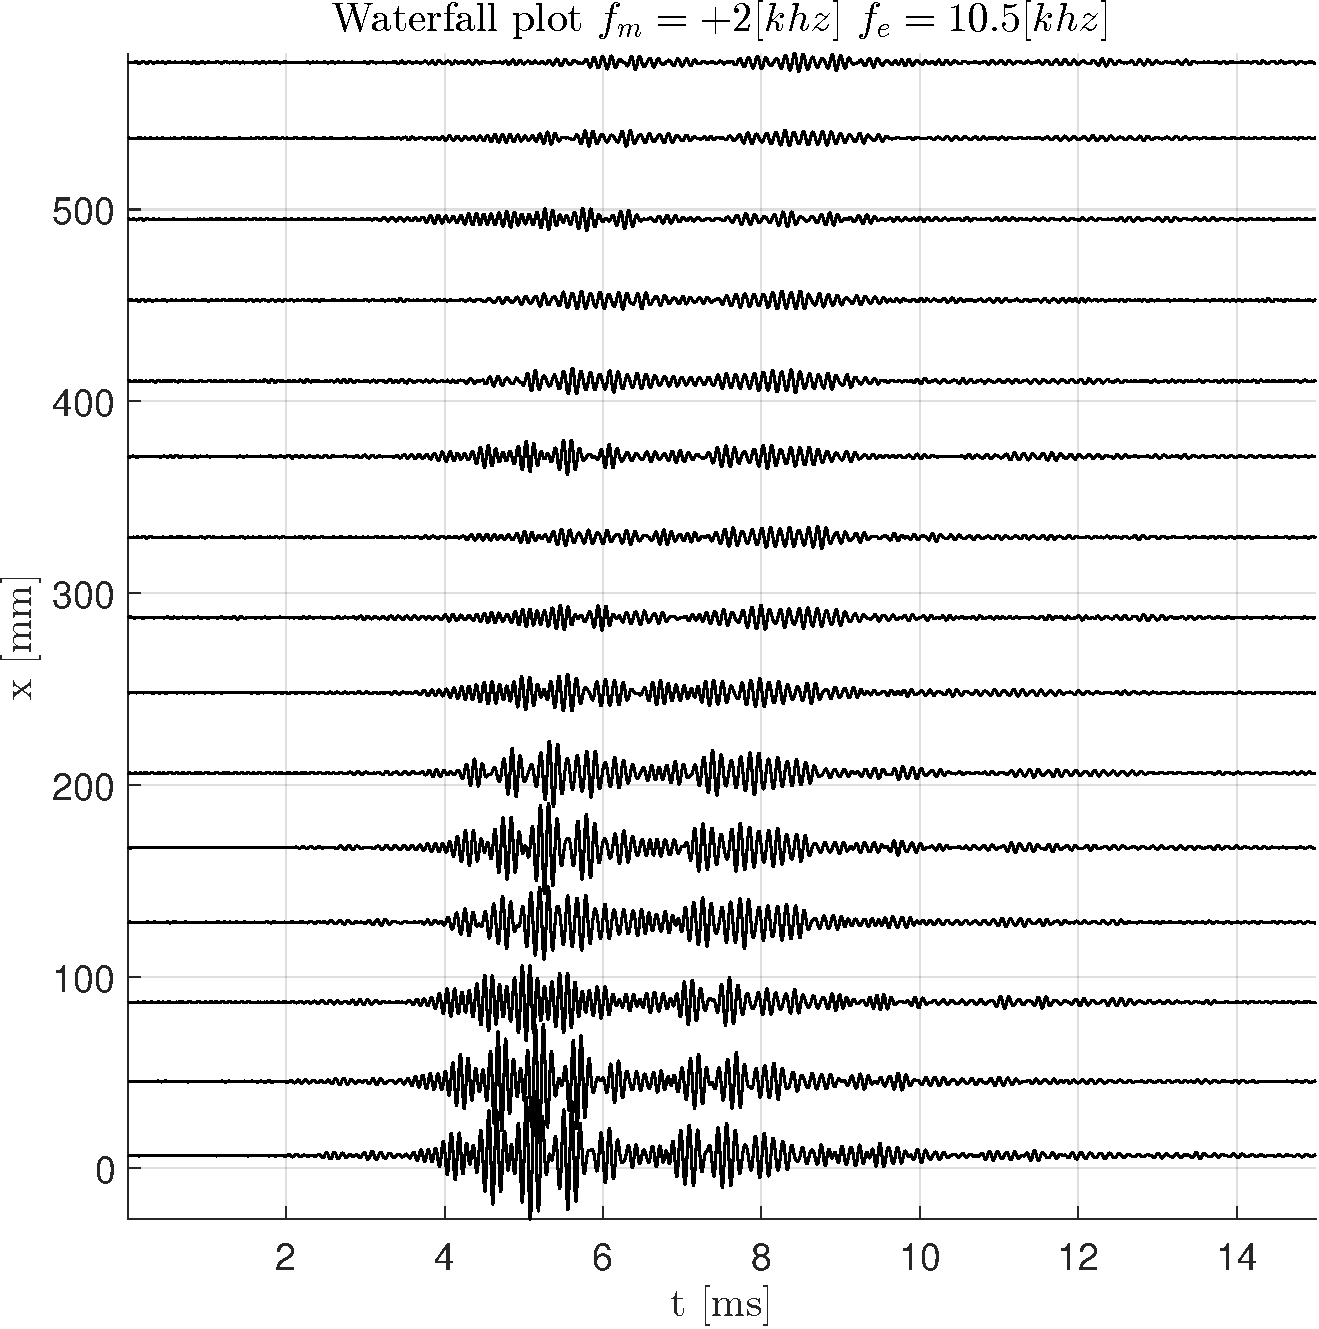
\includegraphics[width=0.45\textwidth]{img/MATLAB/EXP_Scan_time_narrow10p5kHz_2000plus.unv.pdf}
    \hspace{1cm}
    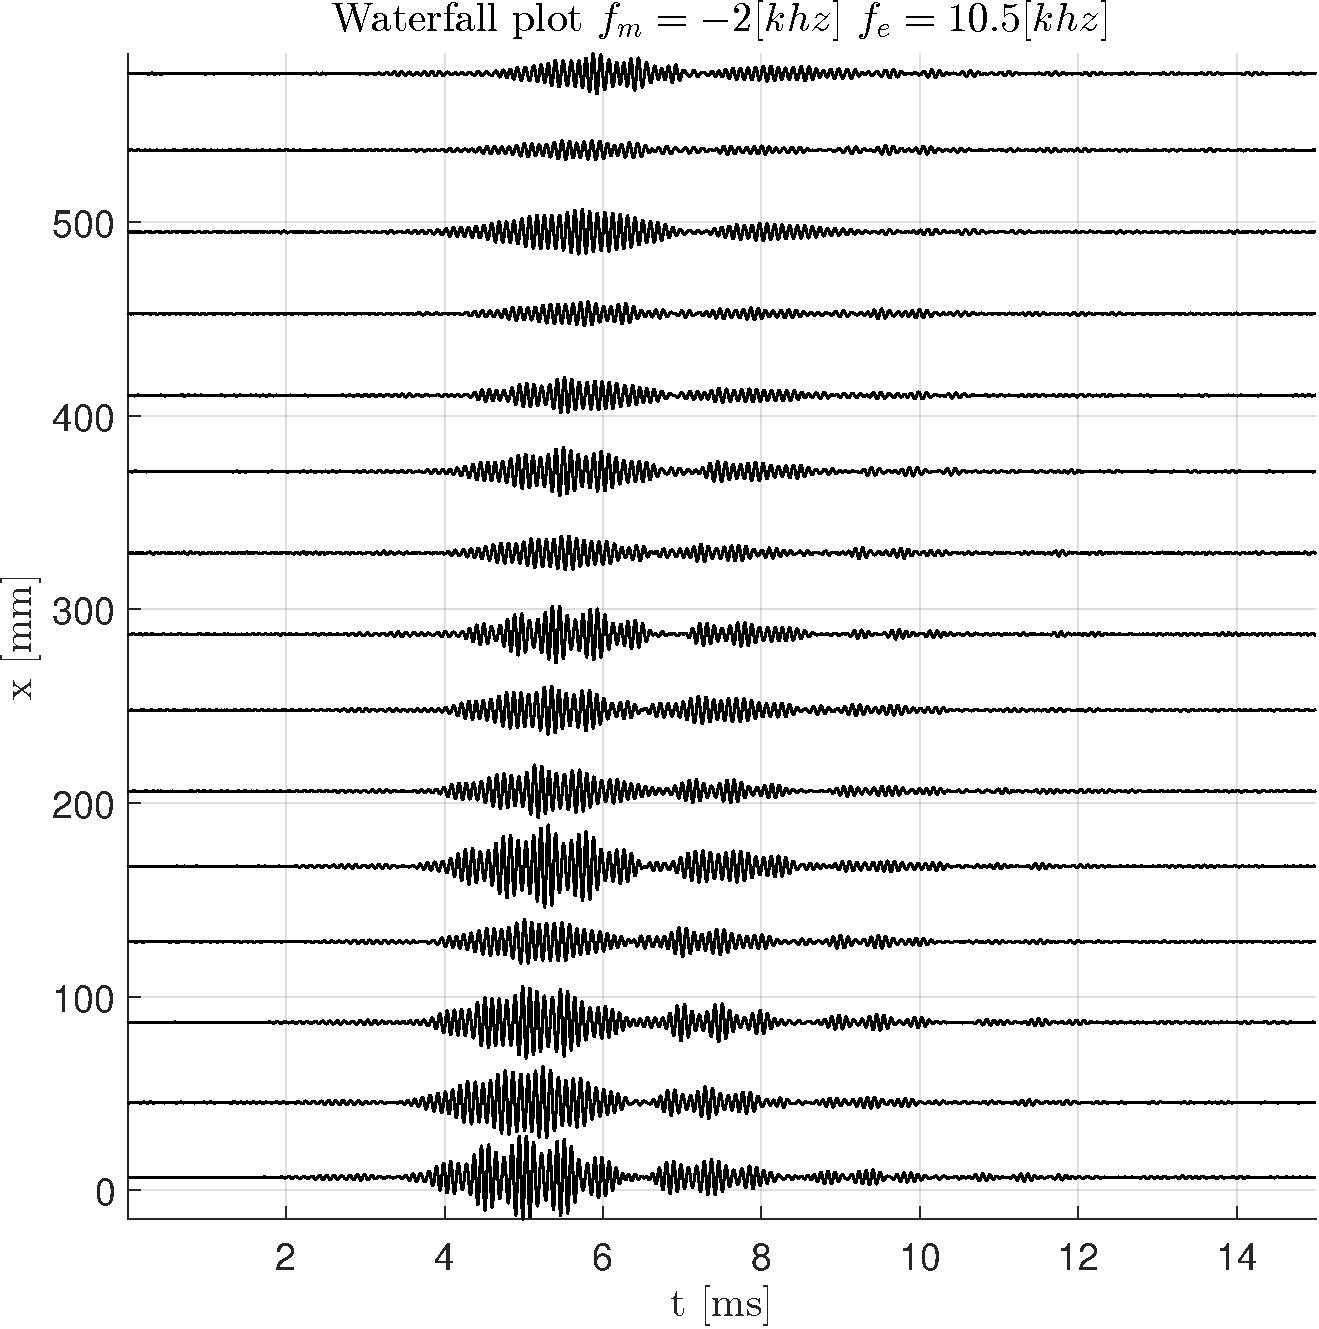
\includegraphics[width=0.45\textwidth]{img/MATLAB/EXP_Scan_time_narrow10p5kHz_2000minus.unv.pdf}
    \caption{Waterfall plot of the beam displacement for the case excitation at $f_e = 10.5 kHz$ and modulation at $f_m = +2 kHz$ (left) and $f_m = -2 kHz$ (right).}
    \label{fig:nonreciprocal_behavior_10p5kHz}
\end{figure}

The waterfall plots show a clear difference in the attenuation of the wave in the two cases.
Referring to Figure \ref{fig:nonreciprocal_behavior_2kHz}, we expected to obtain a stronger attenuation for the case of negative modulation frequency, and instead a weaker attenuation for the case of positive modulation frequency.
Figure \ref{fig:nonreciprocal_behavior_10p5kHz} confirms this expectation, showing a full band-pass behavior in one case and a full band-stop behavior in the other case.

The spectra of the beam displacement at the end of the beam are shown in Figure \ref{fig:nonreciprocal_behavior_10p5kHz_spectra}.

\begin{figure}[H]
    \centering
    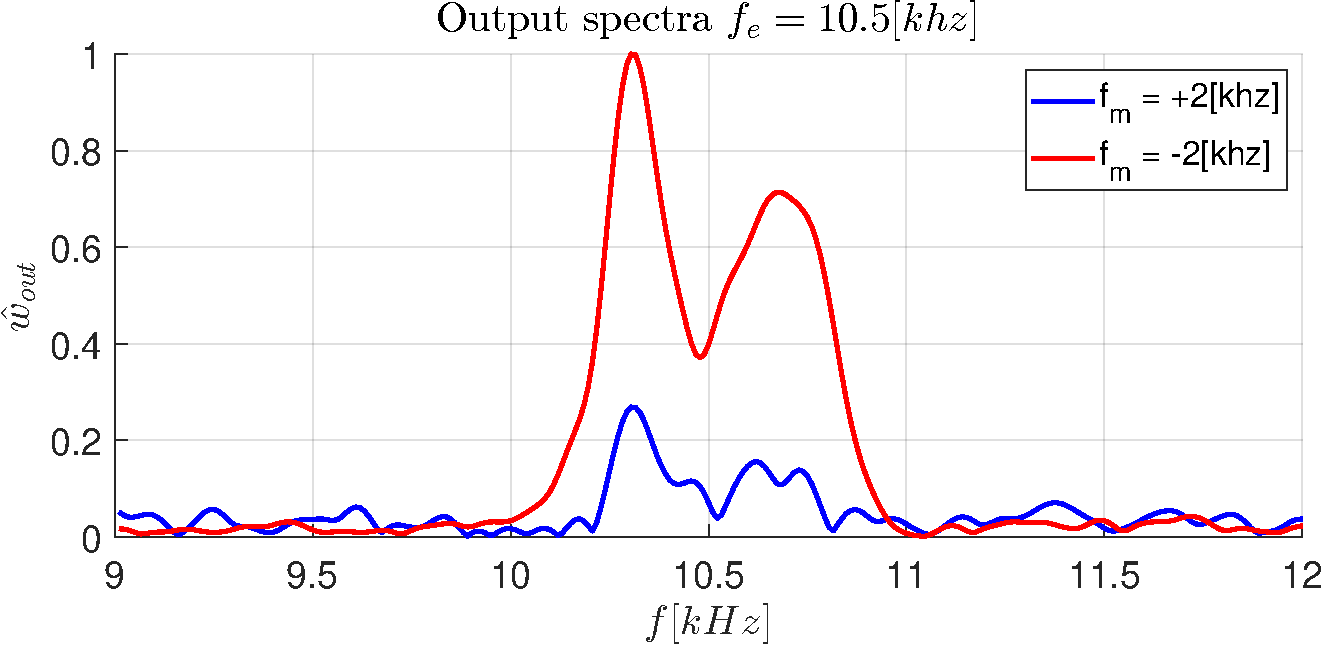
\includegraphics[width=0.7\textwidth]{img/MATLAB/Spectra_narrow10p5kHz_2000.pdf}
    \caption{Spectra of the beam displacement at the end of the beam for the case of excitation at $f_e = 10.5 kHz$ and modulation at $f_m = \pm 2 kHz$.}
    \label{fig:nonreciprocal_behavior_10p5kHz_spectra}
\end{figure}

Also the spectra analysis confirms the expected behavior.



\section{Conclusions}
\label{sec:conclusions}

This study has successfully proven the possibility of achieving nonreciprocal behavior in time-space modulated beam structures.
The experimental results confirm the feasibility of direct piezoelectric modulation as a means to achieve nonreciprocal wave propagation.
The implementation of traveling elasticity profiles through properly timed negative-capacitance shunts allows for the control of wave propagation directionality.
The result is a diode-like behavior in the wave transmission, where the wave is allowed to propagate in one direction while being blocked in the opposite direction if a directional band-gap is present.

Furthermore, the proposed setup can be adopted in microelectromechanical systems (MEMS) to achieve advanced wave control mechanisms.
The ability to precisely modulate wave propagation using compact and tunable piezoelectric elements paves the way for a variety of engineering applications such as information transmission and sensing.

Future work may focus on refining the modulation strategies to achieve even greater control over wave propagation and exploring the scalability of this approach to other types of metamaterials and metastructures.
The insights gained from this research provide a foundation for further exploration into novel applications of time-space modulated structures in wave engineering.




\vspace*{\fill}
\nocite{*}
\bibliographystyle{plain}
\bibliography{bibliography}

\end{document}
